
\documentclass[12pt]{gatech-thesis}
\usepackage{cite}
\usepackage{amsmath,amssymb,latexsym,epsfig,subfigure}
\usepackage{verbatim}
\usepackage{listings}
\usepackage{tabu}
\usepackage{booktabs}
\usepackage{floatrow}
\floatsetup[table]{capposition=top}
\usepackage{xspace}
\usepackage{hhline}
\newcommand*{\eg}{e.g.\@\xspace}
\newcommand*{\ie}{i.e.\@\xspace}

\makeatletter
\newcommand*{\etc}{%
  \@ifnextchar{.}%
              {etc}%
              {etc.\@\xspace}%
}
\makeatother

%\thesisproposaltrue

\title{Analyzing Software using Unintentional Electromagnetic Emanations from Computing Devices} %%  \protect\\ instead of \\

\author{Robert L. Callan}
\department{School of Electrical and Computer Engineering}

%\principaladvisor{Professor Alenka Zajic}
\committeechair{Professor Alenka Zajic}
\firstreader{Professor Milos Prvulovic, Co-Advisor}[School of Computer Science, College of Computing]
\secondreader{Professor Moinuddin K. Qureshi}
\thirdreader{Professor Tushar Krishna} 
\fourthreader{Professor Alessandro Orso}[School of Computer Science, College of Computing]
\fifthreader{Professor Raheem Beyah}

%\setcounter{secnumdepth}{2}
\degree{Doctor of Philosophy}

%% Set \listmajortrue below, then uncomment and set this for
%% interdisciplinary PhD programs so that the title page says
%% ``[degree] in [major]'' and puts the department at the bottom of
%% the page, rather than saying ``[degree] in the [department]''

%% \major{Algorithms, Combinatorics, and Optimization} 

\copyrightyear{2017}
\copyrighttrue
\submitdate{December 2016} % Must be the month and year of graduation,
                         % not thesis approval! As of 2010, this means
                         % this text must be May, August, or December
                         % followed by the year.

%% The date the last committee member signs the thesis form. Printed
%% on the approval page.
\approveddate{November 8, 2016}

\bibfiles{thesis}

%% The following are the defaults
%%    \titlepagetrue
%%    \signaturepagetrue
%%    \copyrightfalse
%%    \figurespagetrue
%%    \tablespagetrue
%%    \contentspagetrue
%%    \dedicationheadingfalse
%%    \bibpagetrue
%%    \thesisproposalfalse
%%    \strictmarginstrue
%%    \dissertationfalse
%%    \listmajorfalse
%%    \multivolumefalse

\begin{document}
\bibliographystyle{gatech-thesis}
%%


\newcommand{\SAVATfull}[0] {Signal Available to Attacker\xspace}
\newcommand{\SAVAT}[0] {SAVAT\xspace}
\newcommand{\zop}{\textsc{ZOP}\xspace}

\begin{preliminary}
\begin{dedication}
  I dedicate this thesis to my parents Bob and Kathee Callan, to my brother Casey Callan, and to my girlfriend Christine Godwin.

  I would have quit long ago without their patience, love, and support. 
\end{dedication}


\begin{acknowledgements}
  I would like to thank my advisors, Dr. Alenka Zajic and Dr. Milos Prvulovic, for the opportunity to work on this interesting topic. Their time, ideas, feedback, and support made the completion of this thesis possible.

  I also would like to thank my thesis committee:  Dr. Alessandro Orso, Dr. Moinuddin K. Qureshi, Dr. Tushar Krishna, and Dr. Raheem Beyah. Their time and inputs were essential in improving this thesis.
\end{acknowledgements}
\contents


%\begin{preface}
%\end{preface}


% print table of contents, figures and tables here.
% if you need a "List of Symbols or Abbreviations" look into
% gatech-thesis-gloss.sty.




\begin{summary}

This thesis develops methods to identify, quantify, and use information leaked in Electromagnetic (EM) emanations from a broad range of computing devices in a general (\ie not application specific) way by synthesizing techniques from the fields of electromagnetics, computer architecture, and software engineering. Computers emit EM radiation (emanations) as a side effect of the voltage and current variations required to perform computation. Electromagnetic Compatibility (EMC) research does systematically characterize and analyze such EM emanations, but EMC testing only identifies and quantifies EM emanations for the purpose of designing and testing computing systems to ensure emissions don't interfere with communications signals or other devices. Therefore EMC ignores any information embedded in the emissions and treats all emanations as unwanted ``noise'' whose level must be minimized. Until recently, the study of information embedded (\ie leaked) in this EM noise was limited to the leakage of sensitive information for security applications such as cryptoanalysis. Cryptography researchers have developed techniques that analyze EM emanations to extract secret cryptographic keys from computing devices as the devices perform encryption operations. These techniques generally are ad-hoc and application specific, as the goal is to demonstrate and fix weaknesses in existing cryptographic hardware and software implementations. These weaknesses can often be found without thoroughly understanding their electromagnetic and computer architectural causes. 

Aside from cryptoanalysis, EM emanations provide information about a system's operation that may be useful in other applications. A number of emerging applications make use of EM emanations to extract new types of information from computing devices. For example, EM emanations can be used to determine or verify the execution path through a program for program profiling, debugging, and malware detection. These new applications require a more general approach that can be rapidly and automatically applied to numerous and diverse types of programs and computing devices. This approach requires automatic and systematic identification, quantification, and analysis of information embedded in EM emanations. Toward this goal, our research has developed (1) a methodology for quantifying the side channel signal created by single instruction differences in a computer programs, (2) a method for identifying existing signals within computing devices which are unintentionally amplitude modulated by program activity, (3) a method for profiling computer programs via EM emanations with zero hardware and software overhead, and (4) a method for detecting the presence of unknown code during executions of a known computer program using EM emanations alone at a distance of 3 meters. 

\end{summary}
\end{preliminary}

%%
% What is purpose of introduction or other sections?
\chapter{Introduction}
\section{Motivation}
Previous research has thoroughly studied how program activity on computing devices can leak sensitive information. At first such research was conducted only in secret~\cite{Khun03}, and then publicly to address the leakage of information from CRT displays~\cite{Eck85}, and next resurged again in the field of side channel cryptoanalysis~\cite{Kocher99}. Recent research has demonstrated that EM emanations leak information about a very wide range of system activities and that this leaked information might be useful for many new applications such as profiling, malware detection, and debugging. These new applications differ from the typical cryptoanalysis side channel attack scenario in several ways. First, system designers employ countermeasures against side channel attacks that weaken the signal, increase noise, and weaken the link between the emanations and leaked information. In these new applications, however, the monitored system is not hostile and so no countermeasures are present, making the extraction of useful information from EM emanations less difficult. Second, the structure of information needed for the new applications is more complex and varies from application to application and from problem instance to problem instance. Side channel attacks typically attempt to extract a secret key (a set of a few hundred bits which are used repeatedly to encrypt or decrypt data), whereas the new applications attempt to extract more complex information, such as the execution path through a program. Finally, the reward for demonstrating a successful side channel attack against a single device is relatively high. In comparison, the reward for demonstrating these new applications of EM emanations on a single device and single program is lower. 

These differences show that the new applications require a different approach. While an application specific and effort intensive approach makes sense for side channel attacks, the new applications can take advantage of stronger (unguarded) signals but also must systematically characterize hardware and software differences between problem instances and must automatically carry out many of the steps which could be done manually during side channel attacks. In order to be viable, analyses for these new applications must also be automatically applicable across a wider variety of devices, software types, and types of information to be extracted. These analyses therefore require systematic and automated identification, quantification, and usage of EM emanations. 

%Specifically, we need to automatically 1) identify the leakage caused by specific circuits and instructions using SAVAT, 2) find which signals are modulated by useful information using FASE, and 3) automatically determine the structure of a program to be profiled and make the connection between this structure and the observed EM emanations as is done during Zero Overhead Profiling and during malware detection.

\section{SAVAT: A Practical Methodology for Measuring the Side-Channel Signal Available to the Attacker for~Instruction~Level~Events}

Previous studies of the information embedded in EM emanations have focused almost exclusively on how emanations can be used to compromise a device's security. Specifically, EM emanations have been used in a variety of side channel attacks to circumvent traditional security protections and access controls in many different types of computing devices. Unlike traditional attacks that exploit vulnerabilities in what the system does, side channel attacks access information by observing how the system does it. Computation generates many types of electronic and microarchitectural activities. Side channel attacks identify some physical or microarchitectural signal (\ie the side channel signal) that leaks desired information about system activity or the data being processed, and then analyze that signal as the system operates. Much work has been done to prevent particular side channel attacks, either by severing the tie between sensitive information and the side channel signal, or by trying to make the signal more difficult to measure. As attacks are found system designers modify and improve systems to reduce and remove very specific types of information leakage (most commonly the leakage of cryptographic keys). This makes such work very application specific and focused on a perpetual cycle of developing attacks and defenses for increasingly specific vulnerabilities. With each iteration of attack and countermeasure, the information leakage becomes weaker or harder to extract, making the attacks and countermeasures increasingly sophisticated and application specific. Furthermore, the countermeasures are often applied \textit{after} the attack methods have been discovered. Other approaches to defending against side channel attacks include adding metal shielding and introducing large amounts of random electronic noise to the system. These approaches are typically applied globally to the whole system, making them expensive and power hungry. The technique we propose, SAVAT, differs from all these approaches because it is both proactive (i.e. can be used before an attack occurs) and allows fixes which can be targeted locally at the leaking circuitry or code. 
 %Because of countermeasures, existing methods used for side channel attacks are relatively effort intensive, requiring significant work to get the attack to work on a single device and single version of a single program or implementation. 

Information leakage can be quantified at many levels of granularity, ranging from differences in emanations across phases of a program's execution down to information leakage caused by specific hardware components such as transistors. However, in order to identify specific leaking circuits or parts of a computer program, a level of granularity is required that simultaneously exposes the contributions of both hardware and software, \ie the instruction level. SAVAT quantifies information leakage at the instruction level and develops benchmarks which can be used to quantify information leakage from specific instructions and system activities such as arithmetic operations or memory accesses. We also present measurements demonstrating the usefulness, reliability, and repeatability of SAVAT, as well as a theoretical model showing that SAVAT does measure values that can be used to quantify how single instruction differences affect side channel signals in the time domain. 

\section{FASE: Finding Amplitude-modulated Side-channel Emanations}

Information leakage in computing devices can be caused by many different system components and occurs across the EM spectrum, and leakage signals are obscured by noise created by other system components and signals from the external environment such as radio broadcasts, wireless communications, and power equipment. Many of the most useful leakage signals are generated by system components that generate strong periodic signals (carriers) which are modulated by the information of interest. In order to effectively use (or minimize) the information embedded in these modulated EM emanations, it is necessary to determine system activities that modulate these carriers, determine the frequency range and strength of the leaked signals, and determine the modulation mechanisms causing the leakage. FASE presents a method for finding existing computer system signals that are amplitude modulated by a specific type of system activity. We will also present measurements showing the types of signals FASE can find, and present an algorithm for automatically finding leakage signals using FASE.

\section{ZOP: Zero-Overhead Profiling via EM Emanations}

Applications that analyze software via EM emanations must be automatically applied to arbitrary computer programs running on computing devices. Zero-Overhead Profiling (ZOP) is one such application. ZOP uses EM emanations to generate path profiles for computer programs without using any instrumentation during profiling. A program profiler dynamically analyzes a program to collect statistics about the program's behavior. Path profiling counts the number of times a specific static path occurs in the execution of a program. This type of profiling is used to identify the most commonly executed paths (or regions) of a program. This information is very useful for code optimization and performance analysis. Path profiling is usually implemented by either adding instrumentation to the profiled program that counts the executions of each desired path as the program runs, or by using dedicated hardware features to record this information. 

Using instrumentation can provide perfectly accurate profiling information (i.e. the exact number of times a particular static path occurred), but the instrumentation code adds some runtime and space overhead to the original program which is undesirable. Runtime overhead can change the control flow of a program if that program interactions with the real world (e.g. has realtime deadlines, is part of a cyberphysical system, etc.). This makes profiling such systems challenging, especially when the goal is to observe the system ``in the field'' without disturbing it. ZOP, in contrast, uses zero instrumentation and requires no hardware features, making it especially desirable for these scenarios, and desirable in any scenario where overhead is unacceptable or undesirable. The tradeoff for zero overhead is that ZOP is not perfectly accurate, though ZOP's accuracy is high enough for most profiling usage cases. We show how ZOP uses a training phase to develop a model of how EM emanations can be related to program behavior, specifically how we can extract example EM waveforms that correspond to short sections of program execution by observing EM emanations while the program is running a set of training inputs, and how based on EM emanations alone we can systematically uses these training waveforms to predict a program profile over a separate set of program executions. We demonstrate ZOP on three small control-flow oriented benchmarks, showing that ZOP can profile control flow with high accuracy. We also characterize how training input coverage affects ZOP's performance. 

\section{Detection of Unknown Code on Internet of Things Devices at a Distance}

Detection of previously unseen malware is a challenging problem, particularly on Internet of Things devices. Such devices are vulnerable to malware because their functionality requires them to be connected to the internet. They are difficult to secure because they have limited hardware and software resources, diverse software and hardware environments are used in their development, and because updating such devices is difficult. IoT devices can be attractive for malicious purposes such as Distributed Denial of Service attacks because they are produced and deployed in large volumes. These properties make monitoring and verifying control via EM emanations attractive, particularly since there is an airgap between the monitor and the monitored device, making it impossible for an attacker to circumvent the protections even if all device's software is compromised. 

ZOP can be used to detect unseen malware by predicting the control flow through the program, while simultaneously keeping track of the confidence of its predictions over the course of the program. When the monitored system only runs known code, ZOP's prediction confidence will be high through the entire run of a program since the observed waveform behavior should match the training waveform behavior well. If, however, unknown code (e.g. malware) runs on the device, new program activity (and therefore new waveform behavior) will be observed, and ZOP's confidence in its predictions will drop. Therefore, we can predict the presence of malware by observing the confidence of ZOP's predictions.

This application will also require the monitoring device to be separated from the to-be-monitored devices so that numerous devices can be monitored by a single monitor, and so that the monitoring is unobtrusive. This work also presents some more detailed characterization of the EM emanations used by ZOP, specifically presenting a method for quantifying ZOP signal quality, and showing how antennas and distance affect the signals used.

\section{Research Contributions}
The research contributions of this thesis are
\begin{itemize}
\item SAVAT, a practical methodology for measuring the side-channel signal available to the attacker for instruction-level events~\cite{CALLAN2014}
\item A comparison of SAVAT values across laptops, desktops, and an FPGA-based processor~\cite{Callan2015EMC} 
\item Measurements demonstrating SAVAT's utility, reliability, repeatability, and validity~\cite{Callan2015}
\item FASE, a method for finding amplitude-modulated side channel EM emanations~\cite{FASE_2015}
\item An algorithm for automating FASE~\cite{wang2016}
\item ZOP, a method for path profiling computer programs with zero hardware and software overhead~\cite{zop}
\item A demonstration of detecting unknown code on an IoT device at a distance of 3 meters
\end{itemize}

\section{Thesis Outline}
The remainder of this thesis is organized as follows. Chapter~\ref{sec:literature_survey} describes previous and current related research and explains how this work relates to that research. Chapter~\ref{sec:savat} describes the SAVAT methodology for quantifying an individual instruction's contribution to side channel signals, demonstrates the usage of SAVAT on laptops, desktops and an FPGA-based processor, and shows SAVAT's reliability, repeatability, and theoretical validity. Chapter~\ref{sec:fase} describes FASE, a method for finding amplitude-modulated side channel EM emanations and develops an algorithm for automating FASE.
Chapter~\ref{sec:zop} describes ZOP, a method for path profiling computer programs with zero hardware and software overhead. Chapter~\ref{sec:malware_detect} presents more detailed characterization of the EM emanations used by ZOP and how they can be used to detect unknown code, specifically presenting a method for quantifying signal quality, and showing how antennas and distance affect the signals used. Finally, Chapter~\ref{conclusions} summarizes the thesis contributions and presents possible future directions for related research.


\chapter{Background}
\label{sec:literature_survey}
This chapter reviews previous research into the uses of unintentional EM emanations. Previous studies of unintentional EM emanations mostly focused on security, specifically side channel attacks. We also review electromagnetic compatibility testing and previous work to identify and quantify side channel signals, as well as previous work on the emerging uses of EM emanations outside of side channel attacks. Finally we review traditional approaches to program profiling.

\section{Side Channel Attacks}

Traditional security vulnerabilities take advantage of security flaws in an algorithm or its implementation. In contrast, side channel attacks circumvent traditional security protections and access controls by taking advantage of the observable ``side effects'' of computation processes. Computations have side effects that are observable through many channels. A few such channels are power consumption~\cite{Bayrak11,Goubin99,Kocher99,Messerges99}, sound~\cite{Backes10,Rao02b,ShamirWeb}, behavior under faults~\cite{Biham97,giraud_aes03}, performance of shared caches~\cite{Bangerter11,tsunoo_ita02,Wang07}, and branch predictors~\cite{Aciicmez07}.

Computations in electronic circuits draw currents which often depend on the data being processed, and these currents generate EM emanations. These currents can depend directly on the data being processed. For example a data value of 0 may draw less current than a data value of 1, but additional data dependent emanations may be more subtle. For example, accessing array element A[X] may cause a cache hit or cache miss depending on the data value X. A cache miss draws much more current than a cache hit, and so the EM emanations caused by these currents will be different as well. As another example, consider an encryption algorithm (such as RSA) that performs a different computation depending whether a secret key bit is 0 or 1. Since different computations generate different EM emanations, we may be able to infer the secret key bit's value if we can determine which computation occurred by observing EM emanations. Therefore the \textit{differences in instruction execution} caused by different data values may generate much stronger EM side-channel emanations than the data values themselves, particularly for high performance processors with highly optimized microarchitecture. 

The quintessential side channel attack is Differential Power Analysis (DPA)~\cite{Kocher99}. DPA is a side channel attack carried out on a device's power signal to extract the secret key used for encryption in algorithms such as the Advanced Encryption Standard. DPA treats the computing system as a black box where the observed emanations are a direct yet unknown function of the secret key bits. Therefore DPA is suited for directly relating observed emanations to a relatively small number of secret bits where the relationship between the emanations and secret bits is unknown and the leakage signal may be very weak due to countermeasures. 

A number of methods have been developed that exploit side-channel signals to extract sensitive information. Simple microcontrollers such as those used in smartcards have been shown to be vulnerable to numerous side channel attacks such as differential power analysis. Previous work has also quantified side-channel signals generated by processor instructions using knowledge of the processor's pipeline to determine exactly when a test instruction is executing to extract a signature for each instruction type, though this technique requires sampling the side-channel signals at many times the processor clock frequency~\cite{Goldack, eisenbarth2010, Quisquater2002}. 

In general, side channel attacks are carried out by 1) identifying some physical or microarchitectural ``signal'' that ``leaks'' desired information about system activity or the data it processes, and then 2) monitoring and analyzing that signal as the system operates. Much work has been done to prevent particular side channel attacks, either by severing the tie between sensitive information and the side channel signal, or by trying to make the signal more difficult to measure. However, such work mostly focuses on preventing a particular side channel attack in a very specific piece of code, such as a cryptographic kernel. Quantifying side channel exposure in general has not been well studied, and when it has been studied, the measurements use granularity which is either very coarse (e.g. program phases) or very fine-grain granularity (e.g. at the transistor level). 

% (rewrite this sentence).

\section{The EM Side Channel}

This work primarily investigates the electromagnetic emanations side channel. It is easy to verify that electronic circuits within computing devices generate electromagetic radiation that somehow depends on the activity on the device~\cite{Rao02,Durak1999}. The security risks due to the EM side channel have been reported in the open literature as early as 1966~\cite{Highland86} but descriptions of specific risks, eavesdropping techniques, and mitigation strategies followed slowly. EM emanations from CRT monitors create particularly strong signals, exposing the monitor's contents to attackers hundreds of meters away ~\cite{Eck85,Khun03}.

Differential Power Analysis (DPA)~\cite{Kocher99} was a major breakthrough in side channel analysis, and opened up many attack possibilities, including new attacks on cryptographic implementations. Researchers have adapted DPA to use EM emanations to compromise the security of many types of devices~\cite{Rao02} from keyboards~\cite{Pasini10} to smartcards~\cite{kasper2009,Olivier01} to desktop computers~\cite{genkin_2014}.

\section{Electromagnetic Compatibility (EMC)}

EM interference/compatibility (EMI/EMC~\cite{HenryW.Ott2009},~\cite{Paul06}) techniques offer a systematic approach to the search for emanations sources. Although there has been significant research and applied work to reduce EM emanations for EMC, that work is mostly focused on interference a system can cause in other devices and in radio communications. EMC techniques therefore find \textit{all} emanations sources, not just those that leak information. This means that EMC cannot be directly used to identify and quantify leakage sources because typical computing devices have thousands of EM emanation sources but only a few that leak information. Most solutions to EMC problems also alleviate EM side-channel leakage, but some EM side-channel countermeasures hinder EMC compliance. For example, adding metal shielding for EMC compliance also attenuates EM side-channel signals, but transmission of jamming signals masks EM side-channel signals while negatively affecting EMC. Because EM emanations (such as clocks and switching regulator power signals) are subject to EMI regulations~\cite{erickson_2001}, spread-spectrum clocking and other techniques are used to spread the resulting EM emanations over a range of frequencies~\cite{hardin_1994} to minimize the maximum emanation strength. Recent findings have shown that EM signals from computer systems can still be detected in side-channel attacks~\cite{Seto13} at significant distances even for EMC compliant systems.
%cite IntelCorporation1999

\section{Identifying and Quantifying Side Channel Information Leakage Signals}

\label{sec:id_quant_em}
Strategies for quantifying potential side channel exposure {\em at the microarchitectural and architectural levels} are still not well understood. The Side-Channel Vulnerability Factor (SVF)~\cite{Demme_SVF_ISCA12,Demme_SVF_TopPicks12} measures how a side channel signal correlates with high-level execution patterns (e.g. program phase transitions). While this metric allows overall assessment of the ``leakiness'' of a particular system and application over a given side channel, it provides limited insight to (1) computer architects about which architectural and microarchitectural features are the strongest leakers, and to (2) software developers about how to reduce the side channel leakiness of their code. Other work~\cite{Goldack, eisenbarth2010, Quisquater2002} has quantified side-channel signals generated by processor instructions using knowledge of the processor's pipeline to determine exactly when a test instruction is executing to extract a signature for each instruction type. These technique can not be applied to complex devices such as smartphones and laptops because the techniques (1) require detailed knowledge of the device's microarchitecture, (2) only work for devices with very simple architecture and microarchitecture, (3) don't address external memory interfaces and (4) require sampling the side-channel signals at many times the processor clock frequency. 

Before EM information leakage can be mitigated or exploited, EM emanations that have some dependence on the information of interest must first be identified. Many EM attacks identify a range of frequencies where EM emanations depend on a secret key bit, then demodulate the signal at those frequencies or filter out unusable frequencies~\cite{gebotys2005,meynard2011,sugawara2009}. Many side channel attack descriptions only briefly or implicitly address the underlying mechanisms that cause information leakage because finding information carrying signals and determining their causes are separate processes, and because secret information can be extracted without knowing what causes the information leakage. However, both the root cause of information leakage and the leakage mechanism must be determined to mitigate leakage. This knowledge is also extremely useful for developing new applications of EM emanations.

Numerous EM emanations side channel leakage evaluation methods and countermeasure techniques have been proposed~\cite{Olivier01,seto09,Suzuki10,Sekiguchi12,Khun13,Samyde01,Tanaka08,hayashi_2013,Seto13,Hayashi13a} including the use of asynchronous circuits~\cite{Taylor03}, low-cost shielding (e.g. metal foil)~\cite{Plos08}, and transmission of jamming signals~\cite{Poucheret10}. %cite tlva method
These leakage evaluation methods and countermeasures rely on ad-hoc approaches that find a rudimentary relationship between EM emanation signals and secret key bits by observing program activities in the time or frequency domains over many key values. Since these approaches are based on the leakage of secret keys, they are specific to cryptography applications and do not identify the circuits or computer architecture mechanisms causing the leakage.

% this could use more citations
%direct emanations~\cite{Rao02a}
\section{Spectral Properties of Amplitude Modulated Non-Ideal Carriers}
\label{am_spectra}
Unintentional AM signals in computer systems have some properties not typically found in traditional uses of AM signals (i.e. telecommunications). To understand why FASE is needed and how it uses generated modulation patterns to identify AM-modulated signals, a review of the general properties of AM modulation and the irregularities of ``accidental'' side-channel transmission is needed. 

\begin{figure}[htb]
  \centering
    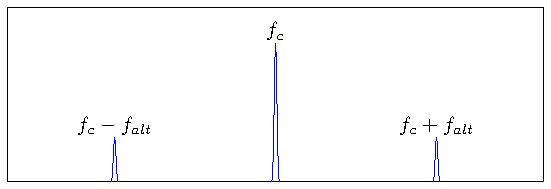
\includegraphics[scale=.95]{../fase/Data/am_details_a.pdf}
  \caption{Sinusoidal carrier modulated by a sinusoidal signal.}
  \label{am_details_a}
\end{figure}

Figure~\ref{am_details_a} shows the spectrum of an ideal carrier signal (at frequency $f_c$) that is modulated by an ideal sinusoidal signal at frequency $f_{alt}$. In addition to the carrier signal, this spectrum has strong ``side-band'' signals offset by $f_{alt}$, i.e. at frequencies $f_c - f_{alt}$ and $f_c + f_{alt}$. This would be the spectral pattern to look for when a periodic signal has a perfectly stable frequency and is modulated by a pattern of activity with a fixed period of $T_{alt} = 1/f_{alt}$ with no variation in timing but these ideal conditions are rarely present in unintentional signals.

\begin{figure}[thb]
  \centering
    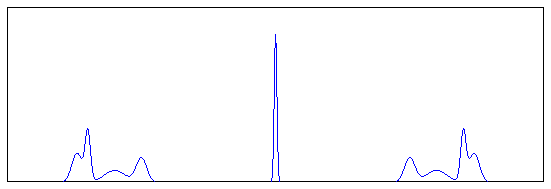
\includegraphics[scale=.95]{../fase/Data/am_details_b.pdf}
  \caption{Sinusoidal carrier modulated by an arbitrary signal.}
  \label{am_details_b}
\end{figure}

Figure~\ref{am_details_b} shows the spectrum of an ideal sinusoidal carrier modulated by an realistic baseband signal. The two side-band signals now correspond to the spectrum of the modulating activity. The tallest spike in each side-band signal corresponds to the dominant periodic behavior of that activity and the smaller ``bumps'' in each side-band signal indicate other common periods of repetitive activity. 

\begin{figure}[h]
  \centering
    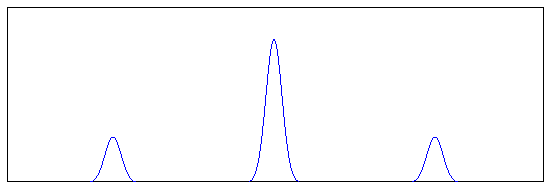
\includegraphics[scale=.95]{../fase/Data/am_details_c.pdf}
  \caption{Non-ideal carrier modulated by a sinusoidal signal.}
  \label{am_details_c}
\end{figure}

Figure~\ref{am_details_c} shows a non-ideal carrier modulated by an ideal signal. The spectrum for the carrier is now spread around its nominal value and this spreading is also present in the two side-band signals. Even though the $f_{alt}$ sinusoid is perfectly stable, the side-bands at $f_c - f_{alt}$ and $f_c + f_{alt}$ will ``inherit'' the instability of $f_c$. Many periodic signals are spread out in this manner in computer systems. For example, spread-spectrum clocking results in deliberate spreading of the clock signal's frequency. Additionally, many periodic activities (e.g. voltage regulator switching) do not require precise timing, so they often use less stable (cheaper/simpler) oscillators. Combining a non-ideal carrier (Figure~\ref{am_details_c}) with a non-ideal modulating activity (Figure~\ref{am_details_b}) produces the spectrum in Figure~\ref{am_details_d}. These non-idealities are typical for program-generated repetitive behavior: for a given task, the time each repetition of the task takes is not always the same, but there are often several commonly-occurring execution times among the repetitions. For example, in multi-processor or SMT systems the repetitions of a loop may take longer or shorter depending on timing variations due to resource contention with other running threads. 

\begin{figure}[thb]
  \centering
    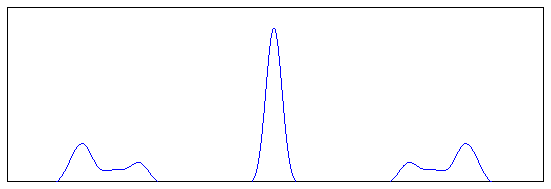
\includegraphics[scale=.95]{../fase/Data/am_details_d.pdf}
  \caption{Non-ideal carrier modulated by an arbitrary signal.}
  \label{am_details_d}
\end{figure}

\section{EM Side Channel Information Leakage on Complex Devices}

Research interest in EM side channel attacks on processors increased with the adoption of smartcards (\eg EMV ``chip'' credit/debit cards). Smartcards have processors operating at speeds less than 30 MHz and usually execute a single cryptographic program. EM emanations resulting from this program activity can leak information about embedded cryptographic keys~\cite{Rao02, Olivier01}. These processors have extremely simple architecture and micro-architecture such as 8-bit and 16-bit data widths, no branch prediction, no data or instruction caches, and small on-chip RAM with deterministic single cycle memory access times.

Despite the ubiquity of cryptographic applications in servers, desktops, laptops, and smartphones there are relatively few published applications of EM emanations targeting complex computing devices such as multi-core, multi-threaded processors with out-of-order execution and external memory interfaces. Attacking such devices is difficult because performance optimizations make emanations more difficult to analyze and because many side-channel attacks require capturing signals at a sampling rate much faster than device's clock rate, which is impractical for GHz clocks~\cite{genkin_2014}. Despite these difficulties, it has been shown that information can be transmitted several meters by EM emanations~\cite{Durak1999}, even in the presence of significant countermeasures (metal shielding, walls, etc.)~\cite{Zajic14}, and cryptographic keys can be extracted from modern computers using EM side-channel analysis~\cite{genkin_2014}. From an EMC perspective, these more powerful systems require more sophisticated components (such as processor and external DRAM memory), larger currents, longer wires, and higher switching frequencies, which all create stronger EM emanations. Therefore the information leakage in these systems may be significant yet difficult to measure and analyze.
%cite something

\section{Emerging EM Emanations Applications Beyond Side Channel Attacks}

Recent work has proposed using side channel EM emanations for several new applications such as disassembling a running program based on EM emanations alone~\cite{eisenbarth2010, scandalee}, instruction profiling for security~\cite{msgna2014}, and also verifying control flow to detect the insertion of malware or other intrusions~\cite{msgna2014_verifying,becker2012,msgna2013}. These existing approaches typically focus on identifying individual instructions (which does not work on complex devices for reasons described in Section~\ref{sec:id_quant_em}) and do not address predicting control flow through entire realistic programs. 

Several other works have shown that some system behaviors in complex devices can be recognized on long timescales. For example, web pages loaded by a device can be distinguished~\cite{Crampton2013}, and malware can be detected~\cite{clark2013} by observing current fluctuations in a power outlet. These approaches treat the leakage mechanism connecting the desired information about the system to the EM emanations as a black box, similar to cryptographic side channel attacks such as DPA. Extracting complex and abstract information about program behavior is difficult with this black box approach. For example, the control flow through a program can be determined or verified by determining whether each branch encountered is taken or not taken. This in itself requires detailed analysis and knowledge of the structure of the program being analyzed, and this structure is different for every different program analyzed. Furthermore, in order to determine the path taken we also need to determine the \textit{time} at which each branch occurs which requires further knowledge of the time required to execute each basic block in the program. 

\section{Traditional Program Profiling}

Program profiling information is used for code optimization (\eg \cite{Debray:2002:PCC:512529.512542}), testing and debugging (\eg \cite{Chilimbi:2009:HES:1555001.1555020}), and software maintenance (\eg \cite{Ernst:1999:DDL:302405.302467}). Unfortunately, obtaining code profiles, and in particular path profiles, requires code instrumentation, which is invasive and comes at the cost of high runtime overhead. The path profiling algorithm proposed by Ball and Larus~\cite{Ball:1996:EPP:243846.243857}, for instance, is an efficient (acyclic) path profiling technique that forms the basis of many other path profilers. This technique was reported to impose an average runtime overhead of 50\%, with as much as a 132\% overhead in the worst case.  Other studies (\eg
\cite{Bond:2005:PPP:1048922.1048988,Vaswani:2007:PPP:1190216.1190268}) also report similarly high overhead.

A number of techniques have been proposed by researchers to reduce the overhead of profiling. Many of these approaches try to extend or modify Ball and Larus's technique. Selective path profiling techniques (\eg \cite{Vaswani:2007:PPP:1190216.1190268,Bond:2005:PPP:1048922.1048988,Apiwattanapong:2002:SPP:586094.586104, ProfilingSelectedPathsWithLoops}) aim to reduce the overhead of path profiling by selecting a given set of paths, based on the observation that only a subset of program paths are normally of interest. Targeted path profiling~\cite{Joshi:2004:TPP:977395.977660} is another related approach that tries to reduce the execution overhead by not instrumenting the regions in the code where information could be obtained using edge profiling. Pertinent path profiling~\cite{Baswana:2013:PPP:2495258.2495922} is yet another technique that addresses the high overhead problem by optimizing the data structures used for profiling. Sampling-based instrumentation approaches (\eg ~\cite{Arnold:2001:FRC:378795.378832,  Traub00ephemeralinstrumentation}) use a different approach to reduce the cost of instrumentation and infer profiling information from a sample of runtime events. Finally, partitioned path profiling~\cite{Afraz:2015:PPP:2786805.2786868} proposes the idea of parallel path profiling, which profiles a program by evenly distributing the number of probes into multiple cores.

Despite all the work done so far to reduce the runtime overhead of instrumentation based program profiling, profiling still comes at a non-negligible cost in terms of overhead. Although this overhead is tolerable in some cases, it is not always so (\eg for embedded devices with limited resources or real-time systems). Moreover, instrumentation is an intrusive technique that can change some aspect of a program's dynamic behavior of such code, especially in the case of complex, real-time, and/or multi-threaded systems. %This system has zero overhead while profiling executions. In return for zero overhead, ZOP requires a training phase and the accuracy is imperfect. This reduction in accuracy may be acceptable for many applications.

Some systems have hardware features to assist in profiling~\cite{intel_vtune, intel_pmu, arm_pmu, shye2005}, but these features cannot completely eliminate software overhead; even hardware-accelerated profiling must somehow record profiling information, which necessarily affects the programs being profiled. External hardware tracers and debuggers~\cite{lauterbach} can profile without software overhead but require significant processor hardware support to collect and transmit traces off-chip. Using EM emanations, profiling has no in-system hardware requirements, which is particularly appealing for applications where any overhead, instrumentation, or modification is unacceptable and for systems where hardware profiling support is unavailable.


\chapter{A Practical Methodology for Measuring the Side-Channel Signal Available to the Attacker for Instruction-Level Events}
\label{sec:savat}

\section{Overview}
This chapter presents a metric, the Side-Channel Signal Available to the Attacker (SAVAT,~\cite{CALLAN2014}), which does not present or imply a specific side-channel attack, but instead provides direct quantitative feedback to programmers and hardware designers about which instructions (or combination of instructions) have the greatest potential to create side-channel vulnerabilities. For this purpose, it is best to analyze information leakage due to instruction execution because analyzing emanations at the circuit level (e.g. wires, transistors, and gates) does not address the effects of system architecture and software, and because analyzing emanations at the program or program phase level~\cite{Demme_SVF_ISCA12,Demme_SVF_TopPicks12} does not provide direct feedback to pinpoint leakage sources. SAVAT overcomes the difficulties in measuring information leakage in complex systems by generating controlled EM emanations to isolate the differences between instructions one pair at a time, and then measuring and analyzing these emanations in the frequency domain.

SAVAT measures the side channel signal created by a specific single-instruction difference in program execution. In other words, \SAVAT quantifies the signal made available to a potential attacker who wishes to decide whether the program has executed instruction/event A or instruction/event B. This level of granularity is neither too fine-grained nor too coarse, and therefore is useful to both computer architects (\SAVAT tells which microarchitectural features create strong leakage signals) and to software developers (\SAVAT allows them to systematically aggregate the leakages caused by single instruction differences throughout a program).

We also measure EM side-channel energy among several common instructions from a laptop, a desktop, and an FPGA at several different frequencies. We show that the SAVAT measurements performed at different frequencies result in comparable SAVAT values, up to a frequency dependent scale factor. We also confirm several expectations. First, the SAVAT values for a given instruction pair are much smaller on the FPGA compared to personal computers, as might be expected based on differences in power and performance levels in the systems. Second, between instruction pairs we observe similar trends across all devices. By comparing results between different systems, vulnerabilities that are consistent across several processor generations and among manufacturers can be determined, allowing designers and programmers to focus on the most endemic vulnerabilities.

To summarize, this chapter presents: 
\begin{enumerate}
\item SAVAT, a new metric that quantifies the side channel signal caused by differences in code execution at the instruction level, 
\item A practical methodology for measuring \SAVAT on real machines, 
\item A derivation proving that the methodology does measure \SAVAT given a simplified yet realistic processor and emanations model, and
\item SAVAT measurements for the EM emanations side channel for a small set of instructions for laptops, desktops, and an FPGA-based processor demonstrating SAVAT's utility, reliability, and repeatability.
%\item Simulations, measurements, and analysis comparing EM emanations \SAVAT to power \SAVAT for a NIOS processor. 
\end{enumerate}


\section{The \SAVAT Metric}
\label{savat-metric}
Assume an attacker has access to a program's source code or executable and can observe EM emanations from the victim's system while this program is running. The attacker attempts to extract sensitive information by recording EM emanations from the victim system while the program is running. The attacker then uses these recorded signals to infer which instructions are executed, and then infers sensitive data from knowledge of the executed instructions. The difficulty with which the attacker can obtain the sensitive information depends on both (1) program activity: the information-dependent difference created at the instruction level, and (2) the side channel signal's dependence on these instruction-level differences. 

The SAVAT metric quantifies this second property for a system. This allows (1) programmers to change their code to avoid creating high-\SAVAT instruction-level differences that depend on secret information, and (2) computer architects and microarchitects to focus their side channel mitigation efforts on high-\SAVAT instructions. Most side channel mitigation techniques are expensive, especially if applied very broadly. For example, circuit-level techniques that mask input-dependent variations in overall activity do so by performing more activity overall: when actual inputs require little activity, additional unnecessary activity is performed to match what happens for high-activity values. This minimizes variations in power consumption, EM activity, etc. The costs of these techniques are high: large increases in chip area (for dummy-activity circuitry), execution times that always match the worst case inputs, and power consumption that always equals the peak power consumption.

To develop a targeted approach to identifying information leakage, we will create a model that assumes that information leakage through side channels occurs when the instructions executed depend on sensitive information, and that this instruction-level difference creates a side channel signal that is available to the attacker. A program with input-dependent behavior will generate data-dependent activity in the processor and possibly also in the off-chip memory and other system components. This data-dependent activity will create signals in various side channels. Data-dependent activity in the system cannot be avoided: even if the program's control flow does not depend on the value of the input, and if the circuitry of the processor is designed such that every operand value results in the exact same overall number of bit-flips in transistors and wires, there will be at least some transistors or wires whose switching activity is input-dependent. This difference in transistor/wire activity creates a difference in various physical side channel signals, such as EM emanations, power consumption, etc. Process variations, physical location of the circuit, etc. allow side channel signals to be created even if the circuitry is designed to minimize the operand-dependent variations in overall activity -- these techniques can dramatically reduce the magnitude of data-dependent signal variation but cannot completely eliminate them. But this does not mean that these and other techniques are ineffective -- they force attackers to use more expensive, bulkier, and less widely available snooping devices, to run more risk of discovery (e.g. if they get closer to collect the weak EM emanations), and/or to need more data points and collect signals longer for the same amount of extracted information.

Many attacks rely on instruction-level differences in execution caused by data-dependence on sensitive information. For example, modular exponentiation in RSA is typically implemented in a way that results in testing the bits of the secret exponents one at time, and multiplying two large numbers (e.g. 2048 bits) whenever such a bit is 1. This entire multiplication can thus be viewed as the difference in execution caused by sensitive information (a bit of the exponent). This example also shows that, although the signal leaked by a single-instruction difference can be small, a practical attack may accumulate many of these single-instruction differences -- an entire large-numbers multiplication in this example. 

As another example, suppose an attacker can isolate (in the recorded EM signal) the time offset of a single branch instruction in the program, and suppose that this branch instruction is taken or not taken depending on a sensitive data bit. The attacker observes the side channel signal for a time period immediately following the branch. The executed instructions and/or data following the branch may be different depending on whether the branch is taken, and so the recorded signal may be different when the branch is taken or not taken. Using this signal difference, an attacker may be able to determine whether the branch is taken (and therefore determine the sensitive bit) using a procedure such as DPA. If we call the voltage signal corresponding to a taken branch $s_a(t)$ and the signal for the branch not taken $s_b(t)$, then we can estimate the total side-channel energy available to the attacker to determine whether the branch was taken as
\begin{equation}
  \textrm{SAVAT}(s_a,s_b) \equiv \int_{0}^{T_s} (s_a(t) - s_b(t))^2 dt/R
\end{equation}
where the $s_a(t)$ and $s_b(t)$ voltages are measured across a resistance $R$, and $t = (0,T_s)$ is the time interval after the tested branch where $s_a(t)$ and $s_b(t)$ differ depending on whether the branch is taken. Many other data dependent dependent activities cause such differences. For example, a signal difference may be created when a cache hit or miss occurs depending on sensitive data.

We can then rephrase the problem of quantifying this type of side channel vulnerability as calculating $\textrm{SAVAT}(s_a,s_b)$ for a given victim program and inputs without directly measuring $s_a(t)$ and $s_b(t)$. With some simplifying assumptions it is possible to calculate $\textrm{SAVAT}(s_a,s_b)$ by adding up all the single instruction differences between $s_a(t)$ and $s_b(t)$. For example, if $s_a(t)$ and $s_b(t)$ are the same except that the processor executes instruction B at some time $t_e$ during $s_b(t)$, while the processor executes instruction A at $t_e$ during $s_a(t)$, then $\textrm{SAVAT}(s_a,s_b) = \textrm{SAVAT}(A,B)$. Section~\ref{sec:methodology} presents a methodology for measuring $\textrm{SAVAT}(A,B)$ reliably using inexpensive equipment, and Appendix~\ref{appendix} presents a derivation showing that this methodology does measure $\textrm{SAVAT}(A,B)$ given a set of realistic assumptions. 

SAVAT quantifies the overall signal that is made available to the attacker through the side channel as a result of a single-instruction variation: executing a different instruction because of a control-flow decision, having or not having a cache miss, etc. The SAVAT is a pairwise metric: it measures the signal made available to the attacker when we execute instruction/event A instead of executing instruction/event B (or vice versa). For example, the ADD/MUL SAVAT is the overall side channel signal available to the attacker to determine whether we have executed an ADD or a MUL instruction, the LDM/LDL2 SAVAT is the overall amount of the side channel signal that tells the attacker whether we had a L2 hit or an off-chip memory access for a load instruction, etc. We also define the single-instruction SAVAT as the maximum of the pairwise SAVATs where both events in the pair are generated using the same instruction. For example, the SAVAT for a load instruction is the maximum of pairwise SAVATs: LDM/LDM, LDM/LDL2, LDM/LDL1, etc.

How many single-instruction differences need to be accumulated to mount a successful attack depends on the SAVAT values between these instructions -- huge SAVAT values enable attacks even when sensitive data creates a seemingly small difference in execution, e.g. the attacker may need fewer such ``loud'' instructions. Single instruction differences in execution may be accumulated in two ways: (1) repetition: the same single-instruction difference may be re-created many times, and the attacker can use the overall difference that is created, and (2) combination: entire sequences of different instructions can be executed. Our measurement methodology will exploit repetition to obtain signals that can be more reliably measured, then divides the large measured signal by the number of repetitions to determine the contribution of a single instance. Combination is not directly addressed in this work -- while we believe that the sum of single-instruction differences can act as a good estimate for the combined signal, this estimate is imprecise because instructions can be reordered and their execution may overlap. A more accurate SAVAT measurement of signal differences created by executing different sequences of instructions can be performed by using those entire sequences as A/B activity in the measurement. However, this approach does not scale well to longer sequences: pairwise SAVAT measurement for $N$ individual instructions requires $O(N^2)$ measurements, pairwise measurement among all possible two-instruction sequences constructed from these $N$ instructions requires $O(N^4)$ measurements, etc. One approach to this combinatorial explosion is to cluster instruction opcodes using SAVAT as the distance metric, then explore sequences using instruction class representatives. Another approach would be to derive a good model of the interaction among instructions in a sequence, i.e. to capture effects of reordering, dependencies, etc., and then compute overall SAVAT values for instruction sequences by using the interaction model to combine measured single-instruction SAVAT values. 


\section{Methodology for Measuring SAVAT in Real Systems}
\label{sec:methodology}
This chapter describes a methodology for directly measuring SAVAT for a pair of instructions in a system. The goal is to measure the EM emanations side-channel signal (or another type of side channel signal) created by executing instruction A vs executing instruction B (i.e. $\textrm{SAVAT}(A,B)$). A naive approach measures the signals for A and B separately, then computes the area (total amplitude difference over time) between the signal curves for A and B. Unfortunately, this naive approach has a very large measurement error. First, the single-instruction signal difference is much smaller than the overall signal generated by the execution that surrounds the instruction under examination. Complex processors heavily optimize the scheduling and execution of instructions, so determining the times where the test instructions A or B are actually active would be problematic.
Computing a small difference between two large signals is subject to huge relative error because the measurement error for each signal is proportional to the signal's overall value, i.e. the difference between signals might be dominated by measurement errors in the two measurements. Second, the computed $A - B$ signal is affected by imperfect alignment of the two signals in time. Other instructions must be present around A and B to make the measurement practical (to trigger the measurement, setup the registers and memory used by instructions A and B, etc.), and so noise and other unrelated components of the received signal obfuscate the signal components created by the A and B instructions themselves. Third, this approach requires recording many samples of the two signals (to enable accurate subtraction) over a very short period of time (the duration of a single instruction). Even the most sophisticated ($>$\$200,000 cost) instruments provide only 10-20 samples per clock cycle in modern multi-GHz processors. Equipment capable of measuring the low amplitude $a(t)$ and $b(t)$ signals at greater than 10G samples/sec (as required to test a processor using a GHz clock) is prohibitively expensive or non-existent. The naive approach for measuring an A/B SAVAT which is subject to the aforementioned problems is illustrated in Figure~\ref{NaiveMeasurement}: execute a program fragment that performs instruction/event A and record the side channel signal, then execute an identical program fragment but now with instruction/event B instead of A, record the side channel signal again, then align the two signal curves in time and compute the area between the two curves.

\begin{figure}[thb]
\centering
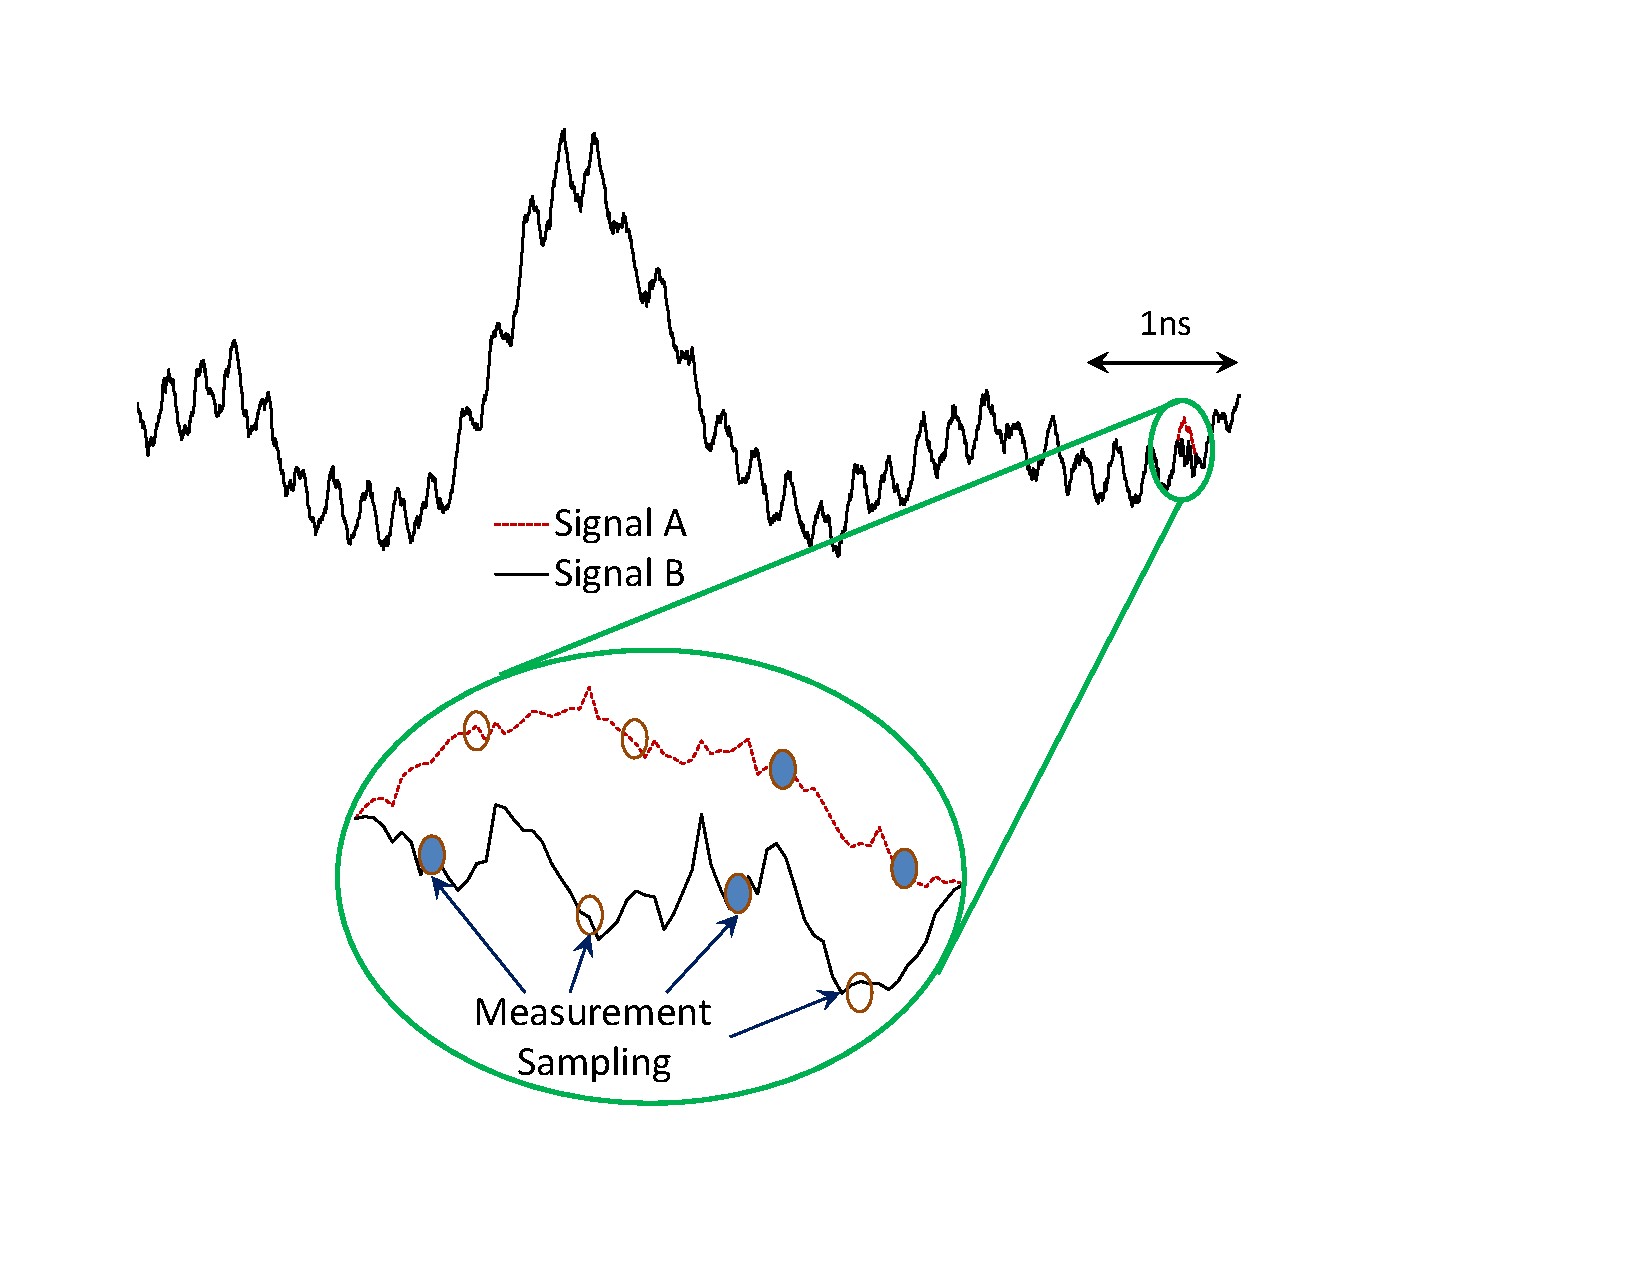
\includegraphics[trim=0.8in 1.1in 2.7in 0.8in,clip,width=5in]{../savat_final/Drawing/NaiveMeasurement.pdf}
\caption{A naive approach for measuring SAVAT.}
\label{NaiveMeasurement}
\end{figure}

To overcome these problems, our methodology employs microbenchmarks carefully constructed so that any signal due to differences between the A and B instructions is localized in frequency (Figure~\ref{PeriodicSignal}b), whereas the naive approach attempts to localize this difference in time in separate A and B signals (Figure~\ref{NaiveMeasurement}). The new A and B combined signal is constructed by having the computer system alternate between the two instructions/events (A and B) many times per second as shown in Figure~\ref{PeriodicSignal}b. This alternation generates a periodic signal at the alternation frequency that corresponds to the overall difference between the individual signals. This periodic signal can then be filtered to reject other frequencies including the noise and the uninteresting signals they carry, and the filtered signal's magnitude can then be measured. For EM emanations, power, sound, etc., this filtering and measurement can be done very precisely using a spectrum analyzer. The spectrum obtained in this way measures the difference in signal strength between A and B instructions/events over a unit time (e.g. a second), and overcomes all of the problems with the naive measurement because (1) the measured A/B difference signal accumulates over many A/B differences over this one second, effectively amplifying the signal and suppressing noise (the instrument only needs to be sensitive enough to measure the one-second total, we can still compute the single-instruction/event SAVAT by dividing the measured signal by the number of A/B instances that occur each second), (2) the difference between A and B side channel signals is directly measured, without the relative-error problem present when measuring A and B signals separately, and (3) the signal is measured at the alternation frequency, which can be adjusted in software by changing the number of A and B events per iteration of the alternation loop, so we can easily bring that frequency within the measurement range of commercially available instruments. We also have the freedom to select a frequency with relatively little noise - an important consideration for EM emanation side channels where direct collection of A and B side channel signals is subject not only to measurement error but also to noise from various radio signals. Also, while the A/B difference signal occurs at the greatly attenuated high frequencies in the naive measurement,  in this new methodology the A/B difference signal occurs at a single, known, easier-to-measure, low frequency. 

\begin{figure*}[htb]
\centering
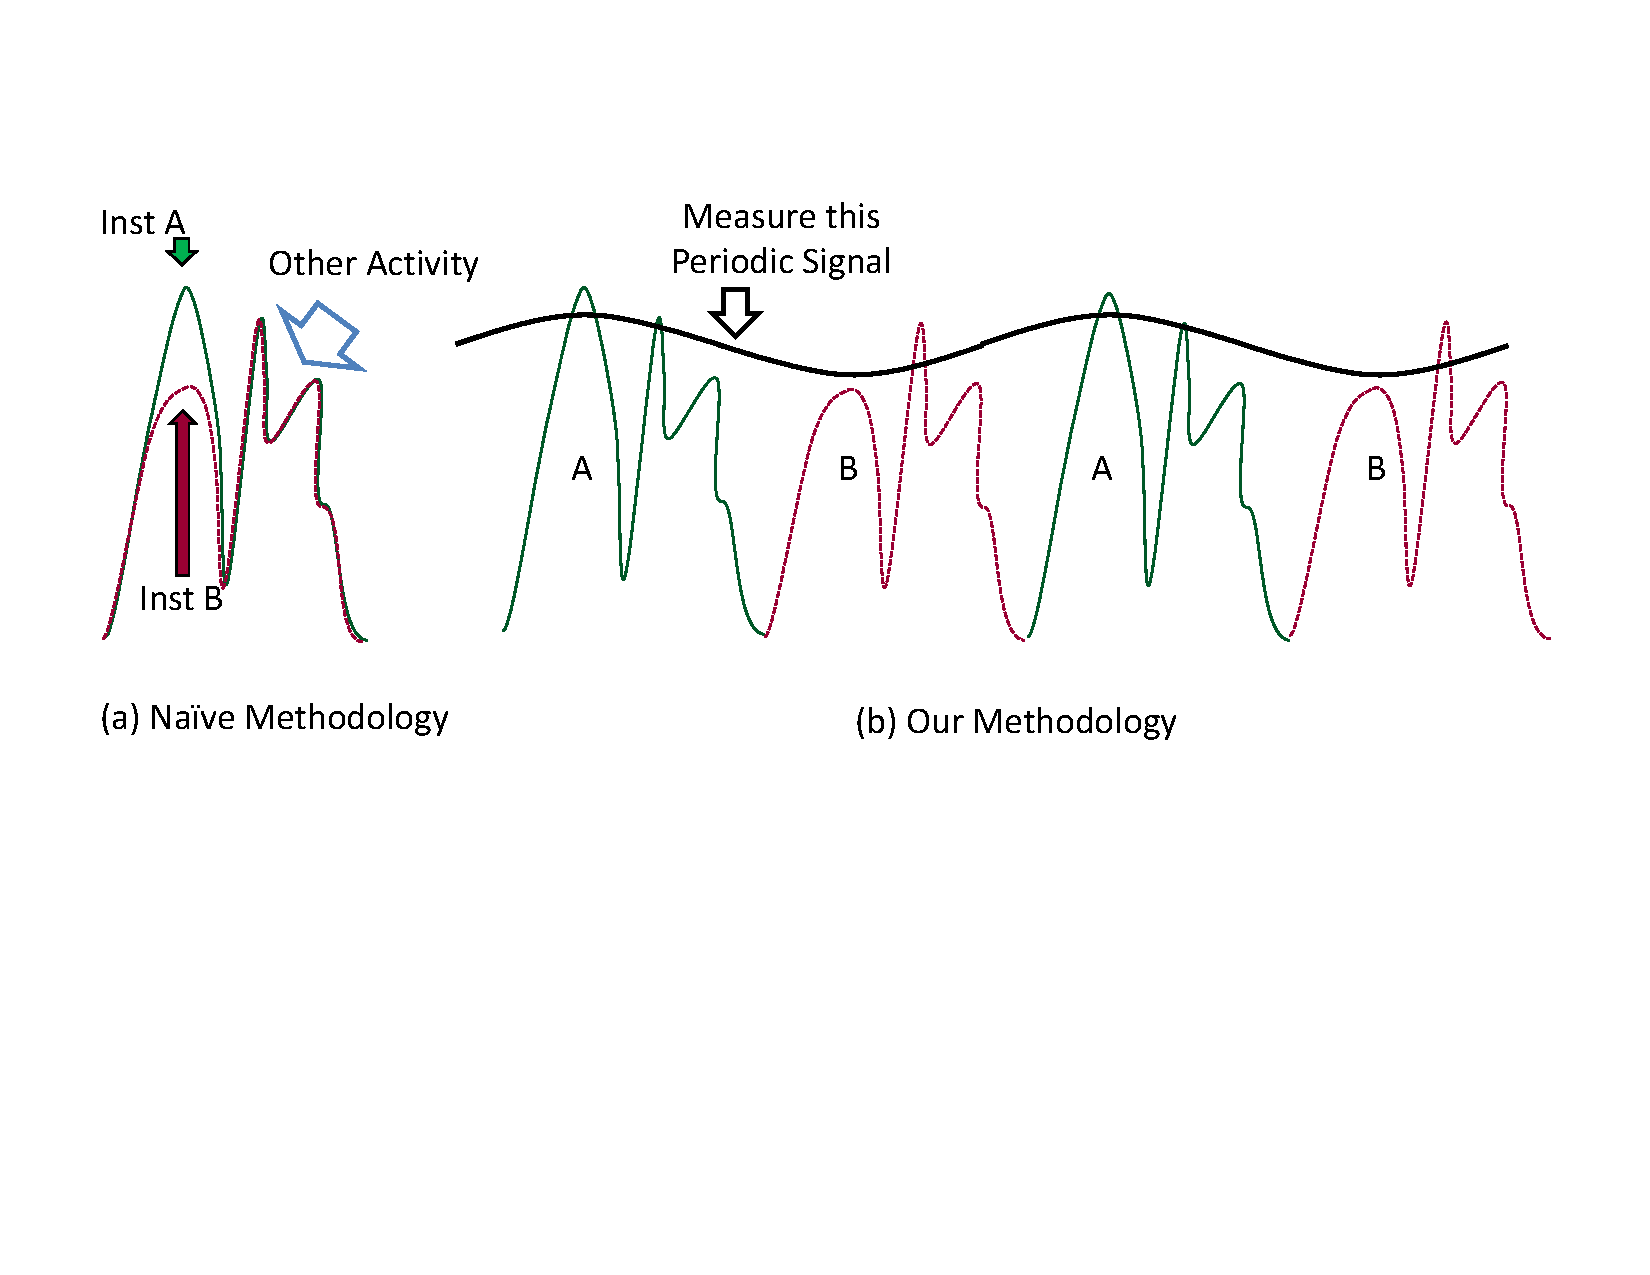
\includegraphics[trim=0.6in 3.5in 0.6in 1.3in,clip,width=6in]{../savat_final/Drawing/PeriodicSignal.pdf}
\caption{Our methodology measures the (a) signal difference by (b) alternating the signals then filtering and measuring the resulting periodic signal at the alternation frequency.}
\label{PeriodicSignal}
\end{figure*}



\begin{figure}[htb]
  \centering
\lstset{language=C++,basicstyle=\ttfamily\small,numbers=left}\lstset{escapeinside={/*@}{@*/}}
\begin{lstlisting}[frame=none,xleftmargin=30pt]
while(1){/*@\label{BegInfLoop}@*/
  // Do some instances of the A inst/event /*@\label{BegLoopA}@*/
  for(i=0;i<n_inst;i++){
    ptr1=(ptr1&~mask)|((ptr1+offset)&mask);/*@\label{UpdAddrA}@*/
    // The A-instruction, e.g. a load
    value=*ptr1;/*@\label{TestInstA}@*/
  }/*@\label{EndLoopA}@*/
  // Do some instances of the B inst/event /*@\label{BegLoopB}@*/
  for(i=0;i<n_inst;i++){
    ptr2=(ptr2&~mask)|((ptr2+offset)&mask);/*@\label{UpdAddrB}@*/
    // The B-instruction, e.g. a store
    *ptr2=value;/*@\label{TestInstB}@*/
  }/*@\label{EndLoopB}@*/
}
\end{lstlisting}
\caption{The A/B alternation pseudo-code.}\label{pseudocode}
\end{figure}

The overall structure of the code used in the measurement methodology is shown in Figure~\ref{pseudocode}. Lines \ref{BegLoopA} through \ref{EndLoopA} execute \texttt{n\_inst} instances of the A instruction/event, and then lines \ref{BegLoopB} through \ref{EndLoopB} execute the same number of instances of the B instruction. Thus lines \ref{BegLoopA} through \ref{EndLoopB} represent one A/B alternation, and this alternation is repeated (line \ref{BegInfLoop}) until the measurement of the side channel signal is complete. The value of \texttt{n\_inst} allows us to control the number of alternations per second, and we select a value that produces the desired alternation frequency for our measurements. For a given desired repetition period $T_{alt}$ corresponding to one iteration of the outer loop, $T_{alt}$ can be directly measured using counters available through processor instructions (e.g. the x86 \texttt{rdtsc} instruction) or the operating system (e.g. the Windows API \texttt{QueryPerformanceCounter()} function).  For example, increasing \texttt{n\_inst} increases the time required to execute one iteration of the outer loop ($T_{alt}$).

The benchmarks generate controllable emanations at frequency ($f_{alt} = 1/T_{alt}$) as shown in Figure~\ref{Fig:Carrier}. Intuitively we expect differences between the A and B instructions to appear at the frequency $f_{alt} = 1/T_{alt}$. More analysis is required to derive the exact relationship between the spectral power $P(f_{alt})$ (observed at $f_{alt}$ while running the A/B alternation microbenchmark) and the side channel energy available to attackers due to a single execution of instruction A instead of instruction B ($\textrm{SAVAT}(A,B)$). Appendix~\ref{appendix} describes some required assumptions and a derivation of the relationship between $P(f_{alt})$ and $\textrm{SAVAT}(A,B)$. 

\begin{figure}[htb]
  \centering
  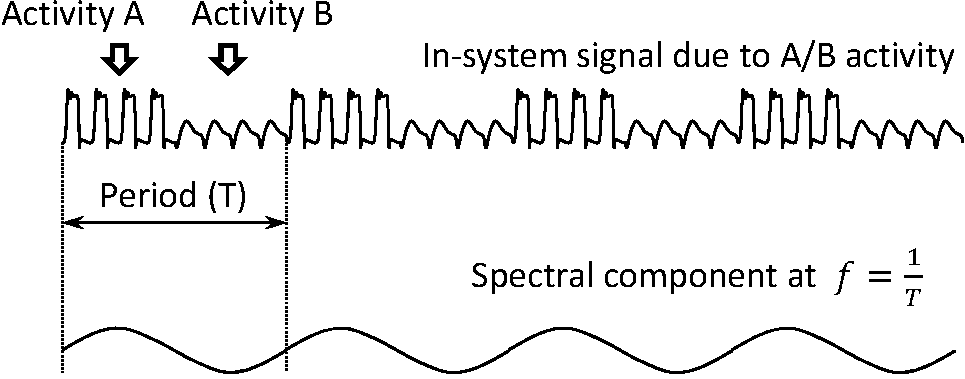
\includegraphics[scale=0.45,clip]{../TEMC_SAVAT/TEMC_314_2013_Fig1a.pdf}
  \caption{The A/B alternation pseudo-code induces emanations at a specific radio frequency by alternating half-periods of A and B activity.}
  \label{Fig:Carrier}
\end{figure}

To generate different cache behavior during load and store instructions, our code (in lines \ref{UpdAddrA} and \ref{UpdAddrB}) updates the address of the accessed memory location so the memory access repeatedly sweeps over an array of appropriate size (fits in L1 cache, does not fit in L1 but fits in L2 cache, or does not fit in L2) to create the desired cache hit/miss behavior. Note that \texttt{ptr1}, \texttt{ptr2}, and \texttt{offset} must be chosen so that the A and B instructions access separate groups of cache blocks to create the desired cache behavior (e.g. every A is a L1 cache hit and every B is a L2 cache hit). Aside from the test instructions (line \ref{TestInstA} for A and line \ref{TestInstB} for B), the executed code should be identical for all instructions/events, so this pointer-update code is present even when the A and/or B instruction is a non-memory instruction (e.g. ADD). Our actual code is written in x86 assembler to minimize the amount of non-under-test activity and prevent compiler optimizations that might make the non-under-test code differ for different under-test instructions (e.g. different instruction scheduling by the compiler, dead code elimination of memory address updates for non-memory instructions, etc.).

Measuring SAVAT using this methodology overcomes several measurement problems. First, the measured signal represents the accumulation of many repetitions of the A/B difference, so this signal can be measured with less sensitive instruments. Second, the difference between A and B side-channel SAVAT is directly measured, avoiding the relative error introduced when measuring A and B signals separately. Finally, the signal is measured at the alternation frequency, which can be adjusted in software by changing the number of A and B instructions per iteration of the alternation loop, resulting in a lower measurement frequency which is within the measurement range of commercially available instruments. We also have the freedom to select a frequency with the least interference from noise and unrelated signals. This is particularly important for the EM emanations side-channel because EM probes pick up numerous unrelated noise sources and radio signals.


\section{Experimental Setup}
\label{sec:setup}
To demonstrate the usefulness, repeatability, and validity of the SAVAT metric and methodology, we will run the SAVAT benchmarks for several instruction pairs on some computing devices and measure the resulting EM emanations. The instructions listed in Tables~\ref{insts}~and~\ref{nios_insts} were used in the A/B alternation microbenchmarks as described in Section~\ref{sec:methodology} for each pairwise instruction combination. These lists include loads and stores serviced by different levels of the cache hierarchy, simple (ADD and SUB) and more complex (MUL and DIV) integer arithmetic, and the "No instruction" case where the appropriate line in our alternation code (Line \ref{TestInstA} or \ref{TestInstB} in Figure~\ref{pseudocode}) is simply left empty. The NIOS processor has only an L1 cache so LDL2 and STL2 are not applicable. 

\begin{table}[htb]%
  \small%
  \label{insts}%
    \caption{x86 instructions for our A/B SAVAT measurements.}%
    \begin{tabular}{lll}%
    \toprule
    & \textbf{Instruction} & \textbf{Description} \\
    \midrule
    LDM  & mov eax,[esi]        & Load from main memory \\
    STM  & mov [esi],0xFFFFFFFF & Store to main memory  \\
    LDL2 & mov eax,[esi]        & Load from L2 cache    \\
    STL2 & mov [esi],0xFFFFFFFF & Store to L2 cache     \\
    LDL1 & mov eax,[esi]        & Load from L1 cache    \\
    STL1 & mov [esi],0xFFFFFFFF & Store to L1 cache     \\
    ADD  & add eax,173          & Add imm to reg  \\
    SUB  & sub eax,173          & Sub imm from reg \\
    MUL  & imul eax,173         & Integer multiplication \\
    DIV  & idiv eax             & Integer division       \\
    NOI  &                      & No instruction \\
    \bottomrule
        \end{tabular}%
\end{table}%

\begin{table}[htbp]%
  \small%
  \centering%
    \begin{tabular}{lll}%
    \toprule
    & \textbf{Instruction} & \textbf{Description} \\
    \midrule
    LDM  & ldw  r21, 0(r21) & Load from main memory \\
    STM  & stw  r21, 0(r21) & Store to main memory  \\
    LDL1 & ldw  r21, 0(r21) & Load from L1 cache    \\
    STL1 & stw  r21, 0(r21) & Store to L1 cache     \\
    ADD  & addi r22,r22,173 & Add imm to reg  \\
    SUB  & subi r22,r22,173 & Sub imm from reg \\
    MUL  & muli r22,r22,173 & Integer multiplication \\
    DIV  & div  r22,r22,r22 & Integer division       \\
    NOI  &                  & No instruction \\
    \bottomrule
    \end{tabular}%
  \caption{NIOS instructions for our DE1 FPGA A/B SAVAT measurements.}%
  \label{nios_insts}%
\end{table}%

The systems tested are listed in Table~\ref{pc_specs}, along with relevant system properties such as CPU and memory clock rates, processor microarchitecture, and cache parameters. For the laptops and desktop, the benchmarks are run as single-threaded Windows 7 32-bit user mode console applications. No other user-mode applications were active and wireless devices were disabled to minimize interference with the intentionally generated signals. Aside from this, the systems were operating normally, meaning that any EM signals resulting from system processes and other OS activity would affect the received signal. For the FPGA, the benchmarks were run on a NIOS soft processor implemented on a DE1 Cyclone II FPGA board, with no memory management or operating system. No other logic was active on the FPGA. 

\begin{table*}[tb]%
  \scriptsize%
  \centering%
    \begin{tabular}{ccccc}%
    \toprule
    \textbf{System} & \textbf{Processor} & \textbf{Memory} & \textbf{L1 Data Cache} & \textbf{L2 Cache} \\
    \midrule
    Altera DE1 FPGA      & NIOS II ``fast'', 50 MHz  & 50 MHz SDRAM  & 4 KB, 1 way & None \\
    Dell Latitude C610   & Intel Pentium IIIM, 1 GHz  & 133 MHz DDR   & 16 KB, 4 way & 512 KB, 8 way \\
    Lenovo X61           & Intel Core Duo, 1.8 GHz & 333 MHz DDR2  & 32 KB, 8 way & 4096 KB, 16 way \\
    HP Pavilion tx2000   & AMD Turion X2, 2.3 GHz & 333 MHz DDR2  & 64 KB, 2 way & 1024 KB, 16 way \\
    Dell Optiplex 7010   & Intel Core i7, 3.4 GHz & 1600 MHz DDR3 & 64 KB, 2 way & 1024 KB, 16 way \\
    \bottomrule
    \end{tabular}%
  \caption{Measured FPGA, laptop, and desktop systems.}%
  \label{pc_specs}%
\end{table*}%


EM probe type, position, and orientation affect the strength of the received emanations. A small ``sniffer'' probe placed a few millimeters above components picks up signals from only the components near the probe, but receives these signals very strongly. On the other hand, placing a probe with a larger effective area far away ($>$~2~meters) will pick up signals from all the parts of the system, but is often not sensitive enough to pick up the weakest signals. Furthermore, the strength of the emanations from the x86 systems is much stronger than the emanations from the NIOS FPGA system. Therefore, two measurement setups were used. The first setup, shown in Figure~\ref{large_setup} was used for measurements and comparisons which did not involve the FPGA system. For these measurements, the periodic EM signal at the alternation frequency was measured using a 20~cm diameter magnetic loop antenna (AOR LA400) placed at a distance of 10~cm from the tested system. This antenna does not use a tuning capacitor and is terminated with a $50\Omega$ load, so it has a flat frequency response between $10~{\rm kHz}$ and $1~{\rm MHz}$. This will be referred to as the 20~cm loop setup. A recent paper illustrates a practical EM attack on implementations of the RSA and ElGamal algorithms using similar equipment and laptops~\cite{genkin_2014}. 

\begin{figure}[htb]
\centering
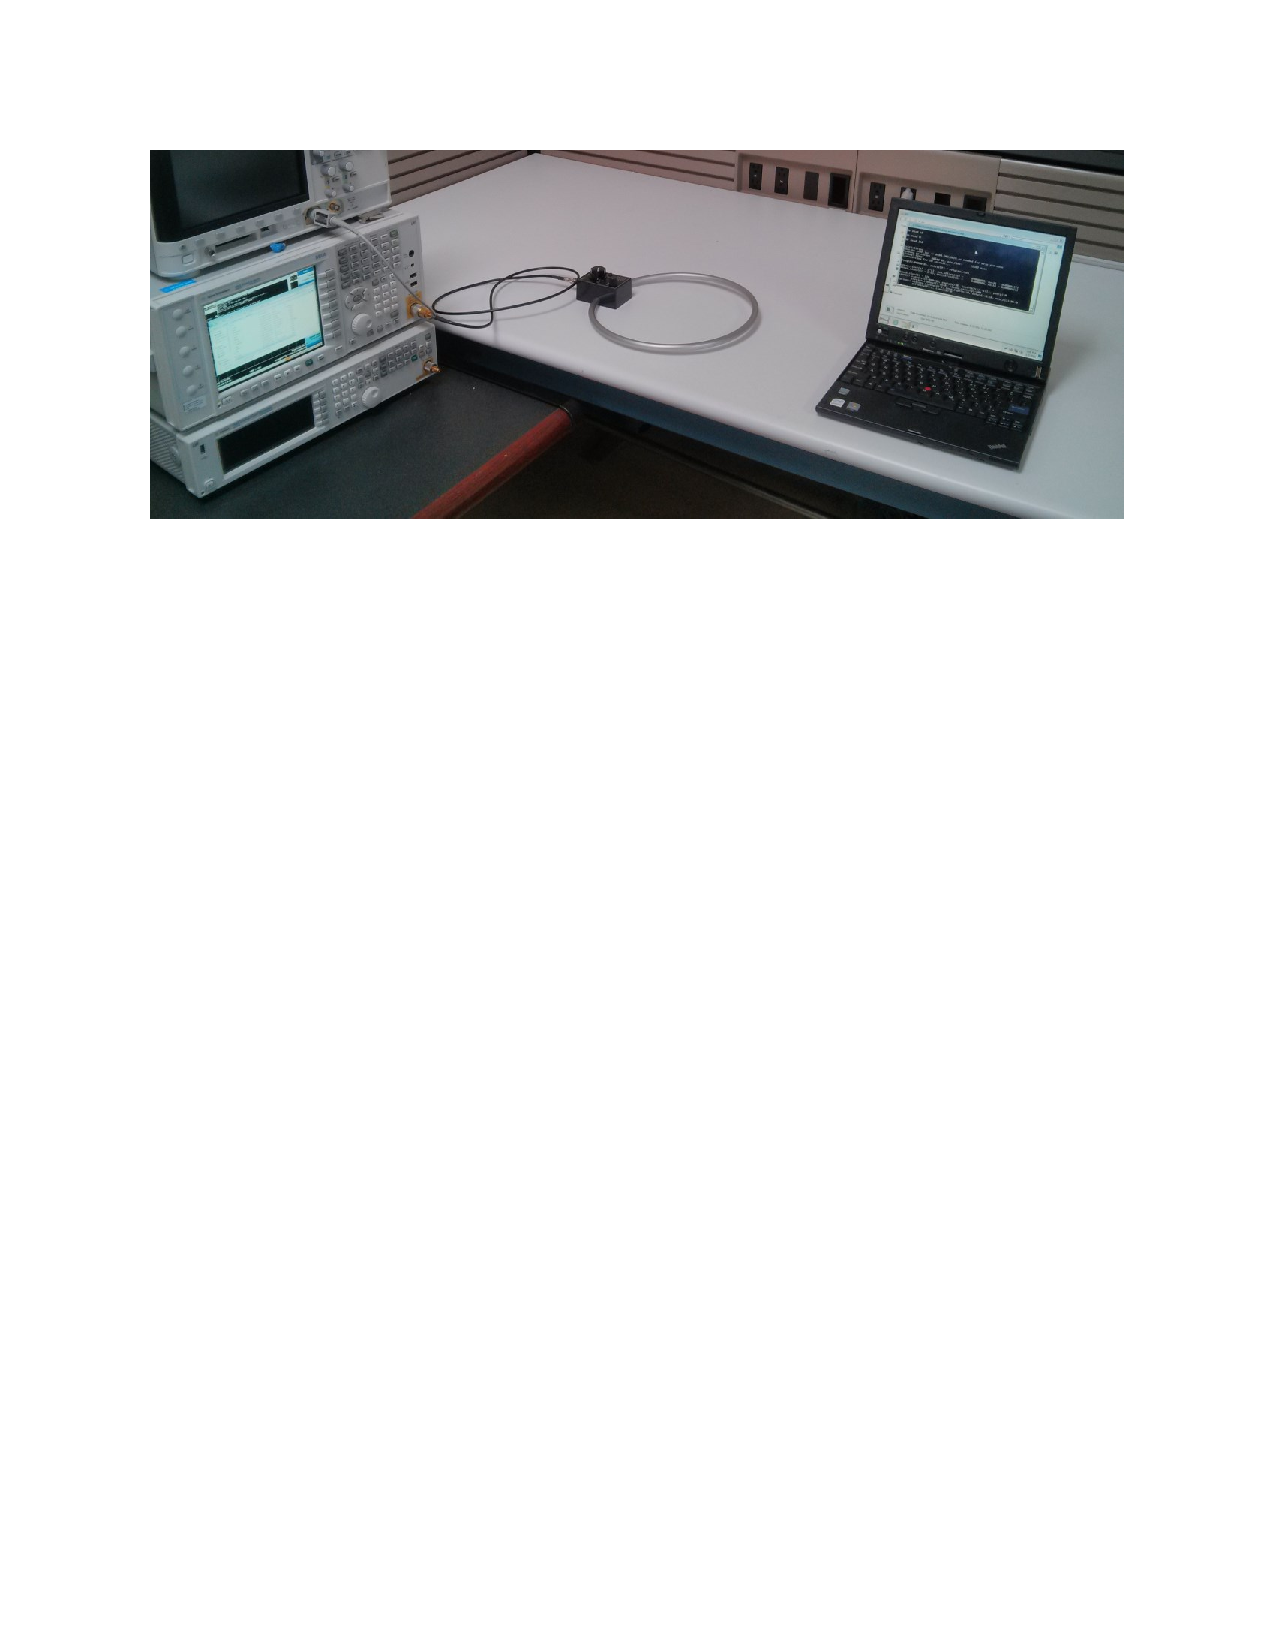
\includegraphics[bb=0.94in 7.49in 7.56in 10.01in,clip=true,width=3.4in]{../TEMC_SAVAT/setup.pdf}
\caption{Measurement setup for the 20 cm loop probe.}
\label{large_setup}
\end{figure}

To conduct a comparison between the x86-based and NIOS-based systems, the probe must pick up emanations from all the parts of the system while at the same time being close enough to pick up the weakest signals tested. A medium sized multiple turn square loop (4 cm width, 20 turns) placed 10~cm above the processor as shown in Figure~\ref{small_setup} was ideal for this purpose. This will be referred to as the 4~cm coil setup. For our measurements the loops are oriented parallel to the PCBs because the magnetic field vectors for the generated signals point in this general direction at the shown probe locations.

\begin{figure}[htb]
\centering
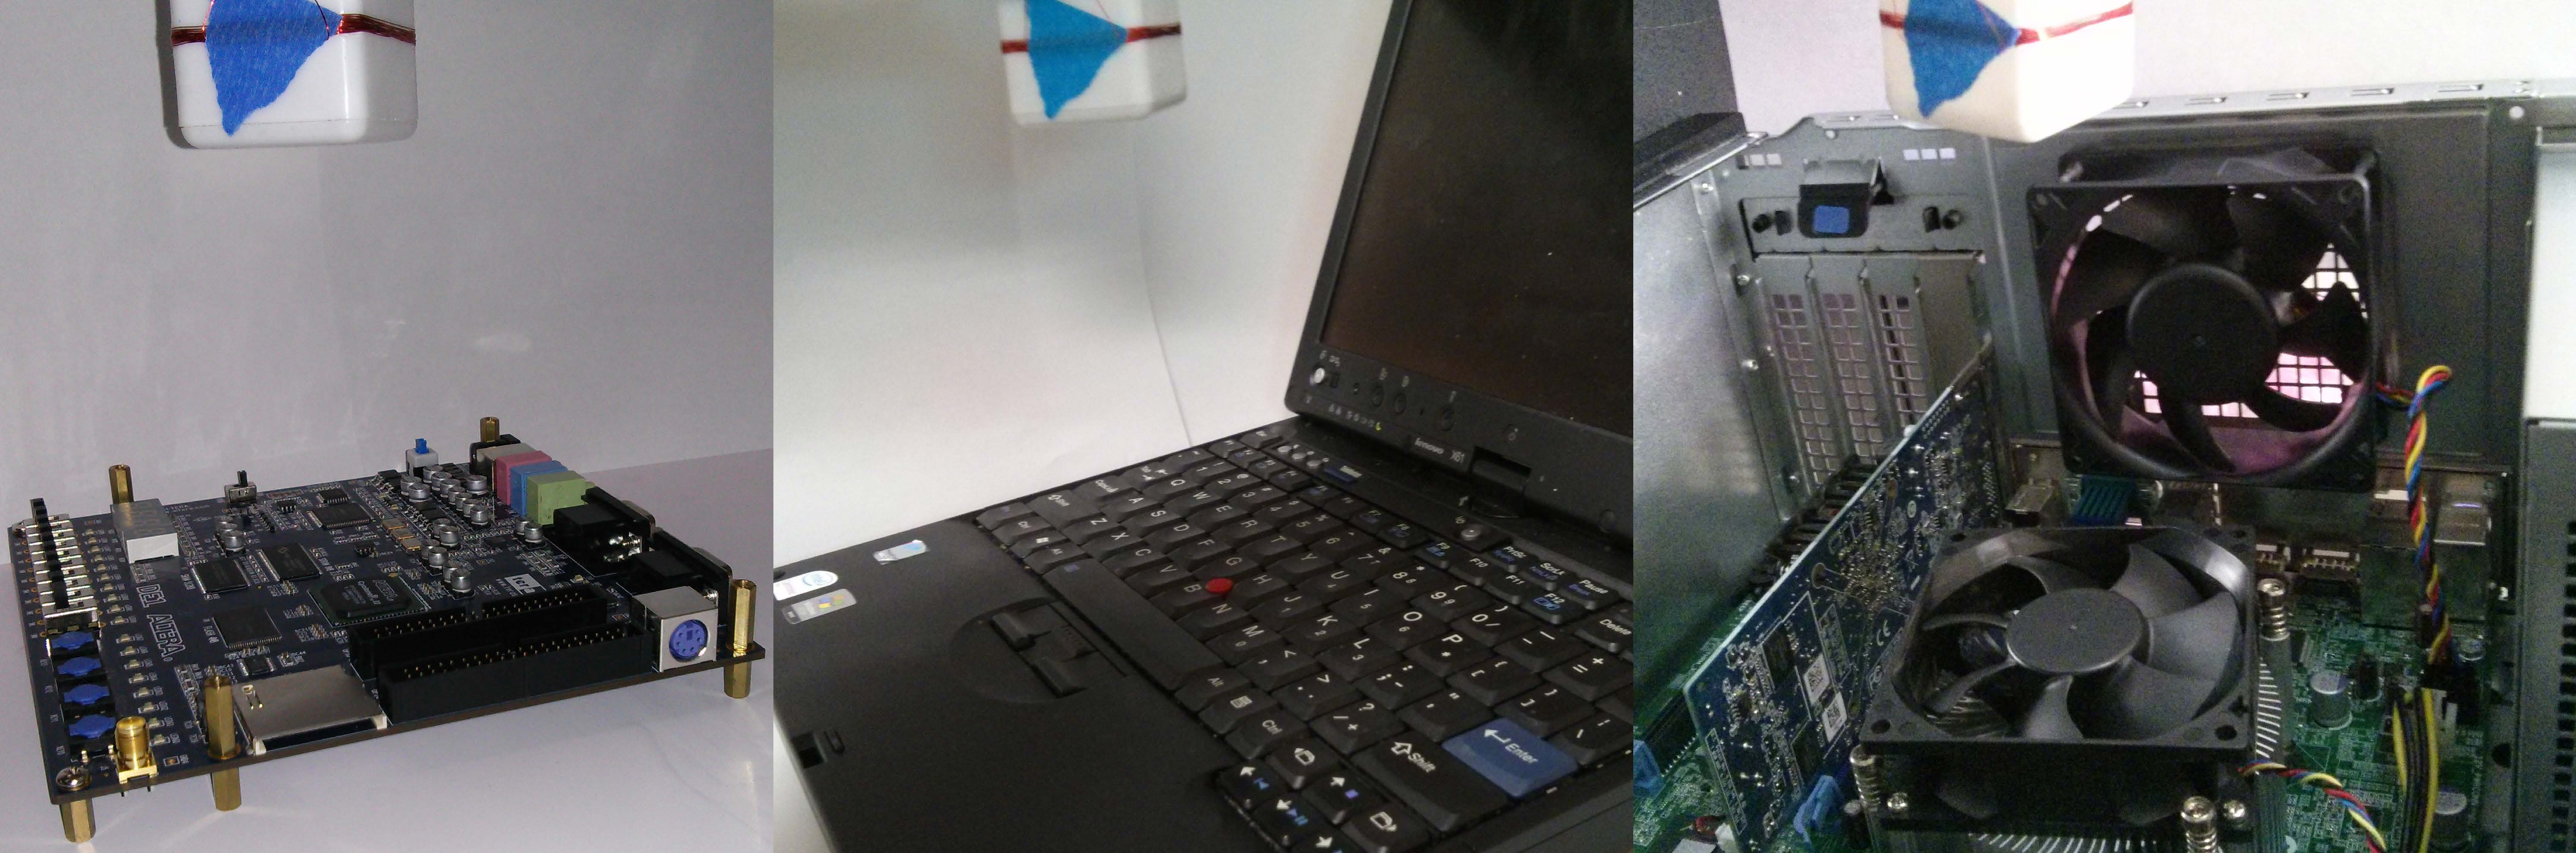
\includegraphics[width=5in]{../emc_comparison_4/setups.pdf}
\caption{FPGA (left), laptop (center), and desktop (right) measurement setups for the 4 cm coil probe.}
\label{small_setup}
\end{figure}

\begin{figure}[htb]
\centering
%\includegraphics[trim=1.4in 5.75in 1.4in 1.2in,clip,width=3.375in]{ADD-LDM-Spectrum.pdf}
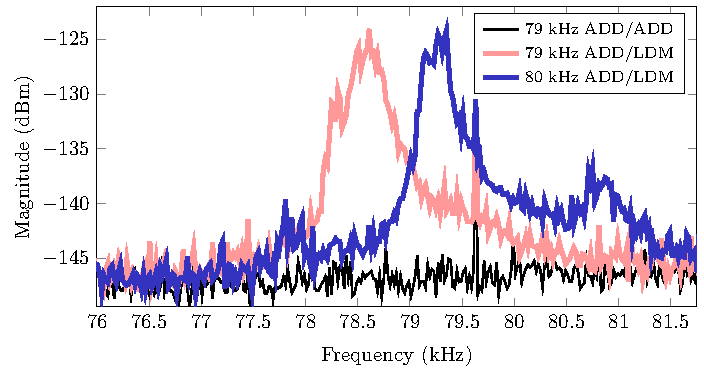
\includegraphics[width=5in]{../TEMC_SAVAT/spect_add_ldm.pdf}
\caption{Power spectrum of ADD/LDM instruction pair at $79$~kHz and $80$~kHz.}
\label{ADD-LDM-Spectrum}
\end{figure}

The power across the probes was measured using a spectrum analyzer (Agilent MXA N9020A). The spectrum around the alternation frequency was re\-cor\-ded with a resolution bandwidth of 1Hz, which results in a very low measurement noise floor because the measured signal is affected only by noise from a 1Hz-wide spectral band. Unless otherwise noted, measurements use an A/B alternation frequency of $80~{\rm kHz}$ and are collected $10~{\rm cm}$ above the device. %explain why
%power calculation?
As shown in Figure~\ref{ADD-LDM-Spectrum}, we can choose the alternation period $T_{alt}$, allowing us to avoid parts of the spectrum where other signals might be present. This spectra shows the ADD/LDM instruction pair (integer addition vs an off-chip memory load) with $79$ and $80$ kHz alternation frequencies along with an ADD/ADD measurement. 

Our measurements include all cases where A and B are the exact same instruction/event, where the resulting A/A alternation should result in no signal at the alternation frequency, such as the ADD/ADD spectrum shown in Figure~\ref{ADD-LDM-Spectrum}. We see that some signal does exist in the band around the intended alternation frequency: these signals may be caused by the instrument's sensitivity floor (which is around $-147$ dBm in Figure~\ref{ADD-LDM-Spectrum}), external radio signals, and a weak signal created by imperfect matching of A/B not-under-test activity. Therefore, these same-instruction alternation measurements give us a very good estimate of the experimental measurement error, and can help identify possible problems such as strong radio interference or mistakes in the A/B alternation code. When A and B instructions/events are not the same, we measure both the A/B alternation and the B/A alternation - these should be the same, so their difference allows us to assess the measurement error caused by placing identical instructions at different program addresses, i.e. the effect of fetch-related variations such as instruction cache alignment.

In Figure~\ref{ADD-LDM-Spectrum}, the $79$ kHz and $80$ kHz ADD/LDM spectra show broad peaks, and these peaks clearly track the alternation frequency. The shifting signals we observe are not due to other unrelated signals (such as nearby switching power supplies, CRT or LCD monitors, or other cabling) because the signal is only present when the A and B instructions differ (i.e. there is no signal for ADD/ADD), and because the observed peak follows the intended alternation frequency. The generated signals are not perfectly concentrated at the intended $f_{alt}$ because (1) $f_{alt}$ cannot be controlled perfectly in a real system and (2) the alternation period $T_{alt}$ (the time to execute one iteration of the outer loop in Figure~\ref{pseudocode}) varies slightly in complex processors and systems, resulting in the dispersion of power around the alternation frequency. For each pair of instructions A and B, we run the A/B microbenchmark and measure the power spectral density from $2.5$ kHz above to $2.5$ kHz below the alternation frequency. Then we integrate over this band to get the total power $P(f_{alt})$ generated by the difference between A and B. Finally the $\textrm{SAVAT}(A,B)$ is calculated from $P(f_{alt})$. 


\section{Experimental Results}
This section presents the following SAVAT experimental measurement results:
\begin{enumerate}
\item A case study using SAVAT to compare and contrast EM emanations from several laptops and a desktop using a 20cm loop antenna
\item A comparison of SAVAT across a laptop, desktop, and FPGA using a 4cm coil antenna
\item Measurements characterizing SAVAT's reliability and repeatability
\end{enumerate}

\subsection{SAVAT Laptop and Desktop Measurements using a 20 cm Loop Antenna}
\label{savat-20cm}

In this section, we perform a case study where we measure the EM side channel SAVAT for all possible pairings of 11 instructions selected from the x86 instruction set, on three different laptop systems and one desktop system. We demonstrate our methodology on EM side channel emanations because such signals are generally very weak and can be measured non-destructively using measurement instruments available in our lab. The results of the case study confirm the intuitive expectations that (1) off-chip accesses (cache misses that go to main memory) vs on-chip activity have a high SAVAT  and that (2) instructions with similar activity (e.g. ADD and SUB) have a very low mutual SAVAT. However, we also find that, for attacks from shorter distances, cache hits in large caches are also easily distinguished from other operations - just as easily as off-chip memory accesses are, and that among arithmetic instructions, execution of an integer divide instruction is by far the easiest to distinguish.

We measure SAVAT between each pair of instructions resulting in an $11 \times 11$ table, including the 11 diagonal entries where the A and B instructions are the same. Each entry in this table is the SAVAT between the A instruction (row) and B instruction (column). We measure each table 10 times over multiple days and take the mean to minimize the impact of changes in radio signal interference, room temperature, and slight differences in antenna position. These measurements were conducted at a distance of $10~{\rm cm}$ with an alternation frequency of $80~{\rm kHz}$.
%Each entry in this table is the mean for a set of 10 measurements where the A instruction is given by the row and the B instruction is given by the column. 

The matrix for the Lenovo X61 laptop is shown in Table~\ref{fig:savat-20cm-lx61}. Note that these values are extremely small - they are in zepto-joules (1zJ = $10^{-21}$J)! This indicates that one occurrence of a single-instruction difference would probably not be sufficient for the attacker to decide which of the two instructions was executed -- many repetitions of the same instruction, or many instructions worth of difference will be needed. Unfortunately, repetition is common for some kinds of sensitive data, e.g. a cryptographic key can be reused many times while encrypting a long stream of data.
%In other words, some instruction pairs are much easier for attackers to disambiguate than others.
% not discriminating individual instructions in realtime
The SAVAT tables for the other laptops and desktops listed in Table~\ref{pc_specs} are shown in Tables~\ref{fig:savat-20cm-p3}, \ref{fig:savat-20cm-hpamd}, and \ref{fig:savat-20cm-d7010}. 

\begin{table}[htb]
\scriptsize
\setlength{\tabcolsep}{2.3pt}
\setlength\extrarowheight{1pt}
\caption{SAVAT values (in zepto Joules) for the Lenovo X61 laptop.}
\begin{tabular}{|c||c|c|c|c|c|c|c|c|c|c|c|} \hline
& \textbf{LDM} & \textbf{STM} & \textbf{LDL2} & \textbf{STL2} & \textbf{LDL1} & \textbf{STL1} & \textbf{NOI} & \textbf{ADD} & \textbf{SUB} & \textbf{MUL} & \textbf{DIV}
\\ \hhline{|=||=|=|=|=|=|=|=|=|=|=|=|}
\textbf{LDM} &  {20} &  {32} &  {88} &  {112} &  {82} &  {82} &  {87} &  {84} &  {84} &  {85} &  {150} \\ \hline
\textbf{STM} &  {31} &  {38} &  {82} &  {120} &  {39} &  {45} &  {42} &  {41} &  {41} &  {41} &  {77} \\ \hline
\textbf{LDL2} &  {93} &  {82} &  {2} &  {4} &  {82} &  {83} &  {86} &  {86} &  {85} &  {84} &  {104} \\ \hline
\textbf{STL2} &  {115} &  {121} &  {4} &  {3} &  {104} &  {107} &  {111} &  {111} &  {108} &  {108} &  {163} \\ \hline
\textbf{LDL1} &  {81} &  {39} &  {73} &  {105} &  {2} &  {2} &  {2} &  {2} &  {2} &  {2} &  {6} \\ \hline
\textbf{STL1} &  {80} &  {46} &  {82} &  {107} &  {2} &  {2} &  {2} &  {2} &  {2} &  {2} &  {5} \\ \hline
\textbf{NOI} &  {84} &  {42} &  {87} &  {114} &  {3} &  {2} &  {2} &  {2} &  {2} &  {2} &  {4} \\ \hline
\textbf{ADD} &  {83} &  {41} &  {87} &  {111} &  {2} &  {2} &  {2} &  {2} &  {2} &  {2} &  {5} \\ \hline
\textbf{SUB} &  {85} &  {40} &  {85} &  {110} &  {2} &  {2} &  {2} &  {2} &  {2} &  {2} &  {5} \\ \hline
\textbf{MUL} &  {83} &  {41} &  {85} &  {111} &  {2} &  {2} &  {2} &  {2} &  {2} &  {2} &  {5} \\ \hline
\textbf{DIV} &  {152} &  {78} &  {103} &  {164} &  {6} &  {5} &  {4} &  {5} &  {5} &  {5} &  {4} \\ \hline
\end{tabular}
\label{fig:savat-20cm-lx61}
\end{table}

\begin{table}[htb]
\scriptsize
\setlength{\tabcolsep}{2.3pt}
\setlength\extrarowheight{1pt}
\caption{SAVAT values (in zepto Joules) for the DELL Latitude C610 laptop.}
\begin{tabular}{|c||c|c|c|c|c|c|c|c|c|c|c|} \hline
& \textbf{LDM} & \textbf{STM} & \textbf{LDL2} & \textbf{STL2} & \textbf{LDL1} & \textbf{STL1} & \textbf{NOI} & \textbf{ADD} & \textbf{SUB} & \textbf{MUL} & \textbf{DIV}
\\ \hhline{|=||=|=|=|=|=|=|=|=|=|=|=|}
\textbf{LDM} &  {21} &  {416} &  {207} &  {252} &  {133} &  {140} &  {103} &  {124} &  {128} &  {127} &  {85} \\ \hline
\textbf{STM} &  {334} &  {184} &  {185} &  {224} &  {131} &  {126} &  {92} &  {133} &  {136} &  {134} &  {69} \\ \hline
\textbf{LDL2} &  {212} &  {169} &  {2} &  {3} &  {6} &  {6} &  {10} &  {9} &  {9} &  {11} &  {84} \\ \hline
\textbf{STL2} &  {246} &  {188} &  {3} &  {2} &  {10} &  {10} &  {16} &  {15} &  {14} &  {17} &  {109} \\ \hline
\textbf{LDL1} &  {146} &  {122} &  {5} &  {10} &  {2} &  {2} &  {2} &  {2} &  {2} &  {3} &  {45} \\ \hline
\textbf{STL1} &  {145} &  {110} &  {5} &  {10} &  {2} &  {2} &  {3} &  {2} &  {2} &  {3} &  {45} \\ \hline
\textbf{NOI} &  {138} &  {137} &  {6} &  {11} &  {2} &  {2} &  {2} &  {2} &  {2} &  {2} &  {39} \\ \hline
\textbf{ADD} &  {131} &  {125} &  {8} &  {15} &  {2} &  {2} &  {2} &  {2} &  {2} &  {2} &  {38} \\ \hline
\textbf{SUB} &  {134} &  {128} &  {7} &  {13} &  {2} &  {2} &  {2} &  {2} &  {2} &  {2} &  {39} \\ \hline
\textbf{MUL} &  {137} &  {128} &  {8} &  {15} &  {2} &  {2} &  {2} &  {2} &  {2} &  {2} &  {36} \\ \hline
\textbf{DIV} &  {90} &  {62} &  {85} &  {108} &  {44} &  {45} &  {29} &  {48} &  {50} &  {40} &  {9} \\ \hline
\end{tabular}
\label{fig:savat-20cm-p3}
\end{table}

\begin{table}[htb]
\scriptsize
\setlength{\tabcolsep}{2.3pt}
\setlength\extrarowheight{1pt}
\caption{SAVAT values (in zepto Joules) for the HP Pavilion tx2000 laptop.}
\begin{tabular}{|c||c|c|c|c|c|c|c|c|c|c|c|} \hline
& \textbf{LDM} & \textbf{STM} & \textbf{LDL2} & \textbf{STL2} & \textbf{LDL1} & \textbf{STL1} & \textbf{NOI} & \textbf{ADD} & \textbf{SUB} & \textbf{MUL} & \textbf{DIV}
\\ \hhline{|=||=|=|=|=|=|=|=|=|=|=|=|}
\textbf{LDM} &  {316} &  {1402} &  {479} &  {180} &  {143} &  {334} &  {302} &  {352} &  {352} &  {200} &  {1799} \\ \hline
\textbf{STM} &  {1401} &  {226} &  {1252} &  {151} &  {677} &  {694} &  {673} &  {614} &  {623} &  {612} &  {3215} \\ \hline
\textbf{LDL2} &  {647} &  {1391} &  {44} &  {40} &  {34} &  {33} &  {34} &  {34} &  {30} &  {32} &  {185} \\ \hline
\textbf{STL2} &  {671} &  {1447} &  {58} &  {48} &  {32} &  {32} &  {32} &  {33} &  {34} &  {33} &  {214} \\ \hline
\textbf{LDL1} &  {382} &  {802} &  {41} &  {35} &  {21} &  {22} &  {19} &  {21} &  {21} &  {22} &  {186} \\ \hline
\textbf{STL1} &  {391} &  {513} &  {41} &  {35} &  {21} &  {21} &  {19} &  {21} &  {21} &  {21} &  {190} \\ \hline
\textbf{NOI} &  {137} &  {740} &  {44} &  {37} &  {20} &  {19} &  {17} &  {19} &  {20} &  {19} &  {154} \\ \hline
\textbf{ADD} &  {387} &  {749} &  {43} &  {34} &  {21} &  {21} &  {19} &  {21} &  {21} &  {21} &  {193} \\ \hline
\textbf{SUB} &  {382} &  {760} &  {44} &  {35} &  {21} &  {21} &  {19} &  {22} &  {21} &  {21} &  {187} \\ \hline
\textbf{MUL} &  {382} &  {765} &  {42} &  {37} &  {22} &  {21} &  {20} &  {22} &  {22} &  {21} &  {182} \\ \hline
\textbf{DIV} &  {2089} &  {1548} &  {303} &  {206} &  {195} &  {199} &  {164} &  {190} &  {194} &  {183} &  {432} \\ \hline

\end{tabular}
\label{fig:savat-20cm-hpamd}
\end{table}
   
\begin{table}[htb]
\scriptsize
\setlength{\tabcolsep}{2.3pt}
\setlength\extrarowheight{1pt}
\caption{SAVAT values (in zepto Joules) for the Dell Optiplex 7010 desktop PC.}
\begin{tabular}{|c||c|c|c|c|c|c|c|c|c|c|c|} \hline
& \textbf{LDM} & \textbf{STM} & \textbf{LDL2} & \textbf{STL2} & \textbf{LDL1} & \textbf{STL1} & \textbf{NOI} & \textbf{ADD} & \textbf{SUB} & \textbf{MUL} & \textbf{DIV}
\\ \hhline{|=||=|=|=|=|=|=|=|=|=|=|=|}
\textbf{LDM} &  {319} &  {695} &  {586} &  {1559} &  {438} &  {447} &  {500} &  {481} &  {479} &  {446} &  {1669} \\ \hline
\textbf{STM} &  {621} &  {816} &  {1400} &  {1853} &  {564} &  {613} &  {598} &  {600} &  {599} &  {612} &  {1738} \\ \hline
\textbf{LDL2} &  {544} &  {1851} &  {98} &  {130} &  {175} &  {203} &  {309} &  {237} &  {233} &  {198} &  {902} \\ \hline
\textbf{STL2} &  {1376} &  {1712} &  {126} &  {112} &  {140} &  {154} &  {179} &  {195} &  {197} &  {210} &  {709} \\ \hline
\textbf{LDL1} &  {664} &  {685} &  {281} &  {174} &  {83} &  {79} &  {74} &  {76} &  {77} &  {80} &  {328} \\ \hline
\textbf{STL1} &  {665} &  {724} &  {310} &  {195} &  {88} &  {84} &  {74} &  {80} &  {79} &  {76} &  {293} \\ \hline
\textbf{NOI} &  {637} &  {637} &  {326} &  {233} &  {83} &  {93} &  {71} &  {91} &  {84} &  {87} &  {259} \\ \hline
\textbf{ADD} &  {708} &  {702} &  {345} &  {231} &  {102} &  {92} &  {80} &  {79} &  {83} &  {78} &  {263} \\ \hline
\textbf{SUB} &  {687} &  {692} &  {296} &  {242} &  {94} &  {98} &  {80} &  {85} &  {82} &  {84} &  {289} \\ \hline
\textbf{MUL} &  {686} &  {699} &  {309} &  {239} &  {89} &  {95} &  {84} &  {82} &  {96} &  {80} &  {272} \\ \hline
\textbf{DIV} &  {1464} &  {1337} &  {816} &  {466} &  {240} &  {249} &  {237} &  {249} &  {251} &  {290} &  {234} \\ \hline

\end{tabular}
\label{fig:savat-20cm-d7010}
\end{table}

Several SAVAT properties can be observed in these tables that confirm some assumptions about our measurement methodology. First, the SAVAT between an instruction and itself (i.e. A/A) should theoretically be zero, assuming no noise or signal variation. The A/A SAVAT values, the entries along the table's diagonal, are generally the smallest in the table agreeing with theory. This validates the assumption that the largest (i.e. most interesting/dangerous) measured SAVAT values are predominantly a result of actual differences among instructions under consideration, and not of the surrounding code that should be the same for all instructions under test. Next, observe that pairs of instructions that share common circuitry tend to have lower SAVAT values. For example LDM and STM both activate the memory interface and DRAM, LDL2 and STL2 both access the L2 cache, and ADD, SUB, MUL and DIV all use ALUs. Finally, observe that the table is largely symmetric. This is consistent with the fact that the swapping the order of instruction A and B should have no effect according to theory. This property is further characterized in Section~\ref{savat-characterization}. 

These tables also show that there are large variations in SAVAT among these instruction pairs -- this means that some instruction pairs are much easier for attackers to disambiguate than others. We observe four groups of instructions/events that have low intra-group and high inter-group SAVATs: The off-chip access group (LDM and STM), the L2 hit group (LDL2 and STL2), an Arithmetic/L1 group that includes ADD, SUB, MUL, NOI, and also LDL1 and STL1, and a group that only contains the DIV instruction. We can see that the SAVAT between instructions in the Arithmetic/L1 group is similar to the same-instruction measurement (e.g. ADD/ADD), i.e. it is very difficult for attackers to distinguish between instructions in this group. Although their functionality is quite different, L1 cache accesses are also very difficult to distinguish from ADD/SUB/MUL arithmetic instructions. As expected, L2 accesses and main-memory accesses are much easier to distinguish from other instructions. Note that for some devices an L2 store hit is noticeably easier to distinguish from other instructions than it is an L2 load hit. This might be caused by the fact that we cannot create a sustained string of L1 write misses without also creating dirty replacements from L1 to L2, i.e. each STL2 instruction creates two L2 accesses - one to fetch the block from the L2 cache into L1, and later another that writes back the dirty block from L1 to L2. So the higher SAVAT values for STL2 might be attributable to write-back activity caused by these instructions. %If that is true, however, it is surprising that STM does not have higher SAVAT values than LDM, even though it includes write-back activity that LDM does not have.

Surprisingly, the DIV instruction generally has noticeably higher SAVAT values than ADD, SUB, and MUL. It is also surprising that some of the off-chip memory accesses and L2 hits have similar SAVAT, i.e. the task of distinguishing between LDM and ADD using EM emanations is similar in difficulty to the task of distinguishing between LDL2 and ADD. This is contrary to the intuitive expectation that off-chip accesses should create stronger emanations because they toggle long off-chip wires that can act as better transmission antennae for EM emanations. Interestingly, however, some off-chip memory accesses do have an even higher SAVAT when paired with L2 hits than when paired with other instructions. One possible explanation for this is that e.g. LDM creates an EM field that allows it to be distinguished from e.g. an ADD, and that LDL2 creates an EM field that is similarly distinguishable from an ADD, but the fields for LDM and LDL2 are also different from each other and very easy to distinguish.

For computer architects who desire to reduce the potential for EM side channel attacks on their processors, these results indicate that the path of least resistance for the attackers is in code that uses off-chip accesses, L2 cache accesses, and possibly DIV instructions in ways that depend on sensitive data, so the architects' focus should be on making execution of these instructions less EM-noisy, e.g. through limited use of compensating-activity techniques. For programmers, these results confirm what programmers should already know from work on other side channels - in code that processes sensitive data, special care should be taken to avoid situations where a memory access instruction might have an L2 hit or miss depending on the value of some sensitive data item. Code that does not have data-dependent variation in cache hit/miss behavior is considerably less vulnerable to EM side channel attacks, and the most worrisome situation in that code would be one where a DIV instruction is executed or not depending on sensitive data, e.g. when a control flow decision based on sensitive data selects between a path that includes a DIV instruction and another that does not.

Table~\ref{fig:savat-20cm-p3} show the results for a laptop with a Pentium IIIM processor. This processor is several generations older than the other devices. Some of the trends in this table are similar - the ADD/SUB/MUL instructions are very difficult to distinguish from each other, the SAVAT for pairings of L2 accesses and arithmetic instructions is higher (and similar to what we saw for the Lenovo X61 laptop), and the DIV instruction has higher SAVAT than other arithmetic instructions. However, in this laptop the DIV instruction is {\em much} easier to distinguish from other arithmetic instructions - the ADD/DIV SAVAT is an order of magnitude higher than the ADD/MUL SAVAT. Similarly, off-chip accesses here have much higher SAVAT values than do L2 accesses. Overall, it seems that the high-SAVAT problem of DIV and off-chip load/store instructions in the Pentium IIIM processor was reduced when designing Core 2 (released 7 years after the Pentium IIIM). It is likely that the reason for this improvement was not a deliberate effort to alleviate EM side channel vulnerabilities -- reduction in EM leakage might be a side effect of a reduction in operating voltages, shorter wire lengths in the technology-shrunk divider, and signaling optimizations that save power by reducing wire toggling at the processor-memory interface.


\subsection{SAVAT Laptop, Desktop, and FPGA Comparison Measurements}
To compare the emanations between desktops, laptops, and an embedded device (an FPGA-based processor), we measured the EM side-channel energy among the 11 instructions given in Table~\ref{insts} for the Lenovo X61 laptop and Dell Optiplex 7010 desktop, and among the 9 instructions in Table~\ref{nios_insts} on the DE1 NIOS FPGA using the 4cm wide square loop probe at the positions shown in Figure~\ref{small_setup}. Each measurement results in a $11 \times 11$ table ($9 \times 9$ table for NIOS) of pairwise A/B SAVAT values for a particular system, with each measurement repeated 10 times over a period of multiple days to assess the impact of changes in radio signal interference, room temperature, errors in positioning the antenna, etc. We include all cases where the A instruction is the same as the B instruction, and these cases are again expected to have a negligible signal at the alternation frequency. The DE1 NIOS FPGA results are given in Table~\ref{fig:FPGA}, the Lenovo X61 laptop results are given in Table~\ref{fig:laptop}, and Dell Optiplex 7010 desktop results are given in Table~\ref{fig:desktop}. All these results were measured at an $80~{\rm kHz}$ alternation frequency, placing the loop probe $10~{\rm cm}$ above each processor as shown in Figure~\ref{small_setup}. 

The power spectrum is measured at the same alternation frequency of $1/T=80~{\rm kHz}$, to quantify the EM side-channel signal created by the difference between the A and B instructions. A comparison of recorded spectra produced by alternating between an off-chip memory load vs. an on-chip cache load (LDM/LDL1) instruction executing on a Cyclone II FPGA, a Lenovo X61 Laptop, and a Dell Optiplex 7010 Desktop is shown in Figure~\ref{LDM-LDL1-Spectrum}. We can be confident the signals we observe are not due to other unrelated signals (such as nearby switching power supplies, CRT or LCD monitors, or other cabling) because the signal is only present when the A and B instructions differ (e.g. there is no signal for LDM/LDM), and because the observed peak follows the intended alternation frequency. 
%other features of the graph
\begin{figure}[htb]
\centering
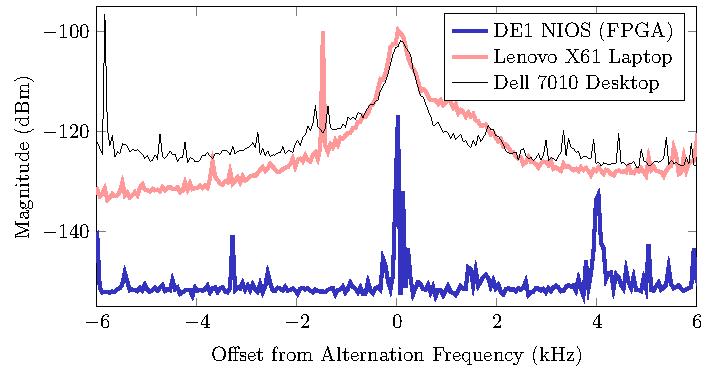
\includegraphics[width=5in]{../emc_comparison_4/spect_cmp.pdf}
\caption{Comparison of power spectra for LDM/LDL1 on DE1 NIOS (FPGA), Lenovo X61 laptop, and Dell 7010 desktop.}
\label{LDM-LDL1-Spectrum}
\end{figure}

It is interesting to observe that the generated signals are almost perfectly concentrated at the intended alternation frequency for the FPGA board, but are much more spread for laptops and desktops. One possible explanation for the wider spectra is that the alternation frequency cannot be controlled perfectly in laptops and desktops and that the alternation period $T$ varies slightly in complex processors, resulting in the dispersion of power around the alternation frequency. This is likely caused by greater variation in the total off-chip memory access time on the desktop and laptop systems. Furthermore, we observe that emanations from desktops and laptops are much stronger than those from FPGA, which aligns with the number of switching transistors and power expended in complex systems. To ensure we are capturing all the power generated by our benchmark, we integrate over the frequency band from $2.5~{\rm kHz}$ below to $2.5~{\rm kHz}$ above the alternation frequency to find the total generated signal power. This power is converted to energy per instruction (SAVAT) according to Equation~\ref{eqn:meas_ese}. 

\begin{table}[htb]
  \scriptsize
  \setlength{\tabcolsep}{2.3pt}
  \setlength\extrarowheight{1pt}
  \caption{SAVAT collected $10~{\rm cm}$ above the NIOS processor on the DE1 FPGA board with the 4cm coil probe. Values are in zepto-Joules.}
  \begin{tabu}{|c||c|c|c|c|c|c|c|c|c|} \hline
    & \textbf{LDM} & \textbf{STM} & \textbf{LDL1} & \textbf{STL1} & \textbf{NOI} & \textbf{ADD} & \textbf{SUB} & \textbf{MUL} & \textbf{DIV}
    \\ \hhline{|=||=|=|=|=|=|=|=|=|=|}
    \textbf{LDM} &  {0.05} &  {1.84} &  {3.77} &  {4.13} &  {4.90} &  {6.22} &  {7.22} &  {3.98} &  {4.02} \\ \hline
    \textbf{STM} &  {1.74} &  {0.03} &  {1.34} &  {1.15} &  {1.33} &  {1.35} &  {1.59} &  {1.31} &  {1.38} \\ \hline
    \textbf{LDL1} &  {3.93} &  {1.47} &  {0.03} &  {0.18} &  {0.66} &  {0.74} &  {1.18} &  {0.05} &  {0.04} \\ \hline
    \textbf{STL1} &  {4.32} &  {1.23} &  {0.20} &  {0.01} &  {0.24} &  {0.22} &  {0.46} &  {0.10} &  {0.24} \\ \hline
    \textbf{NOI} &  {5.11} &  {1.42} &  {0.70} &  {0.26} &  {0.02} &  {0.02} &  {0.07} &  {0.53} &  {0.87} \\ \hline
    \textbf{ADD} &  {5.11} &  {1.40} &  {0.83} &  {0.26} &  {0.02} &  {0.02} &  {0.03} &  {0.68} &  {0.87} \\ \hline
    \textbf{SUB} &  {7.03} &  {1.60} &  {1.05} &  {0.45} &  {0.05} &  {0.07} &  {0.02} &  {1.03} &  {1.25} \\ \hline
    \textbf{MUL} &  {4.10} &  {1.44} &  {0.04} &  {0.09} &  {0.55} &  {0.63} &  {0.95} &  {0.00} &  {0.08} \\ \hline
    \textbf{DIV} &  {4.28} &  {1.54} &  {0.05} &  {0.24} &  {0.91} &  {0.92} &  {1.29} &  {0.08} &  {0.02} \\ \hline

     \end{tabu}

  \label{fig:FPGA}
\end{table}

\begin{table}[htb]
  \scriptsize
  \setlength{\tabcolsep}{2.3pt}
  \setlength\extrarowheight{1pt}
  \caption{SAVAT collected $10~{\rm cm}$ above the Lenovo X61 laptop  with the 4cm coil probe. Values are in zepto-Joules.}
  \begin{tabu}{|c||c|c|c|c|c|c|c|c|c|c|c|} \hline
    & \textbf{LDM} & \textbf{STM} & \textbf{LDL2} & \textbf{STL2} & \textbf{LDL1} & \textbf{STL1} & \textbf{NOI} & \textbf{ADD} & \textbf{SUB} & \textbf{MUL} & \textbf{DIV}
    \\ \hhline{|=||=|=|=|=|=|=|=|=|=|=|=|}
    \textbf{LDM} & {0} & {35} & {182} & {96} & {610} & {661} & {515} & {667} & {659} & {661} & {2160} \\ \hline
    \textbf{STM} & {45} & {0} & {6} & {6} & {21} & {24} & {13} & {18} & {18} & {18} & {130} \\ \hline
    \textbf{LDL2} & {175} & {6} & {0} & {18} & {176} & {195} & {163} & {203} & {200} & {203} & {283} \\ \hline
    \textbf{STL2} & {96} & {11} & {16} & {0} & {263} & {292} & {256} & {301} & {292} & {297} & {363} \\ \hline
    \textbf{LDL1} & {637} & {23} & {191} & {298} & {0} & {0} & {0} & {0} & {0} & {0} & {19} \\ \hline
    \textbf{STL1} & {667} & {45} & {185} & {302} & {0} & {0} & {0} & {0} & {0} & {0} & {15} \\ \hline
    \textbf{NOI} & {536} & {13} & {161} & {262} & {0} & {0} & {0} & {0} & {0} & {0} & {14} \\ \hline
    \textbf{ADD} & {676} & {37} & {193} & {312} & {1} & {0} & {0} & {0} & {0} & {1} & {13} \\ \hline
    \textbf{SUB} & {668} & {23} & {190} & {307} & {1} & {0} & {0} & {0} & {0} & {0} & {18} \\ \hline
    \textbf{MUL} & {677} & {29} & {198} & {310} & {1} & {0} & {0} & {0} & {0} & {0} & {14} \\ \hline
    \textbf{DIV} & {2224} & {176} & {275} & {363} & {19} & {16} &  {14} & {13} & {15} & {14} & {2} \\ \hline
  \end{tabu}

  \label{fig:laptop}
\end{table}


\begin{table}[htb]
  \scriptsize
  \setlength{\tabcolsep}{2.3pt}
  \setlength\extrarowheight{1pt}
  \caption{SAVAT collected $10~{\rm cm}$ above the Dell 7010 desktop with the 4cm coil probe. Values are in zepto-Joules.}
  \begin{tabu}{|c||c|c|c|c|c|c|c|c|c|c|c|} \hline
    & \textbf{LDM} & \textbf{STM} & \textbf{LDL2} & \textbf{STL2} & \textbf{LDL1} & \textbf{STL1} & \textbf{NOI} & \textbf{ADD} & \textbf{SUB} & \textbf{MUL} & \textbf{DIV}
    \\ \hhline{|=||=|=|=|=|=|=|=|=|=|=|=|}
    \textbf{LDM} &  {2} &  {262} &  {84} &  {82} &  {140} &  {170} &  {155} &  {179} &  {196} &  {148} &  {861} \\ \hline
    \textbf{STM} &  {55} &  {1} &  {164} &  {162} &  {306} &  {334} &  {369} &  {420} &  {418} &  {318} &  {1490} \\ \hline
    \textbf{LDL2} &  {85} &  {153} &  {1} &  {1} &  {32} &  {43} &  {43} &  {51} &  {55} &  {42} &  {297} \\ \hline
    \textbf{STL2} &  {84} &  {165} &  {2} &  {1} &  {46} &  {44} &  {85} &  {72} &  {66} &  {33} &  {256} \\ \hline
    \textbf{LDL1} &  {140} &  {296} &  {27} &  {24} &  {0} &  {1} &  {2} &  {3} &  {5} &  {1} &  {108} \\ \hline
    \textbf{STL1} &  {143} &  {321} &  {29} &  {44} &  {0} &  {0} &  {5} &  {4} &  {3} &  {1} &  {61} \\ \hline
    \textbf{NOI} &  {144} &  {332} &  {44} &  {39} &  {2} &  {0} &  {0} &  {0} &  {0} &  {0} &  {76} \\ \hline
    \textbf{ADD} &  {198} &  {423} &  {58} &  {54} &  {5} &  {1} &  {1} &  {1} &  {1} &  {1} &  {60} \\ \hline
    \textbf{SUB} &  {145} &  {321} &  {38} &  {55} &  {1} &  {1} &  {2} &  {1} &  {2} &  {2} &  {48} \\ \hline
    \textbf{MUL} &  {189} &  {431} &  {64} &  {49} &  {7} &  {1} &  {1} &  {2} &  {2} &  {2} &  {59} \\ \hline
    \textbf{DIV} &  {708} &  {1400} &  {193} &  {246} &  {58} &  {56} &  {25} &  {70} &  {31} &  {76} &  {2} \\ \hline

  \end{tabu}
  \label{fig:desktop}
   \end{table}

These tables only describe one possible probe position and orientation, though there are several trends that have been found to be generally consistent across many probe positions and across the tested systems. First, the differences between the ADD, SUB and NOI columns (and rows) is generally within experimental error. This means that adding (or removing) a single integer add or subtract instruction, or substituting an ADD for a SUB has an extremely small impact on emanations. Second, the integer divide instruction generates significantly more SAVAT than the add and subtract operation. This is likely because division is a more complex operation executed over several clock cycles, expending more energy. Finally, regarding loads and stores, more side channel energy per instruction is available to the attacker as higher levels of the memory hierarchy are accessed. In other words, generally L2 cache accesses have higher SAVAT than L1 cache accesses, and memory accesses have higher SAVAT than L1 and L2 cache accesses. This is consistent with the intuition that higher levels of the memory heirarchy should emanate more strongly since such accesses {\it expend} more energy per instruction, activating more circuitry and drawing more current through longer wires (antennas). %Finally, the SAVAT values are in line with the power levels of the processor and system: the FPGA uses less than 2 Watts while the laptop and desktop use greater than 50 Watts, which is consistent with the lower FPGA SAVAT values. 


\subsection{Characterization of SAVAT Reliability and Repeatability}
\label{savat-characterization}

This section uses the measurement setups described in Section~\ref{sec:setup} to illustrate the usefulness and repeatability of the SAVAT metric. It describes general SAVAT properties and demonstrates SAVAT's consistency across repeated measurements on one system as well as between two different systems with the same design. Section~\ref{sec:dutycycle} shows the effect of changing the duty cycle of the benchmark (the time instruction A is active vs the time instruction B is active), and shows that SAVAT does not change significantly if we exchange the order of instructions A and B in the microbenchmarks. Section~\ref{sec:freq} explains the impact of the alternation frequency on SAVAT. %Finally, Section~\ref{sec:distance} shows that SAVAT sources in computer systems can be modelled as a combination of Hertzian and magnetic dipoles and measures SAVAT as a function of measurement distance.

Practical usage of SAVAT requires that measurements taken on a single system are repeatable and consistent (precise). The tables in section~\ref{savat-20cm} showed the SAVAT values for 4 laptops and desktops. To generate these tables, SAVAT was measured 10 times for each instruction pair at a $80~{\rm kHz}$ alternation frequency and at a distance of $10~{\rm cm}$, measured on the four tested computer systems in Table~\ref{pc_specs}. The tables in Section~\ref{savat-20cm} show the means of each set of measurements for a given A/B instruction pair. Figure~\ref{fig:Variation} plots these means, along with the standard deviation among the 10 repeated measurements of each A/B instruction pair. Each point indicates the mean and standard deviation of one population of 10 SAVAT measurements (i.e. one entry in Table~\ref{fig:savat-20cm-lx61}). The position along the $x$-axis represents the mean and the $y$-axis position indicates the standard deviation for each SAVAT value. The precision is good (stdev/mean $<$ 10\%), so the resulting SAVAT values can be used to guide design decisions with confidence. This also implies that our measurements are repeatable, and indicates that the signal created by the alternation loop (discussed in the previous paragraph) is the dominant source of error in the measured SAVAT values.

\begin{figure}[htb]
  \centering
  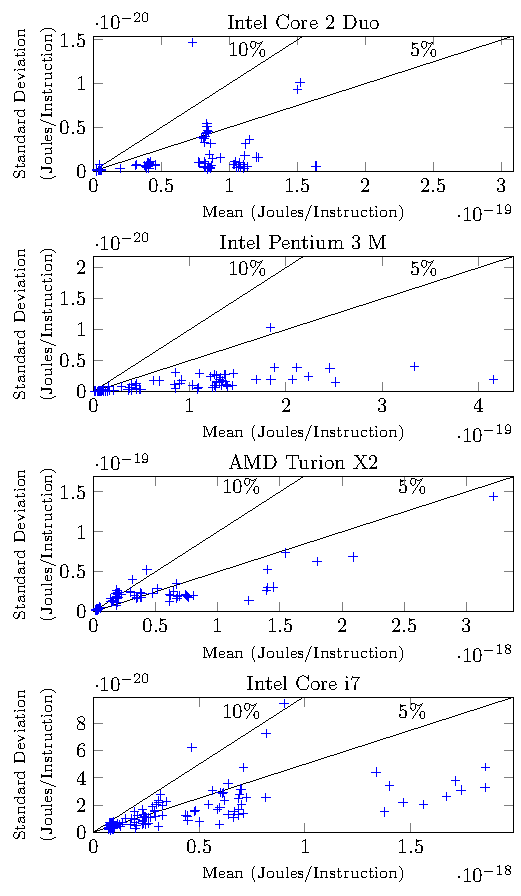
\includegraphics[width=3in]{../TEMC_SAVAT/figures/variation.pdf}
  \caption{SAVAT measurement precision.}
  \label{fig:Variation}
\end{figure}

SAVAT values must also be consistent between different physical units of the same system design for SAVAT to be practical. Figure~\ref{fig:2PCs} compares SAVAT values from two PCs (2 physical units of a DELL Optiplex 7010 model with Core i7 processors) for three different alternation frequencies using the 20 cm loop antenna. For each alternation frequency and PC, the SAVAT values have been separately normalized by the equation $\textrm{SAVAT}_{plot} = \textrm{SAVAT}_{measured}/\mu_{A/B}$ %, where $\mu_{A/A}$ is the mean of all A/A measurements (diagonal entries in Figure~\ref{fig:C2D-10-80-Table})
where $\mu_{A/B}$ is the mean of all A/B measurements where A and B are different (i.e. the off-diagonal entries in Table~\ref{fig:savat-20cm-d7010}). The black line corresponds to a perfect 1-to-1 match, and the closeness of the data points to this line indicates there is a good match between the two systems for all three alternation frequencies. This implies that SAVAT values measured on one physical system can represent all manufactured systems of the same or similar design and that our measured SAVAT values are largely insensitive to the alternation frequency.

\begin{figure}[htb]
  \centering%
  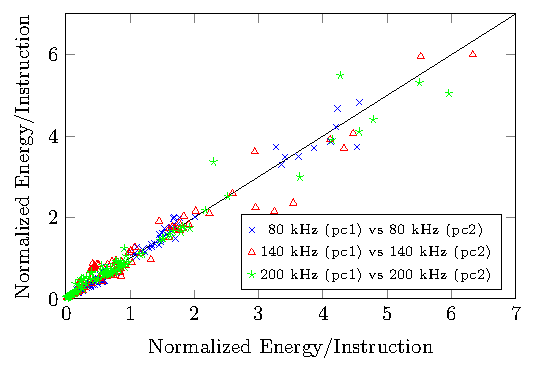
\includegraphics[width=5in]{../TEMC_SAVAT/figures/two_pcs.pdf}
  \caption{SAVAT comparison for two identical desktop (DELL Optiplex 7010) systems.}%
  \label{fig:2PCs}
\end{figure}

\subsubsection{Impact of A/B Duty Cycle and Instruction Ordering}\label{sec:dutycycle}

When measuring SAVAT the A and B instructions are each executed the same number of times per each loop iteration (\texttt{n\_inst}) because this allows us to directly calculate the energy per each executed instruction using the derivation in Appendix~\ref{appendix}. However, it is also possible to execute more A instructions than B instructions or vice versa. This changes the duty cycle for the $w[n]$ waveform described in Appendix~\ref{appendix}. Changing this duty cycle changes the magnitude of $W[1]$ and therefore changes the magnitude of $V[1]$ and the measured spectral power. 

\begin{figure}[htb]
\centering
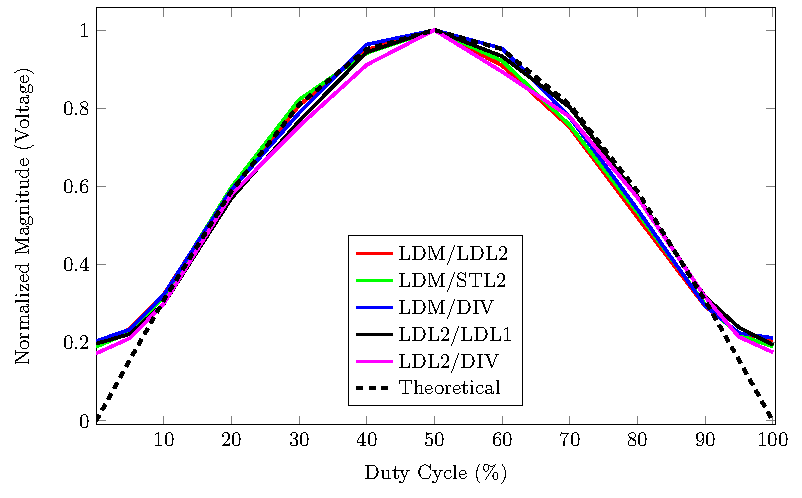
\includegraphics[width=5in]{../TEMC_SAVAT/duty_fit.pdf}
\caption{The effect of the alternation waveform duty cycle on observed SAVAT.}
\label{duty_fit}
\end{figure}

The effect of the duty cycle on different pairs of instructions is illustrated in Figure~\ref{duty_fit}. These results were obtained by varying the duty cycle of several A/B pairs and observing the change in power as a function of duty cycle. The duty cycle was varied by executing the A and B instructions different numbers of times per each iteration of the alternation loop. For example, if executing LDL1 and LDL2 $100$ times each per loop iteration results in a duty cycle of $50\%$, then executing LDL1 50 times and LDL2 150 times per iteration results in a duty cycle of $25\%$. Each instruction pair has a different maximum magnitude (as seen in the SAVAT tables) and so the general trend is best seen by normalizing each curve so that the power observed at $50\%$ duty cycle is plotted at 1.

These experimental values can be compared against the theoretical curve using Fourier analysis of square waves with varying duty cycle. From Fourier analysis the amplitude of the first harmonic of the rectangular wave $w[n]$ (for large $n_{inst}$) is~\cite{smith1997}
\begin{equation} \label{duty_fourier}
\frac{W[1]}{2Nn_{inst}} \approx \frac{1}{\pi}\sin(\frac{\pi \tau}{T})
\end{equation}
where $w[n]$ is 1 (i.e. instruction A is active) for time $\tau$ and 0 (i.e. instruction B is active) for time $T-\tau$. $\tau/T$ is the duty cycle. Using Equation~\ref{eqn:P_f_alt} and normalizing so that the amplitude of the first harmonic at 50\% duty cycle is 1 (to match the normalized measurements just described), in theory the measured magnitude should vary as a function of duty cycle as $\sin(\frac{\pi \tau}{T})$. This theoretical result is shown as a dotted black line in Figure~\ref{duty_fit}.

Previously we also claimed that the SAVAT tables are generally symmetric. In other words, $\textrm{SAVAT}(A,B) \approx \textrm{SAVAT}(B,A)$. To test this, we measured SAVAT for several A/B and B/A pairs at three different frequencies ($80~{\rm kHz}$, $140~{\rm kHz}$, and $200~{\rm kHz}$) on the DELL Optiplex 7010 desktop with the 20 cm loop antenna as shown in Figure~\ref{fig:Order}. The black line corresponds to a perfect 1-to-1 match. Instruction ordering creates only small deviations from the perfect match for all three alternation frequencies which implies that the ordering of instructions does not significantly impact the measured SAVAT.
\begin{figure}[htb]
	\centering
	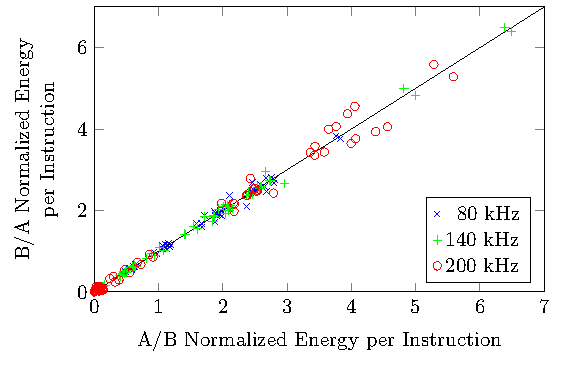
\includegraphics[width=5in]{../TEMC_SAVAT/figures/ab_vs_ba.pdf}
	\caption{ The effect of instruction ordering on observed SAVAT.\label{fig:Order}}
\end{figure}

\subsection{Impact of the Alternation Frequency}\label{sec:freq}

The power spectrum measured close to a desktop or laptop computer consists of numerous peaks protruding above ``rolling hills'' of noise. In addition to intentional radio signals (such as Wifi and Bluetooth), each system has numerous other emanations sources. Switching power supplies create broad noise peaks, clocks create narrow peaks at their operating frequency, and long cables radiate noise across a broad range of frequencies. In addition, moving an EM probe closer to the test system ($<$ 1 meter) reveals that the random switching activities in the processor and other system components create a broadband noise floor (typically higher than the spectrum analyzer noise floor) that varies as a function of frequency.

SAVAT integrates spectral power density over a frequency band around the alternation frequency (5 kHz bandwidth in our experiments), so measuring the same SAVAT value at different alternation frequencies will unavoidably integrate different noise sources along with the intended signal, resulting in different SAVAT values. The emanations created by our benchmarks at the alternation frequency are likely caused by currents flowing through the system's power distribution network (PDN) and are therefore a function of the path this current takes through the PDN. The PDN can be modelled as a network of shunt capacitances and series inductances, and so the current's path is expected to be frequency dependent. A longer current path might enclose a loop with a larger area, creating stronger emanations~\cite{Ott09}. To account for this frequency dependent ``gain'' we normalize by the average SAVAT value at a given frequency when comparing SAVAT across frequencies. For neighboring frequencies (e.g. 80kHz vs 90kHz or 190kHz vs 200kHz), the change in gain is small as shown in Figure~\ref{fig:fdepend} for the DELL Optiplex 7010 desktop with the 20 cm loop antenna. %is this DELL?

\begin{figure}[htb]
	\centering
	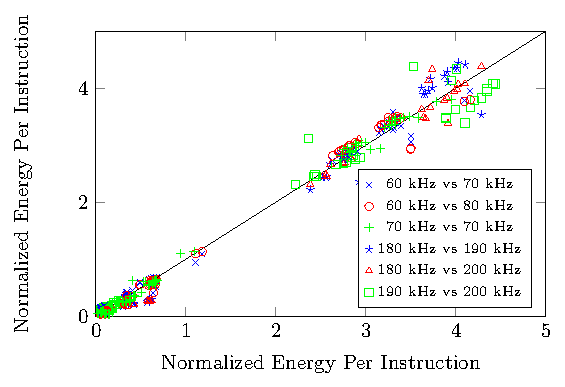
\includegraphics[width=5in]{../TEMC_SAVAT/fdepend.pdf}
	\caption{Comparison of SAVAT at different frequencies for the DELL Optiplex 7010 desktop.}
  \label{fig:fdepend}  
\end{figure}

\begin{figure}[htb]
	\centering
	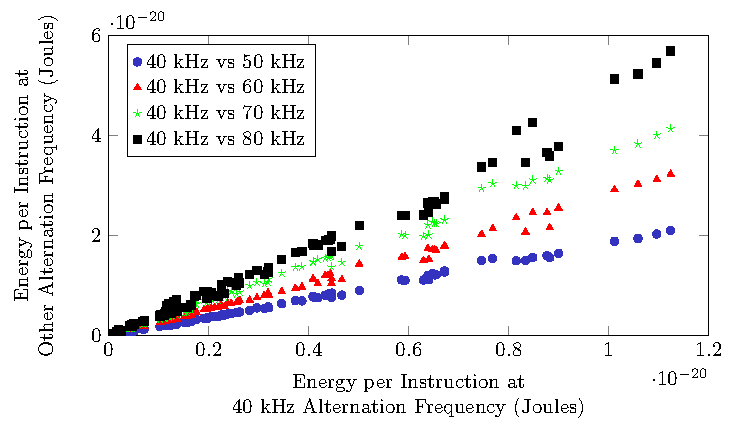
\includegraphics[width=5in]{../emc_comparison_4/freq_depend.pdf}
	\caption{Comparison of SAVATs at different frequencies for NIOS on the DE1 FPGA board. }
  \label{fig:fdepend_nios}
\end{figure}

\begin{figure}[hbt]
	\centering
	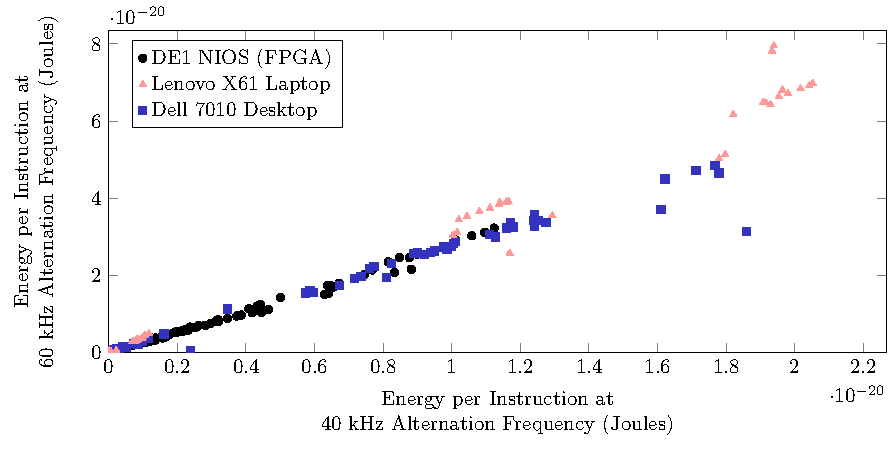
\includegraphics[width=\textwidth]{../emc_comparison_4/freq_depend_compare.pdf}
	\caption{Comparison of SAVATs at 40 kHz and 60 kHz for the NIOS DE1 FPGA, the Lenovo X61 laptop, and the DELL Optiplex 7010 desktop.}   \label{fig:fdepend_compare}
\end{figure}


Figure~\ref{fig:fdepend_nios} shows how SAVAT changes as a function of the alternation frequency on NIOS measured with the 4cm coil probe.% this figure is technically not showing the effect of gain
Each instruction pair is plotted along the x-axis at its SAVAT value measured at 40 kHz, and is plotted along the y-axis at its SAVAT value measured at another frequency. The SAVAT values at 40 kHz appear to be linearly related to the SAVAT values at each other frequency, suggesting that SAVAT values at one frequency can be used to predict SAVAT values at any other frequency in this range. Therefore within this frequency range the DE1 NIOS SAVAT is largely independent of frequency and can be measured at whichever frequency is most convenient. Figure~\ref{fig:fdepend_compare} shows the FPGA SAVAT values at 40 kHz vs 60 kHz, along with the laptop and desktop SAVAT values of comparable magnitude at the same frequencies. All three systems follow a similar trend, suggesting that the SAVAT values on all three systems may have a similar dependence on the measurement frequency.


\begin{comment}
\subsection{Modeling SAVAT Power as a Function of Distance}\label{sec:distance}

To model the sources of these EM emanations and to estimate how far away EM emanations can be received, we need to know how quickly SAVAT decays with distance. Since we are measuring near-field signals using a magnetic loop probe, we expect that the magnetic field will decay as $1/{r^3}$ and that the emanations source can be modelled as a magnetic dipole. However, our measurements did not match this model. Hence, we modelled the side-channel field as a field created by an electric monopole (Hertzian dipole) and a magnetic dipole, where we can receive only magnetic components of the EM field. Hence, the received power can be modelled as
\begin{equation}
	P_r  = {P_t}'\left(\frac{1}{(kr^2)^2}+\frac{1}{(kr^3)^2}\right)
\end{equation}
where \begin{math} k={2\pi}/{\lambda} \end{math} is the wavenumber, \begin{math} {P_t}' \end{math} is a fixed constant to align each theoretical curve to the corresponding power measurement at $0.25$ meters, and $r$ is the distance between the antenna and the system. Figure~\ref{fig:distance} compares theoretical and measured SAVAT for several representative instructions measured at $215~{\rm kHz}$. We observe that the received power of on-chip pairs of instructions (e.g. LDL2/DIV and LDL2/LDL1) decays at the same rate as the received power on-chip/off-chip instruction pairs (e.g. LDL2/STM). Similar agreement between theoretical and measured SAVAT was found at $70~{\rm kHz}$ and $150~{\rm kHz}$.
% using a different r to account for different on-chip and off-chip distance(?)
% mention that this was Core 2 Duo Laptop?
% explain that chose 215 kHz since it had largest magnitude (longest distance)?
% since measurement is normalized at 25cm, the effect of k is cancelled out

\begin{figure}[htb]
	\centering
	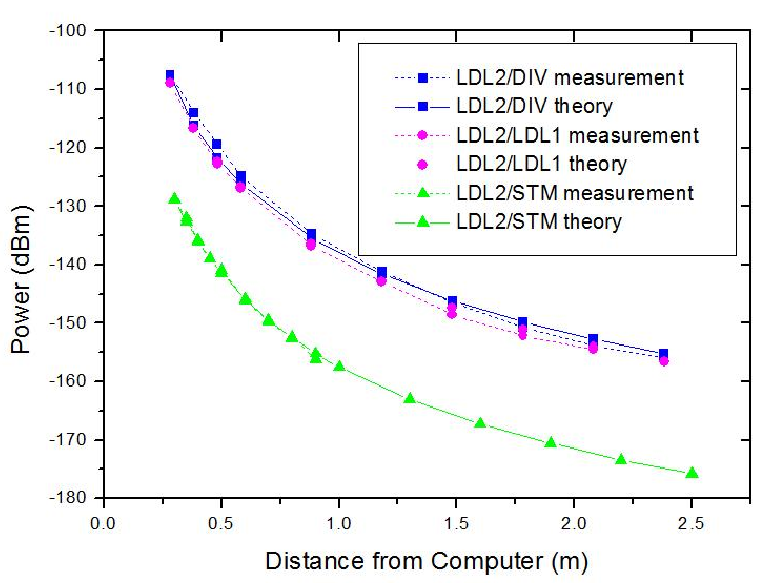
\includegraphics[width=5in]{../TEMC_SAVAT/distance1.pdf}
	\caption{SAVAT as a function of measurement distance.}
\label{fig:distance}    
\end{figure}
\end{comment}


\section{Summary}

%Side channels enable a powerful class of attacks that circumvent traditional protections, and a significant number of such attacks and potential countermeasures have been proposed for both hardware and software. Recent work has shown that potential side channel vulnerability can be assessed at the level of an entire processor or system, and at the granularity of entire phases. However, without a practical way to attribute potential side channel vulnerability to specific instruction-level behavior, it is difficult for computer architects and software developers to apply countermeasures strategically to limit their cost and performance/power impact.

This chapter presented a new metric, which we call \SAVATfull (SAVAT), that measures the side channel signal created by a specific single-instruction difference in program execution, i.e. the amount of signal made available to a potential attacker who wishes to decide whether the program has executed instruction/event A or instruction/event B. We also devised a practical methodology for measuring SAVAT in real systems using only user-level access permissions and realistic measurement equipment. While similar metrics rely on time domain measurements, SAVAT is measured in the frequency domain, overcoming some challenges posed by time domain measurements of EM emanations caused by instruction execution in high performance systems. 

We measured SAVAT among several common x86 instructions on three different laptops and one desktop at several different frequencies. Our results showed that two systems with the same design have nearly identical measured SAVAT values, which implies that SAVAT measurements on one system are representative of an entire manufacturing run, or possibly an entire family, of systems. Our SAVAT measurements were precise (st.dev/mean $<$ 5\%) for each tested system. We also demonstrated that SAVAT measurements are consistent regardless of instruction order and other implementation details. We also measured the effect of unequal A and B instruction counts and showed that with appropriate normalization, SAVAT is consistent over a range of frequencies. % and we showed that the sources of EM side-channel emanations in computer systems can be modelled as a combination of Hertzian and magnetic dipoles and showed how SAVAT decays as a function of distance.
Finally, to illustrate the validity of SAVAT we derived a relationship between SAVAT and a simple time domain metric. 



Overall, we confirmed that our new metric and methodology can help discover the highest-vulnerability aspects of a processor architecture or a program, and thus inform decision-making about how to best manage the overall side channel vulnerability of a processor, program, or system. SAVAT can be used by circuit designers and microarchitects to reduce susceptibility to side channel attacks by focusing on high-SAVAT aspects of their designs (e.g. off-chip memory accesses, last-level-cache hits, and possibly the integer divider in the systems we measured). Programmers, compilers, and algorithm designers can also use SAVAT to guide code changes to avoid using ``loud'' activity when operating on sensitive data. Overall, our instruction-level metric and methodology differ from prior work in that they {\em quantify} the signal that is sent to the attacker by an {\em instruction-level difference} in program execution. These measurements can be used to determine the potential for information leakage when execution of individual instructions or even sections of code depends on sensitive information. We expect our instruction-level attribution of potential side channel vulnerability to help system designers decide {\em where in the system/processor} to apply countermeasures, and also to help programmers and compilers apply software-based countermeasures selectively to minimize their performance and power impact.


%\section{SAVAT EM vs Power}
%\input{savat-em-vs-power}

\chapter{FASE: Finding Amplitude-modulated Side-channel Emanations}
\label{sec:fase}
\section{Overview}
This chapter describes FASE (Finding Amplitude-modulated Side-channel Emanations). FASE systematically and efficiently identifies periodic EM emanations whose amplitudes change as a result of specific changes in system activity, i.e. signals that are amplitude-modulated by system activity. Our methodology uses the SAVAT micro-benchmarks to generate repetitive changes in processor and memory activity, then processes the resulting EM signals to find spectral patterns corresponding to amplitude modulation. The EM spectrum is full of amplitude-modulated signals (e.g. radio broadcasts) that are not modulated by program activity. FASE filters out such signals by generating several different activity patterns and reporting only those signals which are specifically modulated by all the generated activity patterns. 

Side channels based on physical side-effects (power consumption, sound, or EM emanations) are difficult for microarchitects and programmers to alleviate, in part because the relationship between computational behavior and the resulting side channel signal is very complex and poorly understood. EM emanations side channels may be the most complex: the emanated signals may theoretically be anywhere in the EM spectrum, and signals at different frequencies may provide attackers with insight into different aspects of computational activity.  Therefore, the first step to use or mitigate side channel leakage is to identify signals that have some dependence on the secret information of interest. Much previous work addresses finding leakage signals as part of the process of carrying out an attack~\cite{Kocher99,gebotys2005,meynard2011,sugawara2009}. However, many of these side channel attack descriptions only briefly or implicitly address the underlying mechanisms that cause information leakage. While attacks do not require determining the cause of leakage, efficient mitigation does. Without a systematic approach to identification and causation, the process of finding root causes is time-consuming and mostly trial-and-error: the defender makes an educated guess about the leakage source, fixes the hypothesized problem, and sees whether the leakage has been reduced.

The FASE approach for discovering AM-modulated signals is highly effective at both finding modulated leakage sources, and at determining the type of activities causing the leakage. Computer systems generate thousands of periodic EM emanations. FASE successfully rejects all such signals that are not modulated by system activity, while reporting the small number of remaining signals that are modulated by specific system activities. This chapter describes unintentional AM modulated signals in computer systems, and then describes how FASE can be used to find and characterize such signals. To test FASE, we use it to find AM signals on a number of different computer systems. We also identify the source of each periodic signal and the mechanism by which it was modulated to demonstrate the usefulness of FASE and to understand potential EM side-channel vulnerabilities of modern processor and memory systems. Finally, we present a fully automated version of FASE and use it to find AM modulated signals on a large range of devices.


\section{Unintentional AM Carriers in Computer Systems}
\label{sec:fase-am-devices}
Amplitude modulation (AM) is well-studied~\cite{rappaport} and is used in numerous communications systems. AM communications rely on carefully designed transmitters and thoroughly regulated allocation of the frequency spectrum to minimize interference. Unintentional AM signals in computer systems are generated by many possible ``transmitters.'' A memory clock signal, for example, may act as a carrier. A clock signal creates periodic currents at the clock frequency $f_c$, and these currents flow through power and signal wires, generating a strong EM field. When the memory is active, more current is drawn by the clock, and less current is drawn when the memory is less active. If we alternate between high memory activity and low memory activity with a frequency $f_{alt}$, the amplitude of the carrier at $f_c$ is modulated creating signals at $f_c \pm f_{alt}$.

The transmission and reception of such unintentional modulation ``signals'' differ from communication signals in several ways. Since unintentional signals occur at the frequency of the unintentional carrier, they are mixed in with all the other noise generated by the computer system (other clocks and switching noise) and other communications signals. Unintentional signals are subject to EMC restrictions which impose a maximum noise power (signal power from our point of view). Therefore, unintentional signals are typically weaker and may be diffused across the spectrum by spread spectrum clocking or by using clock sources with inherent variation (e.g. RC oscillators). Also, since the carriers are typically generated by non-sinusoidal sources, the carrier signals may have harmonics.

These effects complicate the detection of unintentionally modulated signals. The presence of noise generated by the system makes it difficult to determine which signals are AM carriers and sidebands. Some of the unintentional AM carriers are generated by spread spectrum clocked signals, making them harder to recognize. Existing methods to find AM modulation based on its spectral properties (i.e. without knowing the baseband signals) are not designed to deal with these issues.

Finally, communication signals have direct and obvious control of the baseband (modulation) signal while unintentionally modulated signals from computer systems do not. In some cases, multiple baseband signals may even modulate the same unintentional carrier present in a computing system. We may, for example, be interested in separating out and determining the source of each such baseband signal (i.e. a particular system activity). For example, a baseband signal may be caused by processor activity and another baseband signal may be caused by memory activity. Existing AM detection methods are not able to identify which carriers are modulated by specific system activities.

The spectral properties of amplitude modulated non-ideal carriers are summarized in Section~\ref{am_spectra}. Several other non-ideal properties of computer systems are seen in measured spectra. Randomly timed switching activity causes broadband noise, and this noise appears as gently rolling ``hills'' and ``valleys'' in the spectrum. Additionally, a realistic spectrum contains periodic signals from both inside and outside the system that are either not modulated at all or that \emph{are} AM-modulated (e.g. AM radio broadcasting) but not by program activity. Such a spectrum is shown in Figure~\ref{am_details_e}. Even if we know the carrier and the program activity's frequency content it is hard to decide whether this spectrum contains an activity-modulated signal by visual inspection. Our FASE methodology uses several specially generated program activities in conjunction with a heuristic carrier likelihood
%\footnote{Likelihood here does not refer to probability estimates.}
function to automate the decision process and overcome these problems.

\begin{figure}[thb]
  \centering
    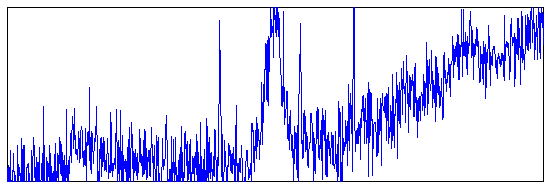
\includegraphics[scale=.95]{../fase/Data/am_details_e.pdf}
  \caption{The same non-ideal carrier and arbitrary side-band signal as Figure~\ref{am_details_d} with noise and other sources present.}
  \label{am_details_e}
\end{figure}

Many periodic carrier signals in computer systems are generated by digital circuits and clocks, and therefore have sharp transitions that are best approximated by rectangular pulses instead of the sinusoidal waves used as carriers in communications systems. The spectrum of a pulse train with an arbitrary duty cycle is equivalent via Fourier analysis to a set of sinusoids with various amplitudes at $f_c$ and its multiples (harmonics). 
In other words, for each carrier signal generated by a digital circuit or clock, additional carrier signals will also be present at $2f_c$, $3f_c$, $4f_c$, $5f_c$, etc. As the duty cycle of a signal approaches 50\%, the amplitudes of the odd-numbered harmonics ($f_c$, $3f_c$, $5f_c$, etc.) reach their maximum, while amplitudes of the even harmonics ($2f_c$, $4f_c$, etc) trend toward zero. For a small duty cycle (i.e. $<$ 10\%), the magnitudes of the first few harmonics (both even and odd) decay approximately linearly. Finally, note that these observations imply that the amplitudes of all the harmonics are a function of the duty cycle. If program activity modulates the duty cycle of a periodic signal while keeping its period constant (i.e. causes pulse width modulation), all of the signal's harmonics are amplitude-modulated and consequently will be identified by our FASE methodology.



\section{Methodology for FASE}
\label{sec:fase-methodology}
A carrier at frequency $f_c$ modulated by system activity is a lot easier to recognize if we generate periodic processor and/or memory activity that repeats $f_{alt}$ times per second. We will used the SAVAT micro-benchmarks (which create measurable periodic signals at arbitrary frequencies as described in Chapter~\ref{sec:savat}) to find AM modulated signals in computer systems. A modified version of one such micro-benchmark is shown in Figure~\ref{fase_pseudocode}. Recall that the loop beginning on line \ref{BegLoopA_fase} performs one activity (activity A), and the loop beginning on line~\ref{BegLoopB_fase} performs another activity (activity B). The outer loop repeatedly alternates activities A and B, creating periodically changing activity whose period equals the execution time for one iteration of the outer loop. This alternation period $T_{alt}$ is the inverse of the frequency $f_{alt} = \frac{1}{T_{alt}}$. Note that in Chapter~\ref{sec:savat}, we used this alternation to \emph{generate a carrier signal} at some chosen frequency $f_c$, while in this chapter we use this alternation at $f_{alt}$ to measure AM-modulation of any potential \emph{carrier signals intrinsically generated} (and emanated) by the system.

\begin{figure}[htb]
\lstset{language=C++,basicstyle=\ttfamily\footnotesize,numbers=left}\lstset{escapeinside={/*@}{@*/}}
\begin{lstlisting}[frame=none,xleftmargin=30pt]
while(true){/*@\label{BegInfLoop_fase}@*/
  // Execute the A activity /*@\label{BegLoopA_fase}@*/
  for(i=0;i<inst_a_count;i++){
    ptr1=(ptr1&~mask1)|((ptr1+offset)&mask1);/*@\label{UpdAddrA_fase}@*/
    // The A-instruction, e.g. a load from L2
    value=*ptr1;/*@\label{TestInstA_fase}@*/
  }/*@\label{EndLoopA_fase}@*/
  // Execute the B activity /*@\label{BegLoopB_fase}@*/
  for(i=0;i<inst_b_count;i++){
    ptr2=(ptr2&~mask2)|((ptr2+offset)&mask2);/*@\label{UpdAddrB_fase}@*/
    // The B-instruction, e.g a store from L2
    *ptr2=value;/*@\label{TestInstB_fase}@*/
  }/*@\label{EndLoopB_fase}@*/
}
\end{lstlisting}
\caption{Pseudo-code to generate the A/B alternation activity.}
\label{fase_pseudocode}
\end{figure}


As an example of how the alternation of activity can AM-modulate a carrier signal, consider a DRAM memory clock signal as shown in Figure~\ref{fig:alt_freq}. Activity A may involve many LLC misses, so it results in substantial DRAM activity. During the A-activity half-period, the DRAM clock drives a lot of switching activity (current flowing through wires), resulting in strong emanations at the DRAM clock frequency. If activity B has little DRAM activity, less switching activity is driven by the DRAM clock, generating weaker emanations at the DRAM clock frequency. Therefore the amplitude of the emanations at the DRAM clock frequency will change with period $T_{alt}$ (frequency $f_{alt}$), which means that emanations at the DRAM clock frequency will be AM-modulated by the A/B periodic behavior whose frequency is $f_{alt}$.

\begin{figure}[tbh]
  \centering
  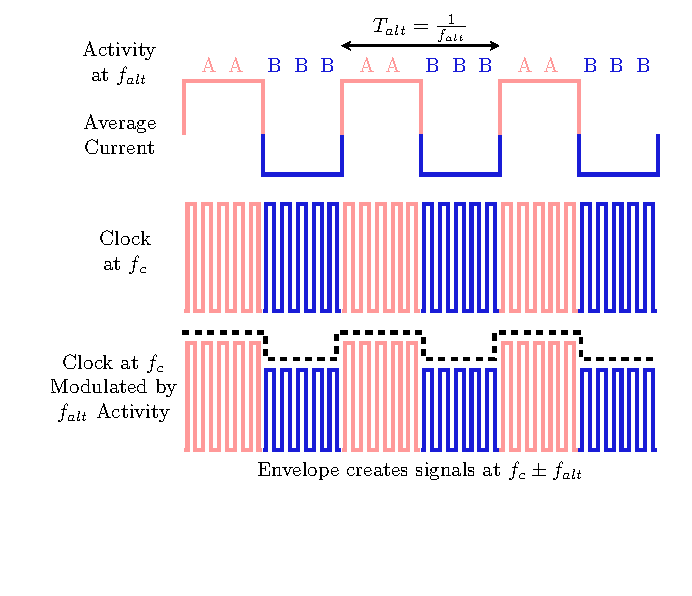
\includegraphics[width=5in]{../fase/Drawing/alt_freq.pdf}
  \caption{The micro-benchmarks do each of activities A and activity B for half the alternation period, resulting in a periodic component at the alternation frequency $f_{alt}$.}
  \label{fig:alt_freq}
\end{figure}

The key difference between the code shown in Figure~\ref{fase_pseudocode} and the SAVAT benchmarks described in Chapter~\ref{sec:savat} is that while the instruction counts for the A and B instructions were equal for SAVAT, for FASE we adjust the \texttt{inst\_a\_count} and \texttt{inst\_b\_count} variables so that activity A and activity B are each done for half of the alternation period (50\% duty cycle). Thus the spectrum of each side-band around the carrier's frequency $f_c$ will also have strong odd-numbered harmonics of the alternation frequency, i.e. the side-band signal will have spikes/peaks at $f_c \pm 3f_{alt}$, $f_c \pm 5f_{alt}$, etc. in addition to $f_c \pm f_{alt}$. Also note that the alternation frequency $f_{alt}$ can be controlled by changing the instruction counts, allowing us to create several separate spectra with sideband signals at different $f_{alt}$ frequencies. These spectra can be considered jointly in an effort to distinguish which carriers are modulated by a particular activity.

Finally, we use loads from memory (LDM), loads from the L2 cache (LDL2), and loads from the L1 cache (LDL1) as the activities A and B in the experiments we report. We have performed additional experiments with other activities (various arithmetic instructions) and have found that for the systems tested such activities modulate the same carriers that on-chip cache accesses do, so we use cache accesses as representatives of on-chip activity. Varying only the memory accesses in our code also allows us to eliminate all other code in the alternation loop as a possible source of modulation -- the address computation for all three types of memory accesses only differs in the values of the \texttt{mask1} and \texttt{mask2} parameters and the memory access instruction itself is also identical in all three cases.

FASE results for different A/B pairings usually provide a strong indication of which aspect of the system modulates a given carrier signal. For example, when a signal at a particular frequency $f_c$ is modulated by A/B alternation between memory activity and any on-chip activity, but remains unmodulated when alternating between two types of on-chip activity, the carrier signal and/or its modulation mechanism are likely related to the memory controller, processor-memory communication, or the DRAM memory itself.

As indicated in Section~\ref{sec:fase-am-devices}, discovery of activity-modulated carriers by ``eyeballing'' the spectrum without generating controlled system activity would be very difficult. Theoretically, one could look for narrow spikes (potential carriers) with symmetric side-bands on either side as shown in Figure~\ref{am_details_b}, but this approach is not practical due to the non-ideal nature of unintentional carriers, the interference of other signals, and noise as shown in Figure~\ref{am_details_e}.

\begin{figure*}[tb]
  \centering
    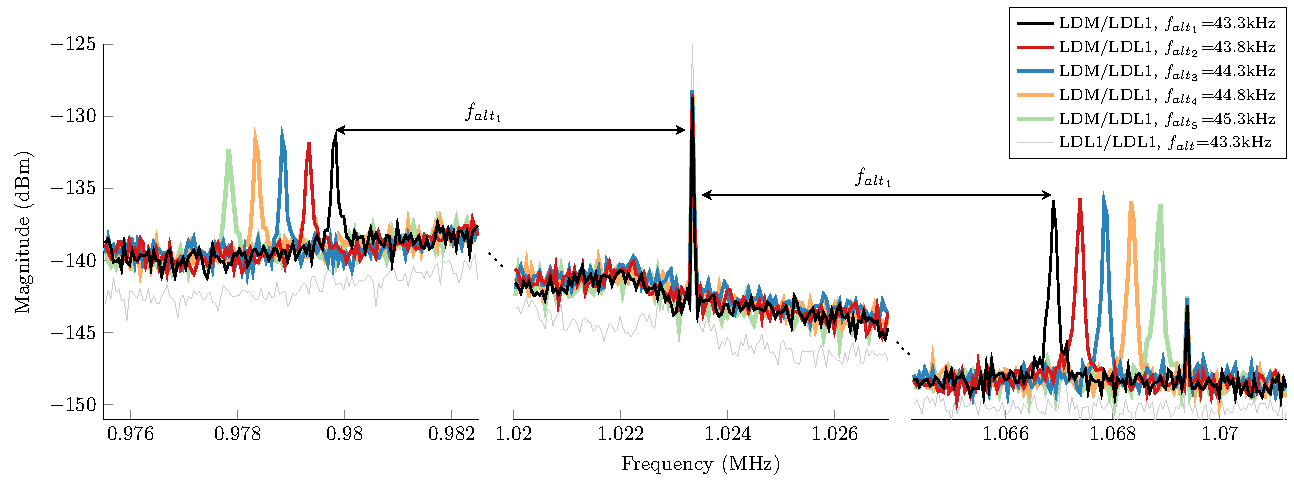
\includegraphics[width=\textwidth]{../fase/Data/mem_refresh_zoom.pdf}
  \caption{A carrier at $f_c$ and its right and left side-bands generated by memory activity.}
  \label{mem_refresh_zoom}
\end{figure*}

Measuring arbitrary programs or benchmarks may provide some information about carriers that are modulated by system activity but it would be difficult to determine the spectral properties of such arbitrary system activity. Even if we are somehow given spectral information about activity in an application, it would be hard to recognize whether the side-band signals around each potential carrier match that spectrum with high confidence because 1) amplitude modulation combines (convolves) the spectrum of the possibly non-ideal carrier signal with the arbitrary benchmark spectrum (Figure~\ref{am_details_d}), and 2) recognition of such a complicated overall spectrum is further hampered by noise and unrelated signals that overlap with portions of the modulated-signal spectrum (Figure~\ref{am_details_e}).
%
We cannot directly control the shape of a system's intrinsic carrier signals, but we can use SAVAT to generate system activity that is as close to a perfect square wave as possible. This results in side-band signals whose spectrum has a shape that closely matches the shape of the carrier signal they are modulating, with a $f_{alt}$ separation between the carrier and its two side-bands in the spectrum. This could be used to find carriers automatically by looking for such right and left side-band signals because they always appear as peaks in the spectrum separated by $2f_{alt}$ with the carrier peak half-way between them. However, this simplistic approach has a number of drawbacks. First, the alternation activity is a square wave which has many odd-numbered harmonics ($f_c \pm f_{alt}$, $f_c \pm 3f_{alt}$, etc.) that are separated by exactly $2f_{alt}$. This makes it difficult to attribute the spikes in the side-band signals to particular carrier frequencies, creating many false positive indications of carrier locations. Second, for some values of $f_{alt}$, some of the side-band signals may be overwhelmed by noise and unrelated signals, which would result in many false negatives. Third, computer systems contain many components with periodic activity, so unmodulated signals are often concentrated at specific frequencies. Some such spectral peaks will be nearly $2f_{alt}$ apart by random chance, resulting in more false positives.

Many of the problems caused by the harmonics of the alternation signal and by the existence of unrelated signals can be solved by performing multiple measurements with different alternation frequencies, e.g. $f_{alt_1}$, $f_{alt_2}=f_{alt_1}+f_\Delta$, $f_{alt_3}=f_{alt_1}+2f_\Delta$, etc., where $f_\Delta$ is typically small compared to $f_{alt}$. Figure~\ref{ideal_fase} illustrates an idealized diagram of the $f_{alt_N}$ side-bands with five such alternation frequencies. Figure~\ref{mem_refresh_zoom} shows five real spectra spectra with $f_{alt_1} = $ 43.3kHz and $f_\Delta = $ 0.5kHz around a carrier signal at $f_c =$ 1.0235MHz. To avoid clutter, Figure~\ref{mem_refresh_zoom} only shows the three parts of the spectrum that contain the left side-bands, the carrier, and the right side-bands of the signals. In other words, it does not show about 40kHz worth of spectrum to the left and right of the carrier. Note how the peaks in the side-bands move by $f_\Delta$ as the alternation frequency $f_{alt}$ changes by $f_\Delta$.

\begin{figure}[tbh]
  \centering
    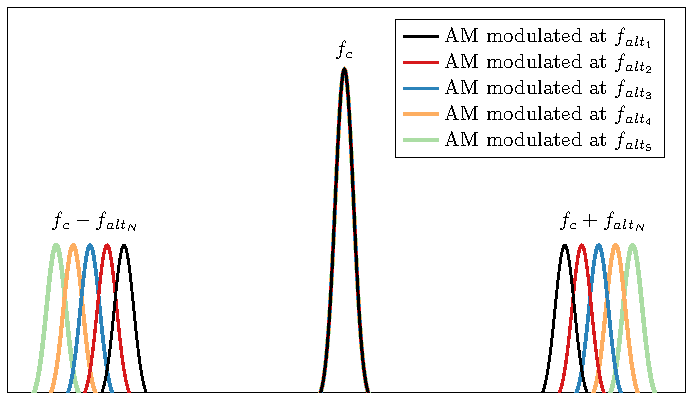
\includegraphics[width=\textwidth]{../fase/Data/ideal_fase.pdf}
  \caption{Ideal FASE spectral pattern illustrating an AM carrier at $f_c$.}
  \label{ideal_fase}
\end{figure}

Conceptually, the FASE methodology for finding activity-modulated carriers and determining the frequencies of such carriers is now as follows. First, perform several measurements (we use five) with different $f_{alt}$ frequencies as described above. Second, look for a shape in the spectrum that moves by $f_\Delta$ or $-f_\Delta$ in successive measurements. This approach eliminates external signals and system-emanated periodic signals that do not correspond to activity-induced AM modulation because such signals stay at the same frequency as $f_{alt}$ changes. It also only detects the first harmonic of $f_{alt}$ to the right and left of the carrier. Recall that the alternation activity changes abruptly and may not have a perfect 50\% duty cycle, so the spectrum of the modulated signal has side-band signals not only at $f_c \pm f_{alt}$ but also at $f_c \pm 2f_{alt}$, $f_c \pm 3f_{alt}$, etc. However, only the first harmonic ($f_c \pm f_{alt}$) moves by $f_\Delta$ in the spectrum as we change $f_{alt}$ by $f_\Delta$. The other harmonics in the side-band move by $2f_\Delta$, $3f_\Delta$, etc.

Once we have identified a first harmonic side-band signal in this way, we can determine whether it is the left side-band (moves by $-f_\Delta$) or the right one (moves by $f_\Delta$), and we can compute the frequency of its carrier signal. The carrier is located at $f - f_{alt_i}$ if the modulated peaks are detected at frequency $f$ and if $f_{alt_1}$ is to the left of $f_{alt_5}$ (or at $f+f_{alt_i}$ if $f_{alt_1}$ is to the right of $f_{alt_5}$). Note that detection of a single harmonic of $f_{alt}$ in a single side-band is sufficient to detect a carrier frequency, i.e. we do not need all of them to find the frequency of the carrier. Also, note that any harmonic (e.g. $\pm$2nd, $\pm$3rd, etc.) is sufficient since the observed spacing between the side-band peaks is unique for each harmonic (e.g. $2h_\Delta$ for the positive 2nd harmonic, -$3h_\Delta$ for the negative third harmonic, etc.). This comes in handy if one or more of the signals overlap with other signals or unusually strong noise -- with five measurements we get a total of ten side-band signals (two side-bands per measurement) at different frequencies, so we can reliably detect the presence of modulation and the frequency of the carrier even if several of the side-band signals are obscured as shown in the left side-band of Figure~\ref{core_reg_zoom}. Also note that this approach does not rely on actually observing a peak for the carrier signal. This is important when the carrier itself is located in a crowded part of the spectrum -- as long as at least a few side-band signals ``land'' in a ``quiet'' part of the spectrum, we can deduce the exact frequency of the carrier.

There often are several modulated carrier signals in the same general region of the spectrum, so that their side-band signals may not be neatly separated from each other. A simplified representation of one actual recorded spectrum is shown in Figure~\ref{core_reg_ldl2_harm}. The thick lines in this figure indicate carrier frequencies, each with a different color. The thin lines indicate the frequencies of side-band $f_{alt}$ harmonic signals, where the color indicates which carrier generates this side-band signal and the number indicates which harmonic of $f_{alt}$ it corresponds to. Without FASE the interleaved side-band signals generated by different carriers make it very difficult to manually interpret such measured spectra.

%\begin{comment} %--------------------
\begin{figure}[t]
  \centering
    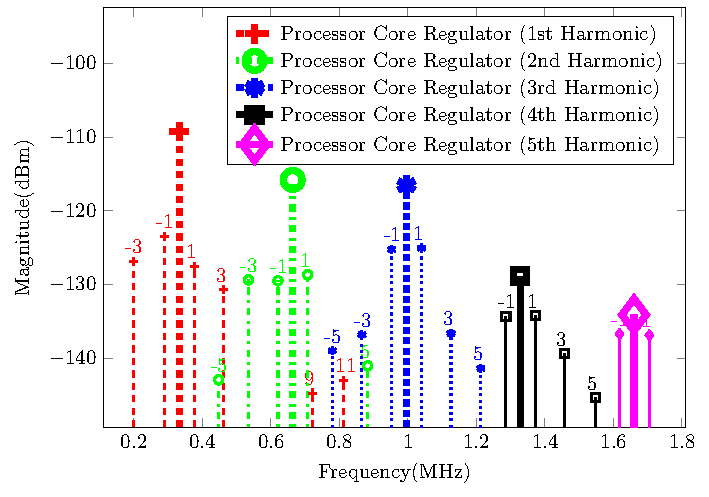
\includegraphics[width=5in]{../fase/Data/core_reg_ldl2_harm.pdf}
  \caption{Simplified spectrum representation of the harmonics of the LDL2/LDL1 activity for the Intel Core i7 desktop.}
  \label{core_reg_ldl2_harm}
\end{figure}
%\end{comment} %--------------------

The antennae we used to capture signals from computer systems were designed to detect broadcast radio signals over a wide frequency range, so they pick up these interfering signals very well. It is critical to note that FASE is intended to identify only AM signals which are modulated \textit{by our micro-benchmark}. Although AM radio signals are amplitude-modulated and strong, FASE correctly identifies that these signals are \emph{not caused by our modulation activity} and so should not be reported. This is important not only because it is painfully expensive to shield a measurement setup from broadcast signals, but also because computer systems themselves emit strong radio signals (wifi, bluetooth, NFC, etc.) that are modulated for communication purposes but should not be reported by FASE unless they are \emph{also} modulated by our microbenchmark activity.





\section{Experimental Setup}
\label{sec:fase-setup}

We evaluate the effectiveness of our FASE methodology by applying it to the laptop and desktop systems in Table~\ref{pc_specs}. Unless otherwise indicated, the EM emanations were received with a magnetic loop antenna (AOR LA400) from a distance of 30 cm and a spectrum analyzer (Agilent MXA N9020A) was used to record the spectra of the received signals. This setup was used because it allowed us to capture emanations from the entire system across a wide range of frequencies with little manual effort. We note, however, that attacks exploiting a particular set of carrier signals could likely be carried out at larger distances using more directive antennae optimized for higher gain across a narrower frequency band. 

We performed three measurement campaigns, each across a different frequency range and with different FASE parameters, as shown in Table~\ref{meas_params}. Parameters $f_{alt_1}$ and $f_\Delta$ were chosen to ensure sufficient separation between side-band and carrier, and between the peaks generated at $f_{alt_1}$, $f_{alt_2}$, etc. Aside from this consideration, the choice of $f_{alt_1}$ and $f_\Delta$ is arbitrary, with the caveat that while using only one choice of $f_{alt_1}$ and $f_\Delta$ is almost always sufficient to detect all carriers, measuring with multiple choices of $f_{alt_1}$ and $f_\Delta$ increases the confidence that all carriers have been detected. For example, a carrier might be missed if FASE is only run with one choice of $f_{alt_1}$ and $f_\Delta$ \textit{and} a carrier is weak \textit{and} strong signals happen to occur at the side-bands. We found that five alternation frequencies (i.e. $f_{alt_1}$ through $f_{alt_1}+4f_\Delta$) are sufficient to detect almost any carrier even in the presence of unrelated signals from other system activity, noise, and radio broadcasts. These experiments cover the entire AM radio spectrum, and were performed without shielding in a major metropolitan area with hundreds of radio stations nearby.

\begin{table}[htb]%
  \small%
  \centering%
    \begin{tabular}{cccc}%
    \toprule
    \textbf{Frequency Range(MHz)} & \textbf{$f_{res}$(Hz)} & \textbf{$f_{alt_1}$(kHz)} & \textbf{$f_\Delta$(kHz)} \\
    \midrule
    0 to 4 & 50 & 43.3 & 0.5 \\
    0 to 120 & 500 & 43.3 & 5.0 \\
    0 to 1200 & 500 & 1800 & 100 \\
    \bottomrule
    \end{tabular}%
  \caption{FASE measurement parameters.}%
  \label{meas_params}%
\end{table}%


The $f_{res}$ parameter is the resolution of spectrum sampling. For example, our 0-4MHz measurements used $f_{res}$ = 50Hz, so each recorded spectrum has $4\rm{MHz}/50\rm{Hz} = 80,000$ data points (frequencies). Each spectrum was measured 4 times over several hours and averaged, and we used the heuristic function in Section~\ref{sec:fase-automated} to detect the 1st, 2nd, 3rd, 4th and 5th positive and negative harmonics of the alternation activity. We then visually inspected the heuristic function's output to identify peaks (potential carriers). \cite{palshikar_2009} and \cite{alfassi_2009} present algorithms detect peaks in the output of the heuristic function, but we found that the heuristic function's output had strong spikes for carriers modulated by system activity, so the task of visually inspecting the output to identify potential carriers was relatively straightforward and quick.

A variety of activities were used as activities A and B in the alternation loop -- integer multiplication, division, addition, subtraction, as well as load and store to all levels of the cache hierarchy. The results we show focus on only three A/B alternations. The first alternates between a load from main memory (LLC miss) and a load from L1 cache (L1 hit), which we abbreviate as LDM/LDL1. This alternation is useful in exposing modulated carriers related to memory activity. We tried other A/B activity pairs that included main-memory accesses and on-chip activity, e.g. LDM/ADD, LDM/DIV, etc. and also pairings that used STM (LLC write-back activity) instead of LDM. We found that they have some variations in the exact shape and strength of the side-band signals, but applying FASE to them exposes the same carriers as LDM/LDL1.

The second A/B alternation whose results we show alternates between L2 hits and L1 hits (LDL2/LDL1). This alternation is useful in exposing carriers related to variations in activity on the processor chip. We tried numerous other pairings of on-chip activities, e.g. LDL1/ADD, LDL2/DIV, etc. and found that they expose the same carriers through FASE, although they vary in the exact shape and strength of the side-band signals.

Use of LDM, LDL2 and LDL1 is also methodologically convenient in that it uses the exact same micro-benchmark code for all three activities. They differ only in the \texttt{mask} values in Figure~\ref{fase_pseudocode}, which gives us excellent confidence that any observed modulation is due to differences between LDM, LDL1, and LDL2 activity and not the other activity (address computation, looping, etc.) in the alternation loop. Finally, note that the microbenchmarks produce a nearly 100\% load, so frequency scaling does not affect our experiments much. However, the effect of frequency scaling wasn't of interest for these measurements and so we disabled dynamic frequency scaling whenever possible.


\section{Experimental Results}
\label{sec:fase-results}
We discovered three main types of signals. First, strong signals emanate from switching voltage regulators and power filtering components at the specified switching frequency of the regulator (usually between 200 kHz and 500 kHz) or multiples of it (harmonics). These signals are modulated by variations in power consumption in the voltage regulator's load (the processor, memory or other system components), and they allow attackers to carry out the equivalent of power side-channel attacks from a distance without the need to place probes within the system. Voltage regulators for processor cores, the memory controller, and the DRAM memory itself often have different switching frequencies, giving the attacker component-by-component power consumption information. %Among voltage regulator designers, generated EM noise is a known problem and (cite saab here, explain doesn't demodulate).%we are not aware of any work that explores the implications of having the power consumption information embedded in the emanations caused by regulator switching .

Another type of signal is generated by periodic memory refreshes. This signal is amplitude-modulated by memory access activity, i.e. the attacker gets an at-a-distance readout of how often the memory is used. Unlike voltage regulators, which can be considered an external problem by processor/memory architects, these refresh-related signals are entirely caused by activity within the purview of memory controller designers and are likely to be completely eliminated by appropriate modifications to how memory refresh is carried out.

At higher frequencies, FASE discovers clock signals and their harmonics that are modulated by activity in the clock's domain. Because most clock and switching regulator harmonic frequencies are subject to electromagnetic interference (EMI) regulations~\cite{erickson_2001}, they are subjected to measures (such as spread-spectrum clocking) that spread the resulting EM emanations over a range of frequencies~\cite{hardin_1994}. In spite of this, FASE discovers such signals and provides insight into the nature of the activity that modulates them. In particular, we identify that DRAM clocks generate EM emanations which are modulated by DRAM activity. The systems tested generated weak spread-spectrum signals at CPU clock frequencies. Interestingly, we do not observe any variation in these signals in response to processor activity.

%%%%


We begin with Figure~\ref{spect_ldm}, which shows the FASE results for a recent desktop system with an Intel Core i7 processor, with the memory access modulation (LDM/LDL1) micro-benchmark. To emphasize the usefulness of FASE, we show a light gray outline of the actual recorded spectrum for one of the alternation frequencies. This spectrum is very noisy and crowded, especially in the long-wave (30-300 kHz) and AM radio (540-1600 kHz) bands, but FASE correctly indicates which signals are AM-modulated by the alternation activity. The thick vertical lines correspond to the frequency and magnitude of the modulated carrier signals automatically identified by FASE. Lines with the same color/pattern correspond to harmonics of the same frequency. A set of harmonics is likely caused by a periodic yet non-sinusoidal behavior within the system, and the magnitudes of the harmonics in a set give us important clues for identifying the source of that carrier signal. Therefore, after performing FASE it is useful to group the identified carriers into sets such that all the carriers within a set occur at frequencies which appear to be multiplies of one another.

The remainder of this section discusses how we used the information provided by FASE such as carrier frequency, harmonics, modulation depth, and modulation activity (e.g. on-chip activity or memory activity) to identify the sources of three types of carrier signals. In the systems not shown, similar types of signals were detected. 

\begin{figure}[tbh]
\centering
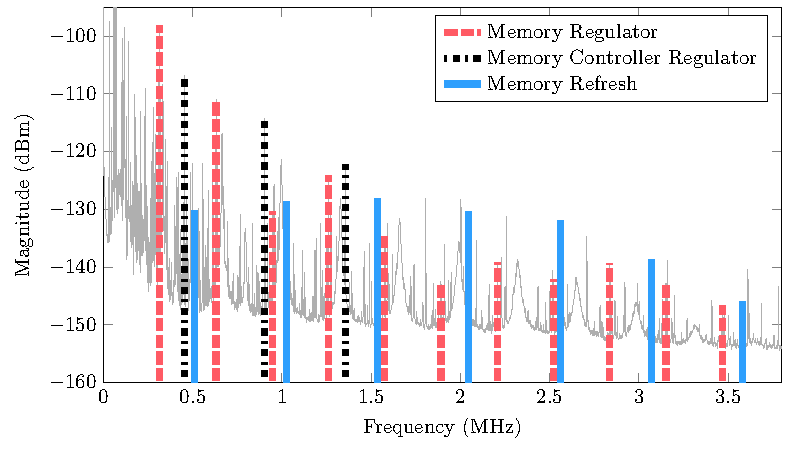
\includegraphics[trim=0.0in 0in 0in 0in,clip,width=5in]{../fase/Data/spect_ldm.pdf}%
\caption{FASE results for the Intel Core i7 desktop and main-memory (LDM/LDL1) modulating activity.}%
\label{spect_ldm}%
\end{figure}

\subsection{Switching Voltage Regulators}
\label{sec:regulators}

The set of carriers indicated by red dashed lines in Figure~\ref{spect_ldm} occurs at frequencies 315 kHz, 630 kHz, 945 kHz, etc., which are all multiples of 315 kHz. Because the even harmonics of this carrier are relatively strong we can conclude that these carriers are likely caused by some behavior that repeats at 315 kHz and has a small duty cycle. It is also helpful to look at each harmonic's shape in the spectrum. While this figure does not provide enough detail to see each harmonic's shape distinctly, the shape is very similar to that shown in Figure~\ref{core_reg_zoom} (this figure corresponds to a different regulator in the same system). The carrier's energy is spread around its central frequency by what looks like a Gaussian distribution. Clock signals for digital logic and I/O interfaces (such as memory) are tightly controlled but clocks generated by RC oscillators create carriers like the one in Figure~\ref{core_reg_zoom}.\footnote{This variation (called jitter or phase noise) is well studied because it impacts reliable communications and high frequency digital circuits~\cite{hajimiri_1998,trischitta_1989}.} 

Switching regulators often use RC oscillators. In computer systems, switching regulators convert the 12V to 24V PSU or battery voltage to 1V to 2V supplies used by processors and memory. The duty cycle of the regulator's switching signal is small when the ratio between the input and output voltage is large, which is consistent with the 315 kHz signal being related to a switching voltage regulator. We manually localized the source of the signal using an EM probe to determine where the 315 kHz EM signal was strongest in the system. We found that the signal was strongest near the high power MOSFET switches and power inductors that supply power to the main memory DIMMs. These switches were driven by a nearby switching voltage regulator IC and its switching frequency was 315 kHz, confirming our initial hypothesis. 

Once the source was found, the modulation mechanism was obvious: the regulator maintains the voltage supplied to the CPU by varying the duty cycle of the control signal of a switch between the 12V supply and the 1V output supply. For example, when DIMMs draw more current, the voltage at the regulator's output drops, so the regulator compensates by increasing the duty cycle of the switch, i.e. by connecting the 12V supply to its output for a longer fraction of the fixed 315 kHz period. When running the LDM/LDL1 microbenchmark, the DRAM regulator's duty cycle is increased during the DRAM accesses (LDM) and decreased during L1 cache hit activity (LDL1). Changing the duty cycle changes (modulates) the amplitude of all the signal's harmonics, so LDM/LDL1 activity modulates the emanated signal at the harmonics of the regulator's switching frequency.

\begin{figure*}[tb]
  \centering
    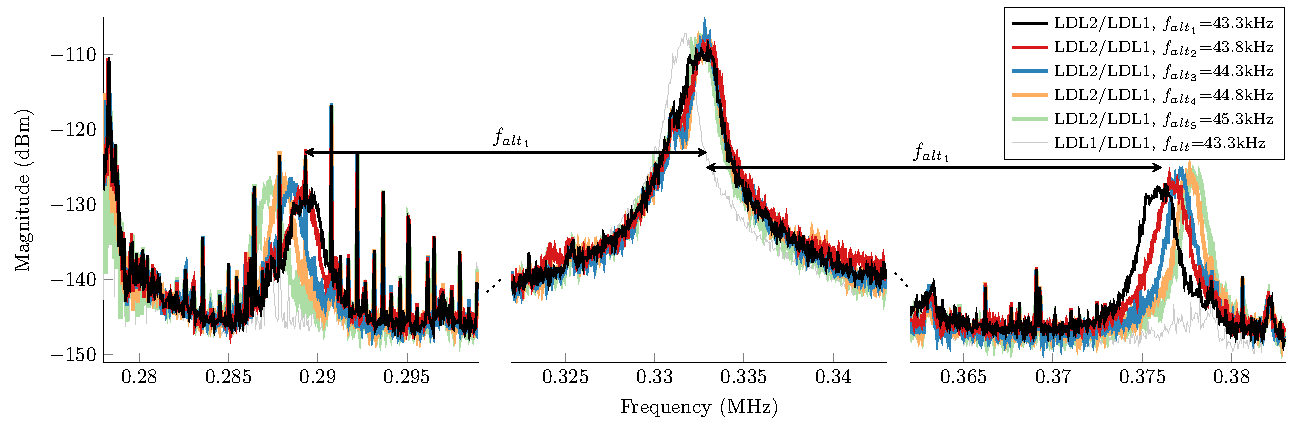
\includegraphics[width=\textwidth]{../fase/Data/core_reg_zoom.pdf}%
  \caption{A switching regulator related carrier at $f_c$ and its right and left side-bands generated by on-chip activity.}%
  \label{core_reg_zoom}%
\end{figure*}

\begin{figure}[thb]
\centering
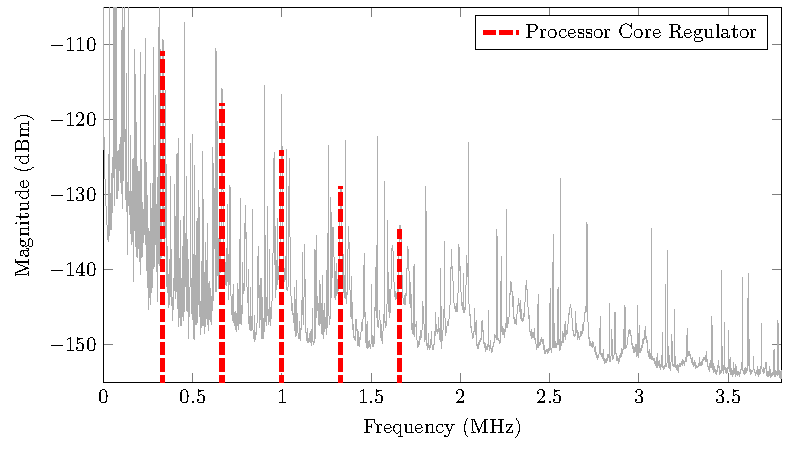
\includegraphics[trim=0.0in 0in 0in 0in,clip,width=5in]{../fase/Data/spect_ldl2.pdf}
\caption{FASE results for Intel Core i7 desktop and L2 cache (LDL2/LDL1) modulating activity.}
\label{spect_ldl2}
\end{figure}

Carrier signals indicated by black dash-dot lines in Figure~\ref{spect_ldm} are also caused by another voltage regulator. This regulator powers the on-chip memory interface (the chip has separate power supplies for its cores and its memory interface). Figure~\ref{spect_ldl2} shows the spectrum for heavy on-chip alternation activity (LDL2/LDL1). Only one type of carrier was found to be modulated in this case -- the signal that corresponds to the switching regulator for the CPU cores. Figure~\ref{core_reg_zoom} shows one of the harmonics of this signal in greater detail. We confirmed the origin of both memory interface and core regulator signals through the same near-field localization process. Interestingly, the prominent Gaussian-like shapes of the core regulator's signal are also visible in Figure~\ref{spect_ldm} but were not reported by FASE because they were not significantly modulated by the LDM/LDL1 alternation. This again illustrates that strong signals are not necessarily modulated by the activity under observation.

In many recent processors, the core CPU voltage is adjusted dynamically, while many on-chip cache and memory interface designs require fixed voltage supplies. Therefore, some processors require separate voltage regulators for the CPU and cache. As we have demonstrated, a regulator's carrier is modulated by the activity in the circuit it powers, so an attacker can distinguish cache and CPU activity by demodulating each regulator's carrier separately. Also, when separate dynamic voltage scaling is used for each CPU core, each core requires a separate regulator. When such regulator switching frequencies are not identical, attackers might be able to remotely receive a separate power consumption readout for each core, allowing attackers to remotely perform a separate power analysis attack for each core.

Finally, we note that the emerging use of in-package/on-chip regulators for processors affects regulator-related EM information leakage in new and interesting ways. On-chip linear regulators~\cite{wang_2013} do not produce modulated emanations because they have no switching frequencies to modulate. The integration of switching regulators has a more complex impact. Each integrated regulator supplies a smaller part of the chip, so the switching currents are lower and follow shorter paths, reducing emanations. However, integrated switching regulators use higher switching frequencies (e.g. 140 MHz in \cite{burton_2014}) resulting in stronger emanations. Higher switching frequencies also allow faster reactions to changes in the output voltage providing attackers with a higher bandwidth readout of power consumption.

\subsection{Memory Refresh}

The modulated carrier shown in Figure~\ref{spect_ldm} as solid blue lines has harmonics at frequencies of 512 kHz, 1024 kHz, etc. This signal did not match any previously known mechanisms that can cause EM emanations. It has a very stable frequency, indicating it was likely generated by logic that is clocked with a crystal-oscillator derived clock. Its harmonics are all of similar strength, indicating an extremely small ($<$5\%) duty cycle. Localization showed that this signal was strongest near the memory DIMMs. Additional experiments showed that the carrier signal is strongest when there is no memory activity and weakest when we generate continuous memory activity. 

This is unusual -- if this signal is caused by memory activity, we would expect it to get stronger with more activity. Further measurements with small probes close to the memory revealed many additional harmonics with a greatest common divisor of 128 kHz, not 512 kHz. This was the key clue in solving the puzzle, because 128 kHz corresponds to a period of 7.8 $\mu$s, the maximum allowable average time between refresh commands for recent DRAM standards such as DDR3.

While it would be difficult to conclusively prove that this signal is generated by memory refresh activity, the evidence strongly suggests it is. The duty cycle of the memory refresh activity is very low ($<$ 3\%) because each refresh command only lasts approximately 200 ns and occurs every 7.8 $\mu$s. The refresh timing is derived from the memory controller clock, which is crystal-derived. While DRAM standards specify that the average time between refresh commands must not exceed 7.8 $\mu$s, the memory controller has some control over the timing of the refresh commands. For example, the memory controller could postpone sending refresh commands during a 40 $\mu$s period of intense memory activity, and then ``catch up'' when memory has some idle time. This explains the strangest observation about this signal, which was that it weakens (instead of getting stronger) as memory activity increases. When the memory is inactive, the memory controller simply sends memory refresh commands at regular intervals, resulting in the strongest signal at that interval's frequency. As memory activity increases, the memory accesses increasingly interfere with the timing of the refresh commands, causing refreshes to be delayed and disrupting their periodicity (thus spreading their emanated energy across a much larger frequency range and causing the signals at 128 kHz, 256 kHz, etc. to weaken). Although the first harmonic of this signal is weaker than regulator-related signals, note that memory refresh produces many modulated harmonics and that attackers can potentially correlate them to dramatically improve their detection of this signal and its signal-to-noise ratio. It is also worth noting that since refresh timing is dictated by a standard, refresh carrier signals are present at roughly the same frequencies on all the systems we tested, which could simplify the exploitation of this leakage. This potential problem likely has an easy fix: randomizing the issue of memory refresh commands would be compatible with existing DRAM standards and would greatly reduce the modulation of refresh activity.

\subsection{DRAM Memory Clock}
%

\begin{figure}[t]
\centering
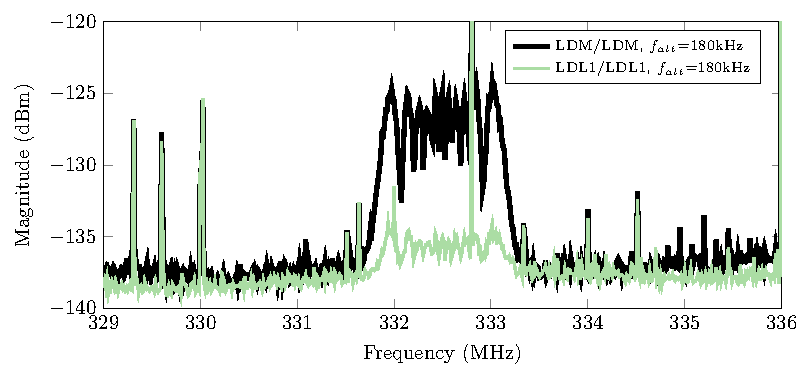
\includegraphics[trim=0.1in 0.10in 0.1in 0.09in,clip,width=5in]{../fase/Data/lx61_mem_ssc_a.pdf}
\caption{DRAM clock spectrum with 0\% (LDL1/LDL1) and 100\% (LDM/LDM) memory activity.}
\label{lx61_mem_ssc_a}
\end{figure}

\begin{figure}[b]
\centering
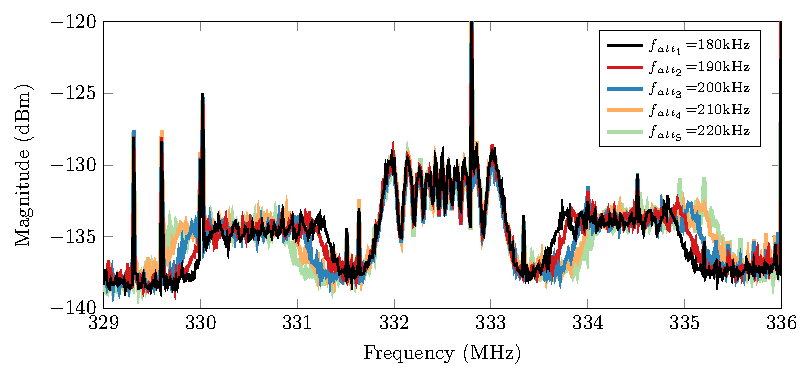
\includegraphics[trim=0.1in 0.10in 0.1in 0.09in,clip,width=5in]{../fase/Data/lx61_mem_ssc_b.pdf}%
\caption{DRAM clock spectrum with 50\% (LDM/LDL1) memory activity.}%
\label{lx61_mem_ssc_b}%
\end{figure}
Above 30 MHz, electromagnetic compatibility (EMC) standards limit the allowable level of EM emanations from consumer devices such as computers. Many periodic signals such as high frequency processor and memory clocks are strong enough to violate these limits, so alleviation techniques for these clock signals have been developed. EMC requirements specify the maximum magnitude for emissions at any particular frequency, and a popular technique (called spread spectrum clocking) varies the clock frequency periodically, spreading the emitted energy across a range of frequencies (instead of emanating it all at one frequency). For example, a 333 MHz memory clock might be swept back and forth between 332 MHz and 333 MHz over a period of 100 $\mu$s, producing a spectrum similar to %Figure~\ref{lx61_mem_ssc}\textcolor{red}{A}. 
Figure~\ref{lx61_mem_ssc_a}. While such techniques facilitate compliance, the signals are only weaker in an averaged sense: attackers can still track the carrier and use the full power of the signal after demodulation. Such ``carrier tracking'' techniques have already been developed in telecommunications to allow reception of radio signals transmitted using this technique~\cite{chung_1993}. Therefore, predictable spread-spectrum clocking does not mitigate information leakage, but it does create interesting problems for discovering such modulated carriers through manual analysis of the spectrum. The shape of the carrier and its side-bands is less recognizable, and the carrier and its side-band signals are likely to overlap significantly when using modulation activity that is not carefully chosen. 

To allow FASE to successfully detect modulated spread-spectrum clocks, it is best to set $f_{alt}$ large enough to move the side-band signals outside of the carrier's own spectrum. Figure~\ref{lx61_mem_ssc_b} shows the effect of modulating the clock signal at several such alternation frequencies.
%

\subsection{Testing the Laptop Systems}

We tested three laptop systems: one based on an Intel Core 2 Duo processor from 2010, one based on AMD Turion X2 from 2007, and one based on Intel Pentium 3M from 2002. In all three systems, FASE finds the same types of carriers we already reported: regulator-related signals, signals caused by memory refresh, and DRAM clock signals. For example, Figure~\ref{hpamd_spect_ldm} shows the modulated carrier signals found for the AMD Turion X2 system with LDM/LDL1 alternation of activity. Interestingly, the memory refresh carrier for the AMD Turion X2 laptop is at 132 kHz instead of 128 kHz as observed in all three other systems. We also confirmed a memory regulator carrier and while the two signals shown as ``unidentified'' appear to be caused by regulators, we did not confirm their sources because the laptop is very compact and taking it apart to perform localization may damage the system.

\begin{figure}[htb]
\centering
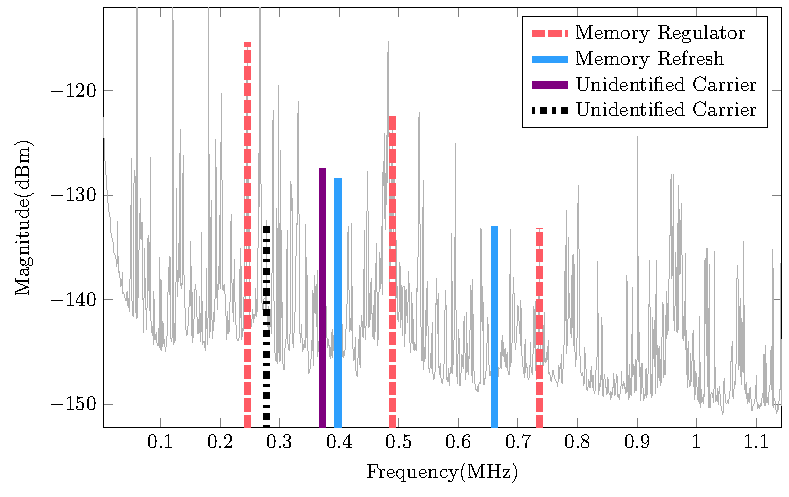
\includegraphics[trim=0.0in 0in 0in 0in,clip,width=5in]{../fase/Data/hpamd_spect_ldm.pdf}%
\caption{FASE results for the AMD Turion X2 laptop and main-memory (LDM/LDL1) modulating activity.}%
\label{hpamd_spect_ldm}
\end{figure}

The AMD system was the only system confirmed to have an activity-modulated carrier that is not reported by FASE. This carrier was emanated by the voltage regulator circuitry for the processor cores, and was \emph{frequency}-modulated (we confirmed this with a spectrogram of the modulation). Therefore FASE correctly does not report it. This particular regulator keeps the input-to-output switch turned on for a fixed amount of time during its switching cycle, but changes the duration of the switching cycle (i.e. its switching frequency) to increase/decrease its duty cycle. In principle, signals that are frequency-modulated by system activity should be possible to identify by a FASE-like approach based on spectral properties of FM-modulated signals. 

%We leave the design of such FM-seeking approaches for future work.


\section{Automating FASE}
\label{sec:fase-automated}

In Section~\ref{sec:fase-methodology}, we explained that carriers are found by searching for a shape that shifts by $f_\Delta$ when $f_{alt}$ changes by $f_\Delta$. However, visual comparison of numerous recorded spectra across a wide range of frequencies would be tedious and error prone. Equations~\ref{eq:filter_top} and ~\ref{eq:filter_detailed} a simplified and easily-implementable heuristic for finding side-bands whose shifts in frequency correspond to shifts in $f_{alt}$. For a given harmonic $h$ of $f_{alt}$, the function $F_h(f)$ is intended to have a large value for a frequency that corresponds to a activity-modulated carrier. We compute this score as 
\begin{equation}
F_h(f) = \prod_i F_{i,h}(f)
\label{eq:filter_top}
\end{equation} 
where $F_{i,h}(f)$ is a sub-score for the $i$-th recorded spectrum ($i$-th $f_{alt}$). This subscore is computed as 
\begin{equation}
F_{i,h}(f) = \frac{SP_i(f+h\cdot f_{alt_i})}{\frac{1}{N-1}\sum_{j \neq i} SP_j(f+h\cdot f_{alt_j})}.
\label{eq:filter_detailed}
\end{equation}
This function first appropriately shifts $SP_i(f)$, the spectrum captured with the microbenchmark active at alternation frequency $f_{alt_i}$, so a side-band signal at $f_c+h\cdot f_{alt_i}$ gives a peak in $F_{i,h}$ at the carrier frequency $f=f_c$, i.e. we score the side-band signals, but the sub-score is ``reported'' at $f_c$.

The value of the sub-score is computed by normalizing the strength of the side-band signal in this spectrum by the average of the other \hskip2pt $N\hskip-2pt -\hskip-2pt 1$ \hskip2pt $f_{alt_j}$ spectra. For side-band signals that do shift in frequency as $f_{alt}$ changes, the sub-score for a particular $i$ will be larger than 1 because the side-band signal is stronger at the $f_c+f_{alt}$ frequency in this spectrum. At the exact same frequency in at least some of the other spectra, however, the signal will not be as strong because these spectra have peaks at $f_{alt_j}$ and so their side-band signal is at a different frequency. In contrast, a strong signal that does not shift in frequency as $f_{alt}$ changes will stay at the same frequency in the other spectra, so the normalization will produce a score close to 1. The overall score $F_h(f)$ multiplies the sub-scores, so the overall score is close to 1 if no $f_{alt}$-induced frequency shifting occurs. If each $i$-th spectrum has side-band signals at $f_{alt_i}$, the frequency-shifted sub-scores will align producing a very large value for the carrier frequency. Finally, if only some side-band signals are present (one or a few may be ``buried'' by some unrelated signal), the overall score will be weakened because each obscured $f_{alt_i}$ side-band will have a sub-score close to 1, but the remaining sub-scores will still increase the overall score significantly above 1. Overall, this heuristic produces large peaks at frequencies of modulated carriers and is almost completely flat at all other frequencies. Figure~\ref{filter} shows the heuristic function's output for the carriers shown in Figures~\ref{mem_refresh_zoom}~and~\ref{core_reg_zoom}. Figure~\ref{lx61_mem_ssc_c} shows the heuristic function for the DRAM clock signal shown in Figure~\ref{lx61_mem_ssc_b}. FASE clearly does detect such modulated signals though it reports the clock as two separate carriers at the edges of the spread out clock signal.

\begin{figure}[htb]
  \centering
    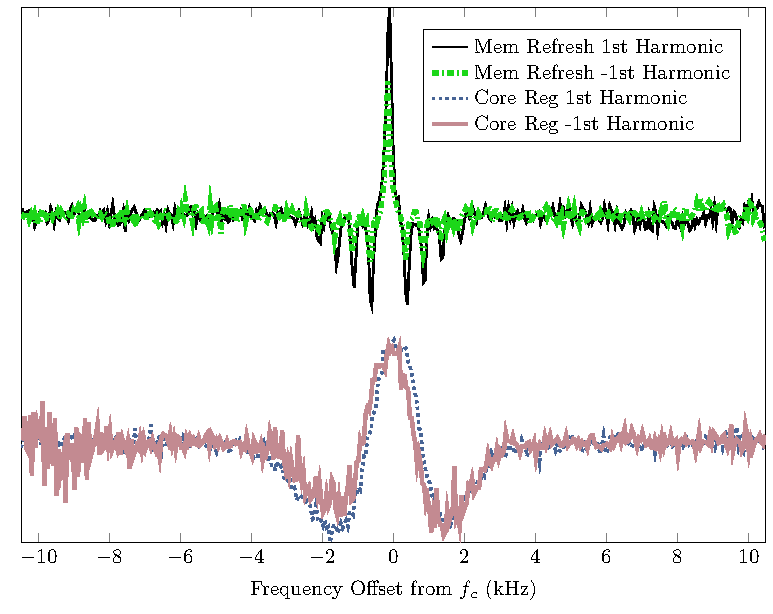
\includegraphics[width=5in]{../fase/Data/filter.pdf}%
  \caption{Output of the heuristic for the 1st and -1st harmonics of $f_{alt}$ for two carriers.}%
  \label{filter}
\end{figure}

\begin{figure}[htb]
\centering
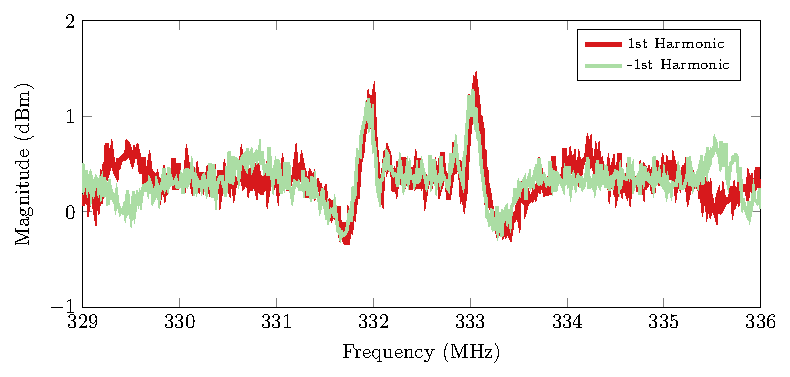
\includegraphics[trim=0.1in 0.10in 0.1in 0.09in,clip,width=5in]{../fase/Data/lx61_mem_ssc_c.pdf}%
\caption{Output of the heuristic function for an SSC DRAM clock signal.}%
\label{lx61_mem_ssc_c}
\end{figure}

The heuristic function provides a good indicator of the frequencies at which modulated carriers are likely to occur. The next step in automating FASE is to find the peaks in the $H_h(f)$ output. To do this, we sort the peaks by their prominence and keep only those with prominence greater than 1.5dB. Except for the highest peak in a spectrum, every peak sits within a valley bounded on the left and right by two higher peaks. We calculate the prominence of a peak as the magnitude of the peak in the valley minus the magnitude at the lowest point in these valley. Ideally, finding the peaks in the heuristic function would be sufficient to find all the modulated carriers. However, for realistic spectra not all peaks are caused by unintentional modulation. For example, a transient signal occurring in one of the 5 recorded spectra can cause variation in $H_h(f)$ which might be mistaken for a modulated carrier (i.e. a false positive). In such cases, the output of the heuristic alone is not sufficient to reliably report AM carriers, and some additional processing is needed.

\begin{figure}[htb]
\centering
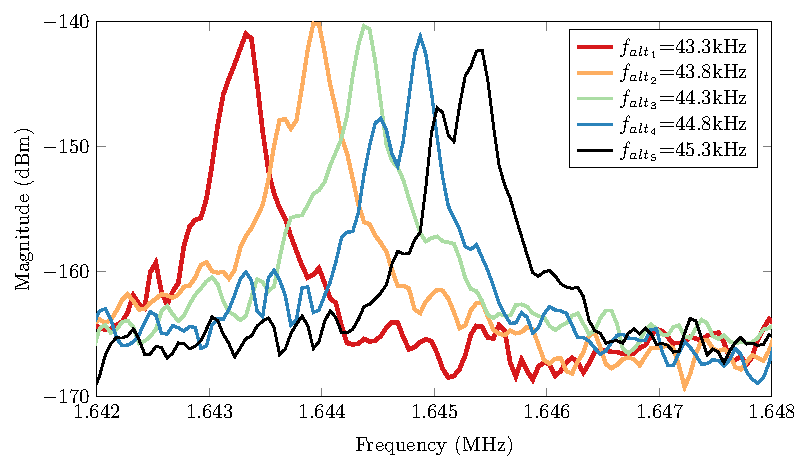
\includegraphics[width=5in]{../eucap_fase/Drawing/sb_good.pdf}
\caption{Easy to detect spectral pattern at $f_c+f_{alt_i}$ caused by an AM carrier at $f_c$=1.6MHz on the Samsung Galaxy S5 smartphone.}
\label{sb_good}
\end{figure}

Also, recall that we need to search for the spectral patterns created by FASE for 10 different harmonics ($h=-5,...-1,1,...,5$). Furthermore, the negative and positive harmonics are ``flipped.'' In other words, each peak in $H_h(f)$ is caused by a set of $N$ peaks in the spectra spaced evenly by $hf_\Delta$ as shown in Figure~\ref{sb_good}. This spectral pattern occupies a smaller or larger frequency range depending on its respective harmonic. Also, the positive harmonics (right sideband) have the $f_{alt_1}$ peak on the left and the $f_{alt_N}$ peak on the right, but the order of the peaks is reversed for the negative harmonics (left sideband). To simplify processing, when we find a peak in the heuristic function, we create a ``normalized frame.'' This normalized frame flips the signals for the negative harmonics so that the order of the peaks is the same as for the positive harmonics, and also scales the x-axis so that we have the same number of frequency points regardless of the detected harmonic $h$. After this normalization, each frame can be processed the same regardless of its harmonic. To filter out false positives, we extract relevant features from each frame and use a neural network to reduce the number of reported false positives. The extracted features and neural network are described in~\cite{wang2016}.

We evaluated the effectiveness of this automated procedure by testing it on spectra from the desktop, laptops, and smartphone systems in Table~\ref{fase_pc_specs}. The desktop and laptop measurements used a magnetic loop antenna (AOR LA400) at a distance of 30 cm as shown in on the left of Figure~\ref{sec:fase-setup}. The generally weaker smartphone EM emanations were recorded using a small loop probe with 20 turns and a 4 mm radius shown on the right of Figure~\ref{fase_auto_setup}. The smartphone probe was placed directly above the screen over the area where the induced baseband signal had the largest magnitude. The smartphone spectra were measured from 0 to 10 MHz and the computer spectra were measured from 0 to 4 MHz. We used $f_{alt_1}$ = 43.3 kHz and $f_\Delta$ = 500 Hz with five alternation frequencies (i.e. $f_{alt_1}$ through $f_{alt_1}+4f_\Delta$) and the LDM/LDL1 (DRAM memory) and LDL2/LDL1 (processor) activities. The benchmarks were run on the laptop and desktop systems as single-threaded Windows 7 32-bit user mode console applications, and were run on the smartphones as normal Android applications. When possible all unrelated programs and activities were disabled, CPU frequency scaling was disabled, and screens were turned off. The spectra were recorded using a spectrum analyzer (Agilent MXA N9020A). 

\begin{table}[htbp]%
  %\small%
  \footnotesize %
  \centering%
    \begin{tabular}{cccc}%
    \toprule
    \textbf{Type} & \textbf{Device} & \textbf{Processor} & \textbf{Carriers Found}\\
    \midrule
    %carriers found is not systematic, manual total counted
    Desktop & Dell & Intel i7 & 20 \\
    Laptop & HP & AMD Turion X2 & 7 \\
    Laptop & Lenovo & Intel Core 2 Duo & 6 \\
    Phone & Samsung Galaxy S5 & Snapdragon 801 & 7 \\
    Phone & LG P705 & Snapdragon S1 & 6 \\
    Phone & Motorola Moto G & Snapdragon 400 & 2 \\
    \bottomrule
    \end{tabular}%
  \caption{Devices for the automated FASE measurements.}%
  \label{fase_pc_specs}%
\end{table}%

\begin{figure}[htb]
\centering
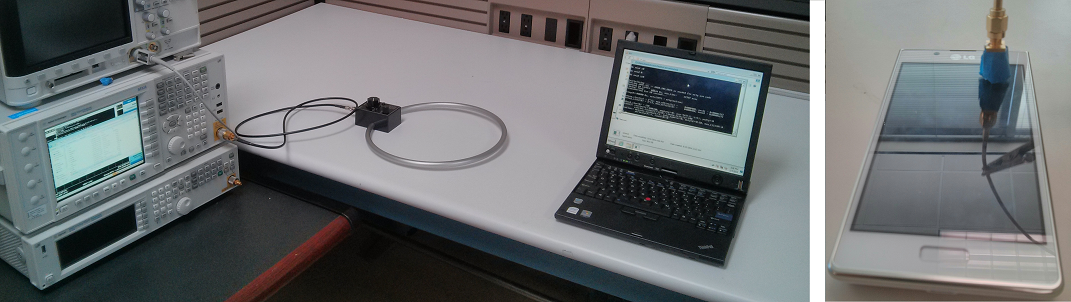
\includegraphics[width=5in]{../eucap_fase/setup.png}
\caption{Setup for the automated FASE measurements.}
\label{fase_auto_setup}
\end{figure}


%MISSED  TRUEP FALSEN FALSEP  TRUEN
%     9    129     11     21    199
%total = 149, missed =   0.06%, algo: total = 360, correct =   0.91%

We tested the six devices in Table~\ref{fase_pc_specs}, with two measurements per device (one for LDM/LDL1 and one for LDL2/LDL1). To test the accuracy of the algorithm we began by visually inspecting all the spectra and manually listing any detected signals. Determining whether a $f_{alt_i}$ spectral pattern for a given AM carrier is detectable is subjective due to the noisy and crowded nature of the spectrum. For our testing, we included only those spectral patterns where at least 3 of the 5 $f_{alt_i}$ peaks were visible. By this criteria, we found 149 spectral patterns in total by visual inspection. Nine of these patterns did not create peaks above the heuristic function's detection threshold. The heuristic functions $H_h(f)$ had 360 peaks above the prominence threshold (i.e. 360 indications of possible modulation). Frames were created for these 360 cases and tested using the neural network. The neural network predicted whether the frames corresponded to actual unintentional modulation with 91\% accuracy.

\begin{figure}[htb]
\centering
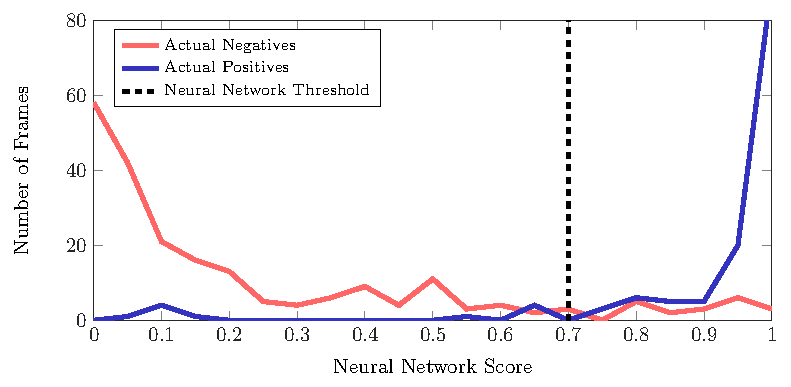
\includegraphics[width=5in]{../eucap_fase/Drawing/nn_dist.pdf}
\caption{Distribution of the neural network scores.}
\label{nn_dist}
\end{figure}

Figure~\ref{nn_dist} shows distributions of the neural network's score for the tested frames. In this figure, the blue distribution contains the 140 frames which occurred at frequencies where generated spectral patterns were caused by modulated carriers (i.e. actual positives), and the red distribution indicates the 220 frames that occurred at frequencies where no modulation was found via visual inspection (i.e. actual negatives). The dotted black line indicates the neural network threshold used. The neural network predicted all the frames to the right of this line as positive, meaning that the actual positives to the right of this line are true positives and the actual negatives to the right of this line are false positives. Similarly, false negatives and true negatives occur to the left of this line. 

Many of the true positive frames resemble the example shown in Figure~\ref{sb_good} and were easily classified as positives. Similarly, many of the true negatives were caused by random variations in the spectra and were easily classified as negatives. However, the remaining 9\% of the frames were incorrectly predicted. In some such frames, several of the $f_{alt_i}$ peaks were obscured or misshapen. For example, the frame shown in Figure~\ref{sb_hard} was correctly predicted, but had a score near the neural network threshold. As the spectral pattern's peaks became further obscured and as the shapes of the peaks became less regular, the frames were more likely to be incorrectly predicted (i.e. false negatives). Similarly, false positives occurred where random variations in the spectra create patterns that resemble the spectral patterns generated by AM modulation.

\begin{figure}[htb]
\centering
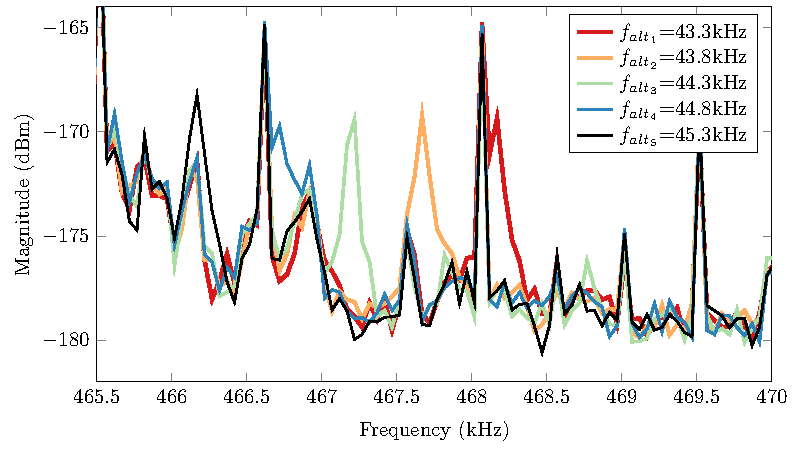
\includegraphics[width=5in]{../eucap_fase/Drawing/sb_hard.pdf}
\caption{Difficult to detect frame at $f_c-f_{alt_i}$ for an AM carrier at $f_c$=511kHz on the Lenovo laptop.}
\label{sb_hard}
\end{figure}

% samsung s5 circuit descriptions: 
% http://www.techinsights.com/teardown.com/samsung-galaxy-S5-teardown/
% this is where the battery connects to the phone, so I'm assuming voltage regulator
%https://www.ifixit.com/Guide/LG+Optimus+L7+P705+Charger+Port+Replacement/33461

The unintentional AM carriers found for the desktops and laptops were caused by voltage regulators, memory clocks, and memory refresh commands. For the smartphones, several carriers were found to be caused by voltage regulators. The remainder of the carriers found on the smartphones could be traced to particular IC packages or modules and were determined to be modulated only by memory activities. However, smartphones integrate many system components into System on Chip (SoC) modules and often use Package on Package (PoP) technology to integrate both the processor and memory into the same package and little information is publicly available describing these components. More information would be needed to definitively determine the circuits and mechanisms modulating these carriers.



\section{Summary}
Efficient targeted mitigation of side-channel vulnerabilities requires finding information-leaking signals and determining how information is embedded into these signals. In this chapter we described FASE, a novel methodology for automatically finding which EM-emanated signals from a computer system are amplitude-modulated by specific program activities. FASE uses the SAVAT microbenchmarks to generate detectable spectral patterns in the side-bands of all the carrier signals that are AM-modulated by specific system activities, automatically processes measured spectra to identify these patterns, and calculates the frequencies of the modulated carriers.

This approach has several advantages. First, it directly identifies the carrier frequencies modulated \textit{by specific system activities}, which goes a long way toward determining the sources of compromising emanations. Second, it is robust against the interference of unmodulated signals and noise inside and outside of the system, such as AM-modulated signals and carrier-like signals which are not specifically modulated by system activity. Third, it quantifies how strongly carrier signals are modulated, which is useful for identifying how the carrier is generated, for quantifying information leakage, and for evaluating the effectiveness of mitigation efforts. Fourth, it is specifically designed to robustly detect unintentionally modulated signals, which have several inconvenient features not found in ideal AM signals. Finally, each FASE evaluation requires only a few spectrum measurements while other techniques such as DPA require thousands of spectrum captures with different keys and plaintexts~\cite{sugawara2009}. 

To demonstrate FASE's effectiveness, we applied it to several computer systems and found activity-modulated signals generated by voltage regulators, memory refresh activity, and DRAM clocks. Our results indicate that separate signals may carry different information about system activity, potentially enhancing an attacker's capability to extract sensitive information. We also confirm that our methodology correctly separates emanated signals that are affected by specific processor and/or memory activity from those that are not.

We also presented an algorithm for automatically measuring FASE. We demonstrated the algorithm's performance on several different types of processors and systems (desktops, laptops, and smartphones) and compared the results to an exhaustive manual search. We also verify that all signals identified by the algorithm can be traced to plausible unintentional modulation mechanisms to illustrate that these signals can potentially cause information leakage. 

FASE can be used to find which parts of a system leak information about some aspect of program activity. Once the source of the leak is found, the strength of modulated signals can be reduced and the modulation can be weakened, i.e. we can disrupt the connection between program behavior and the variations in activity that modulate such signals. Using memory refresh signals as an example, this would involve randomization of the interval between refresh commands, while modulation-weakening efforts might involve careful scheduling of memory accesses to avoid their interaction with refresh activity.




\chapter{ZOP: Zero-Overhead Profiling via EM Emanations}
\label{zop}
\label{sec:zop}

\section{Overview}
Program profiling is a type of dynamic analysis that measures some aspects of software behavior. One of the most common instances of program profiling counts the execution of instructions or sequences of instructions and uses that information to identify heavily executed paths (also called \textit{hot paths}). Knowledge of the hot paths can guide other tasks such as code optimization and performance analysis. Profiling is typically implemented by adding software probes (instrumentation) to a program's source code or binary executable and these probes either log events of interest or update statistics about such events at runtime.

%after deployed, don't want to change code
This approach is effective in many usage scenarios, but there are a few exceptions. Adding instrumentation unavoidably adds runtime and resource overheads. Runtime overheads can alter the timing of events, and so in real-time systems or cyber-physical systems these timing changes can affect the path taken through the profiled program.  In fact, if overheads are high enough, these systems may fail (\eg miss real-time deadlines) if they are profiled under ``in the field'' conditions. Profiling is also challenging in already deployed software~\cite{kraft2010}, where a deployed system that suffers performance problems would ideally be profiled \textit{in situ} to ensure that the profiling results capture the actual program behavior in that deployment. Although hardware features can reduce the software overhead required for detailed profiling, they can rarely eliminate it completely. Moreover, these solutions are costly in terms of chip/PCB space and development time, and feature support varies between devices.  Profiling embedded controllers presents additional challenges, as these devices often lack sufficient memory space to store the extra code (instrumentation) and profiling-related data structures. They also sometimes lack the I/O interfaces to report the profiling results back to the programmer.

An ideal profiling solution would be one that gathers (1) perfectly accurate information about what is actually executed during profiling (2) without changing anything about the profiled system: no code instrumentation, no data structures for profiling information, no additional I/O activity, and no changes to the hardware of the system. While instrumentation can provide perfectly accurate profiling information, it is an inherently intrusive technique that---even when minimal and designed so as not to affect the semantics of the instrumented code---changes some important aspects of the code's dynamic behavior.

These properties make program profiling an attractive target application for software analysis via EM emanations. This chapter proposes \zop\ (Zero-Overhead Profiling), a technique that retains the second aspect of ideal profiling (no changes to the profiled code or system) at the cost of less-than-perfect accuracy. \zop\ computes profiling information in a highly accurate and completely non-intrusive way by leveraging electromagnetic (EM) emanations generated by a system as the system executes code. Because \zop\ generates profiling information without interacting with or modifying the profiled system, it offers the potential to profile a variety of software systems for which profiling was previously not possible. In addition, the ability to collect profiles by simply placing a profiling device next to the system to be profiled can provide advantages over traditional instrumentation-based approaches in many traditional contexts as well.

\zop\ first measures the EM emanations produced by the system to be profiled as the system processes inputs whose execution path is known (\textit{training} phase). This allows \zop\ to build a model of the waveforms produced by different code fragments. \zop\ then collects emanations from a new, unknown execution and infers which parts of the code are being executed at which times (\textit{profiling} phase). This inference is accomplished by matching the observed unknown emanations to emanations from the training phase that are known to be generated by particular code fragments.

This chapter presents:
\begin{itemize}
\item \zop, a completely non-invasive profiling approach, where profile information is inferred from EM emanations of the (unmodified) system as it runs the (unmodified) to-be-profiled software.
\item A proof-of-concept implementation of \zop\ that shows that our approach is practically feasible.
\item Experimental results that (1) show that \zop\ can achieve high profiling accuracy and (2) provide insight into the performance of \zop\ that suggest directions for further research.
\end{itemize}

In the rest of the chapter, Section~\ref{zop-background} describes at a high level how program execution can be related to EM emanations, Section~\ref{sec:approach} describes how \zop\ generates a training model and uses EM emanations along with this training model to generate profiling data for new program executions, and Section~\ref{sec:evaluation} describes an implementation and experimental evaluation of \zop.


\section{Relating Time Domain EM Emanations to Program Behavior}
\label{zop-background}


As demonstrated by the work done for SAVAT and FASE, computing devices generate electromagnetic (EM) emanations when they operate. While previous research has demonstrated that useful information about a system's behavior may be embedded in these emanations (\eg \cite{Rao02a,genkin_2014,CALLAN2014}), it also suggested that such information extraction on devices with highly optimized microarchitecture can be difficult in practice. Nearly all existing techniques for extracting information from EM emanations are used for side channel analysis in cryptography, and are thus focused on extracting information about {\em a specific value used by the program}, such as a cryptographic key.  Furthermore, these techniques operate in an adversarial context; that is, they must overcome program and hardware features (countermeasures) that are specifically designed to mask or obfuscate the impact that the desired data values have on EM emanations.

Profilers have a few advantages over side-channel attackers. First, the profiled system is cooperative, so there are no countermeasures in place, and the profiler may position probes wherever needed to get the best EM signal. Also, program profilers record statistics about when and how often parts of a program execute and are not primarily focused on data values. Sequences of instructions and control flow decisions affect EM emanations more strongly than changes in data values, potentially making profiling information easier to extract than data values.

While the details of how computing devices generate EM emanations are complex, a brief example describing the EM emanations produced by a processor's clock may provide some helpful insight into the connection between EM emanations and program behavior. At each cycle of a processor clock, the processor state is updated, generating a current at the clock's frequency.  Conceptually, the amplitude of this current depends on how much of the processor state changes at each cycle; that is, the current depends on which instructions are active or have been recently executed.  As a program executes, the processor executes different instructions based on control flow decisions, and this variation in instruction execution modulates the amplitude of the processor clock current. EM emanations from the processor can be directly related to the current drawn by the processor. These phenomena together create a direct link between the processor clock EM emanations and program behavior. \zop\ uses this link to determine which code executes and how frequently.

% Alex: the next paragraph is a bit confusing.
If a program executes several times with the same inputs, the waveforms of the EM emanations recorded during program execution may vary significantly between program runs. EM noise from other devices, radio broadcasts, or communication signals can cause these run-to-run variations. However by demodulating the signal at the frequency of the processor clock, one can filter out any noise outside of the narrow band of the RF spectrum around that clock frequency. Furthermore, specially designed EM probes and signal processing can be used to filter out noise with properties distinguishable from our signal of interest (\eg eliminate noise and signals not generated by the processor). In addition to external noise, system activity unrelated to the program and the accumulation of small timing differences caused by the complexity of the system (\eg cache and memory behavior) can also create run-to-run variations between repeated executions with the same inputs. However, these variations are usually smaller than the waveform differences created by execution of different paths through the program. Therefore, by observing a sufficient number of dynamic instances of the same static path, it is possible to later recognize this path by matching it against one of its dynamic instances. For example, if a short path has two dynamic instances, one with a cache miss and one with a cache hit, it is possible to recognize this path as long as there are examples of both possible dynamic instances. We will explain in Section~\ref{sec:profiling} how the ability to recognize short paths can be used to predict complete paths through a program.

\begin{figure}[htb]
  \center
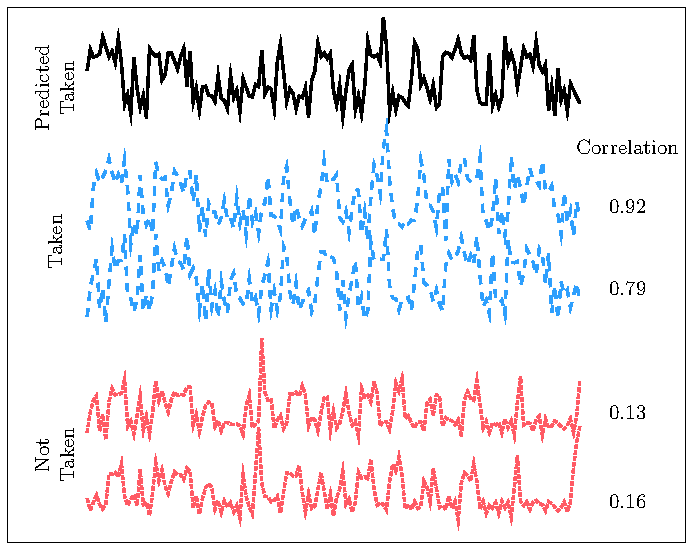
\includegraphics[width=5in]{../issta_profile/profiling/figures/branch_predict}
\caption{Examples of waveforms collected by measuring EM emanations produced by several executions.}
\label{fig:branch_predict}
\end{figure}

Figure~\ref{fig:branch_predict} shows several waveforms recorded during a short fragment of program execution. All of these waveforms start at the same static location in the program, and each follows one of two paths depending on whether the $true$ or the $false$ path of a conditional statement is followed. In particular, the dashed waveforms correspond to execution along the $true$ (conditional branch instruction is ``taken'') path, whereas the two dotted waveforms correspond to execution along the $false$ path (branch instruction is ``not taken''). Assume we use dynamic analysis to determine whether the branch is taken for these cases. It is clear from Figure~\ref{fig:branch_predict} that while there are some differences between these ``training'' waveforms that correspond to the same path, these differences are smaller than those between the $true$ and $false$ paths. To determine which path was taken in the ``unknown'' (solid) waveform without doing any dynamic analysis, we calculate the correlation coefficient between that unknown waveform and each of the candidate recorded waveforms. By observing correlation coefficients, we are able to determine with high confidence that the branch was taken in the unknown execution, as the branch-taken examples correlate much better with it than the branch-not-taken examples.

% reviewer 3: Compare ZOP to a “dumb” approach that just guesses based on likelihood
% \alex{General question: How would our result compare to an approach
%   that uses symbolic analysis for this? Did anybody try that?}


\section{The ZOP Approach }
\label{sec:approach}
In this section, we (1) introduce the \zop\ approach, (2) describe how we can create a model that encodes training waveform features and (3) use this model to predict the path taken during an unknown execution using only the waveform produced by this execution without using \textit{any} runtime instrumentation.


The goal of \zop\ is to compute code profiling information without any instrumentation. Figure~\ref{fig:overviewzosp} shows a high-level overview of our approach. As the figure shows, \zop\ has two main phases. In the \textit{training phase}, \zop\ runs instrumented and uninstrumented versions of the program against a set of training inputs, records EM emanations for these executions, and builds a model that associates the recorded waveforms with the code subpaths that generated them.  In the \textit{profiling phase}, \zop\ records the EM waveform generated by an execution of a vanilla (\ie completely uninstrumented) version of the program, finds the closest match between sections of this waveform and the waveforms in the training model, and uses the matching subpaths to predict the overall path taken by the execution being profiled. \zop\ implements these two high-level phases in the steps and substeps shown in the workflow portrayed in Figure~\ref{fig:system_diagram}. In the next sections, we explain the different steps and substeps in this workflow in detail.

\subsection{Training 1}
\label{sec:training-1}

The left part of Figure~\ref{fig:system_diagram} shows the Training~1 phase of the \zop\ approach.  During Training~1, \zop\ runs an instrumented version of the system against a set of training inputs.  This step is needed to reconstruct a graph model of the program's states, to determine the timing of each subpath, and to establish the correspondence between subpaths and the EM waveforms they generate.  We refer to the instrumentation points as \hbox{``markers''} since they are used to ``mark'' the time of each executed instrumentation point in the EM waveform. In order to ensure optimal placement of these markers for generating accurate profiling information, the level of granularity of the inserted instrumentation points (markers) is critical.

\begin{figure}[tb]
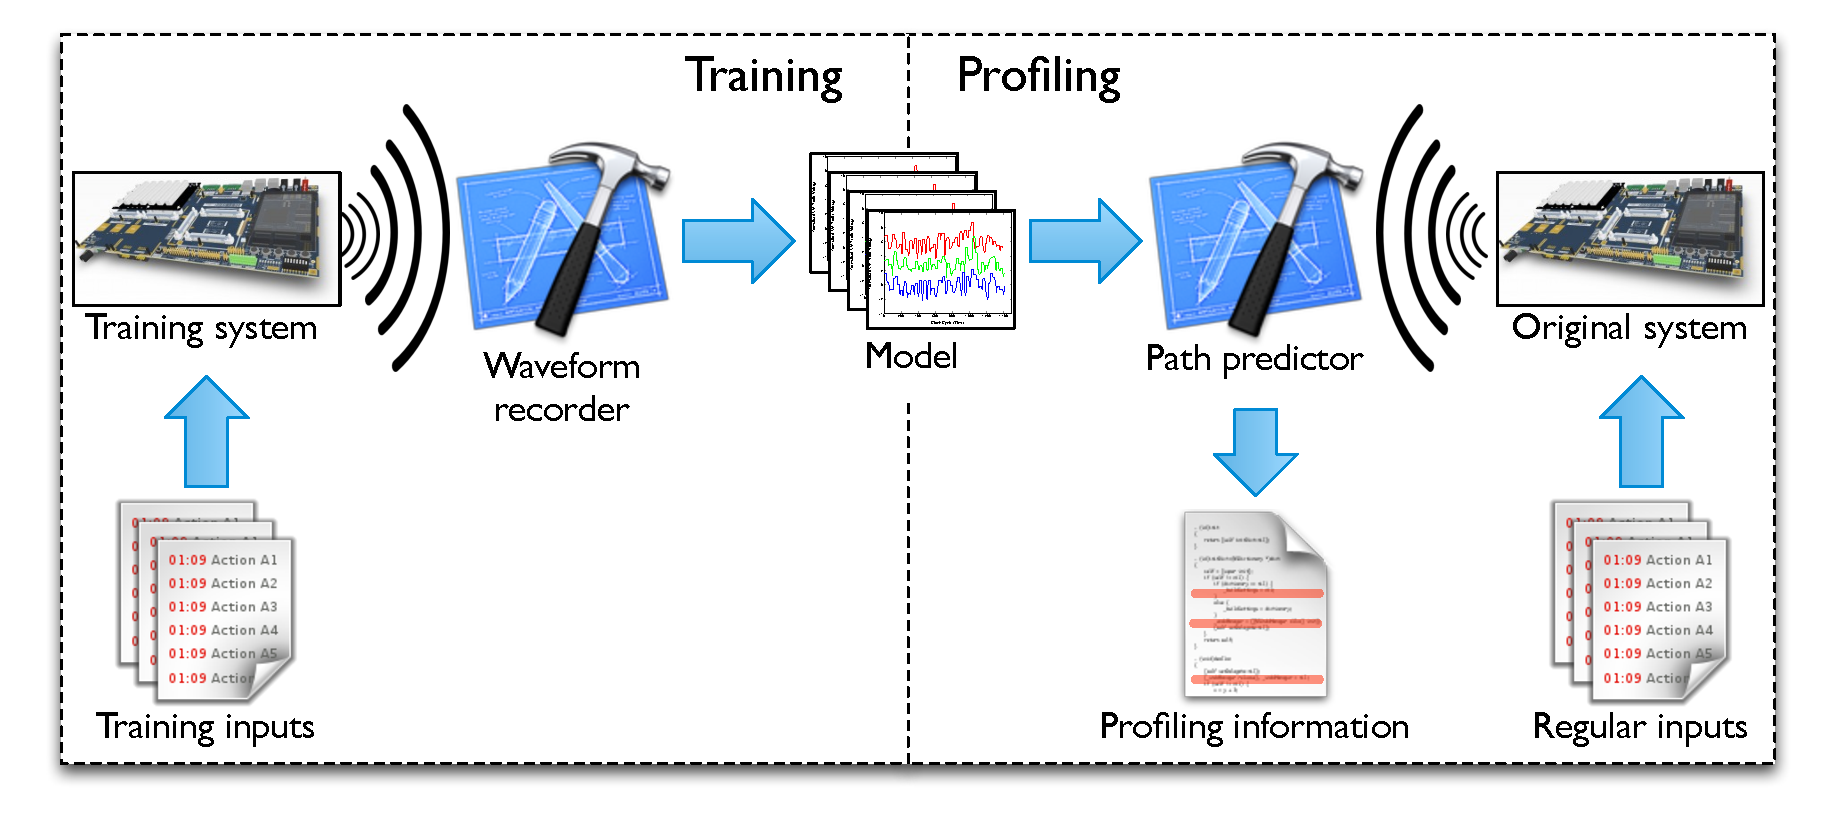
\includegraphics[width=5in]{../issta_profile/profiling/figures/overviewzosp}
% \vspace{-8pt}
\caption{High-level view of our approach.}
\label{fig:overviewzosp}
\end{figure}

\begin{figure*}[tb]
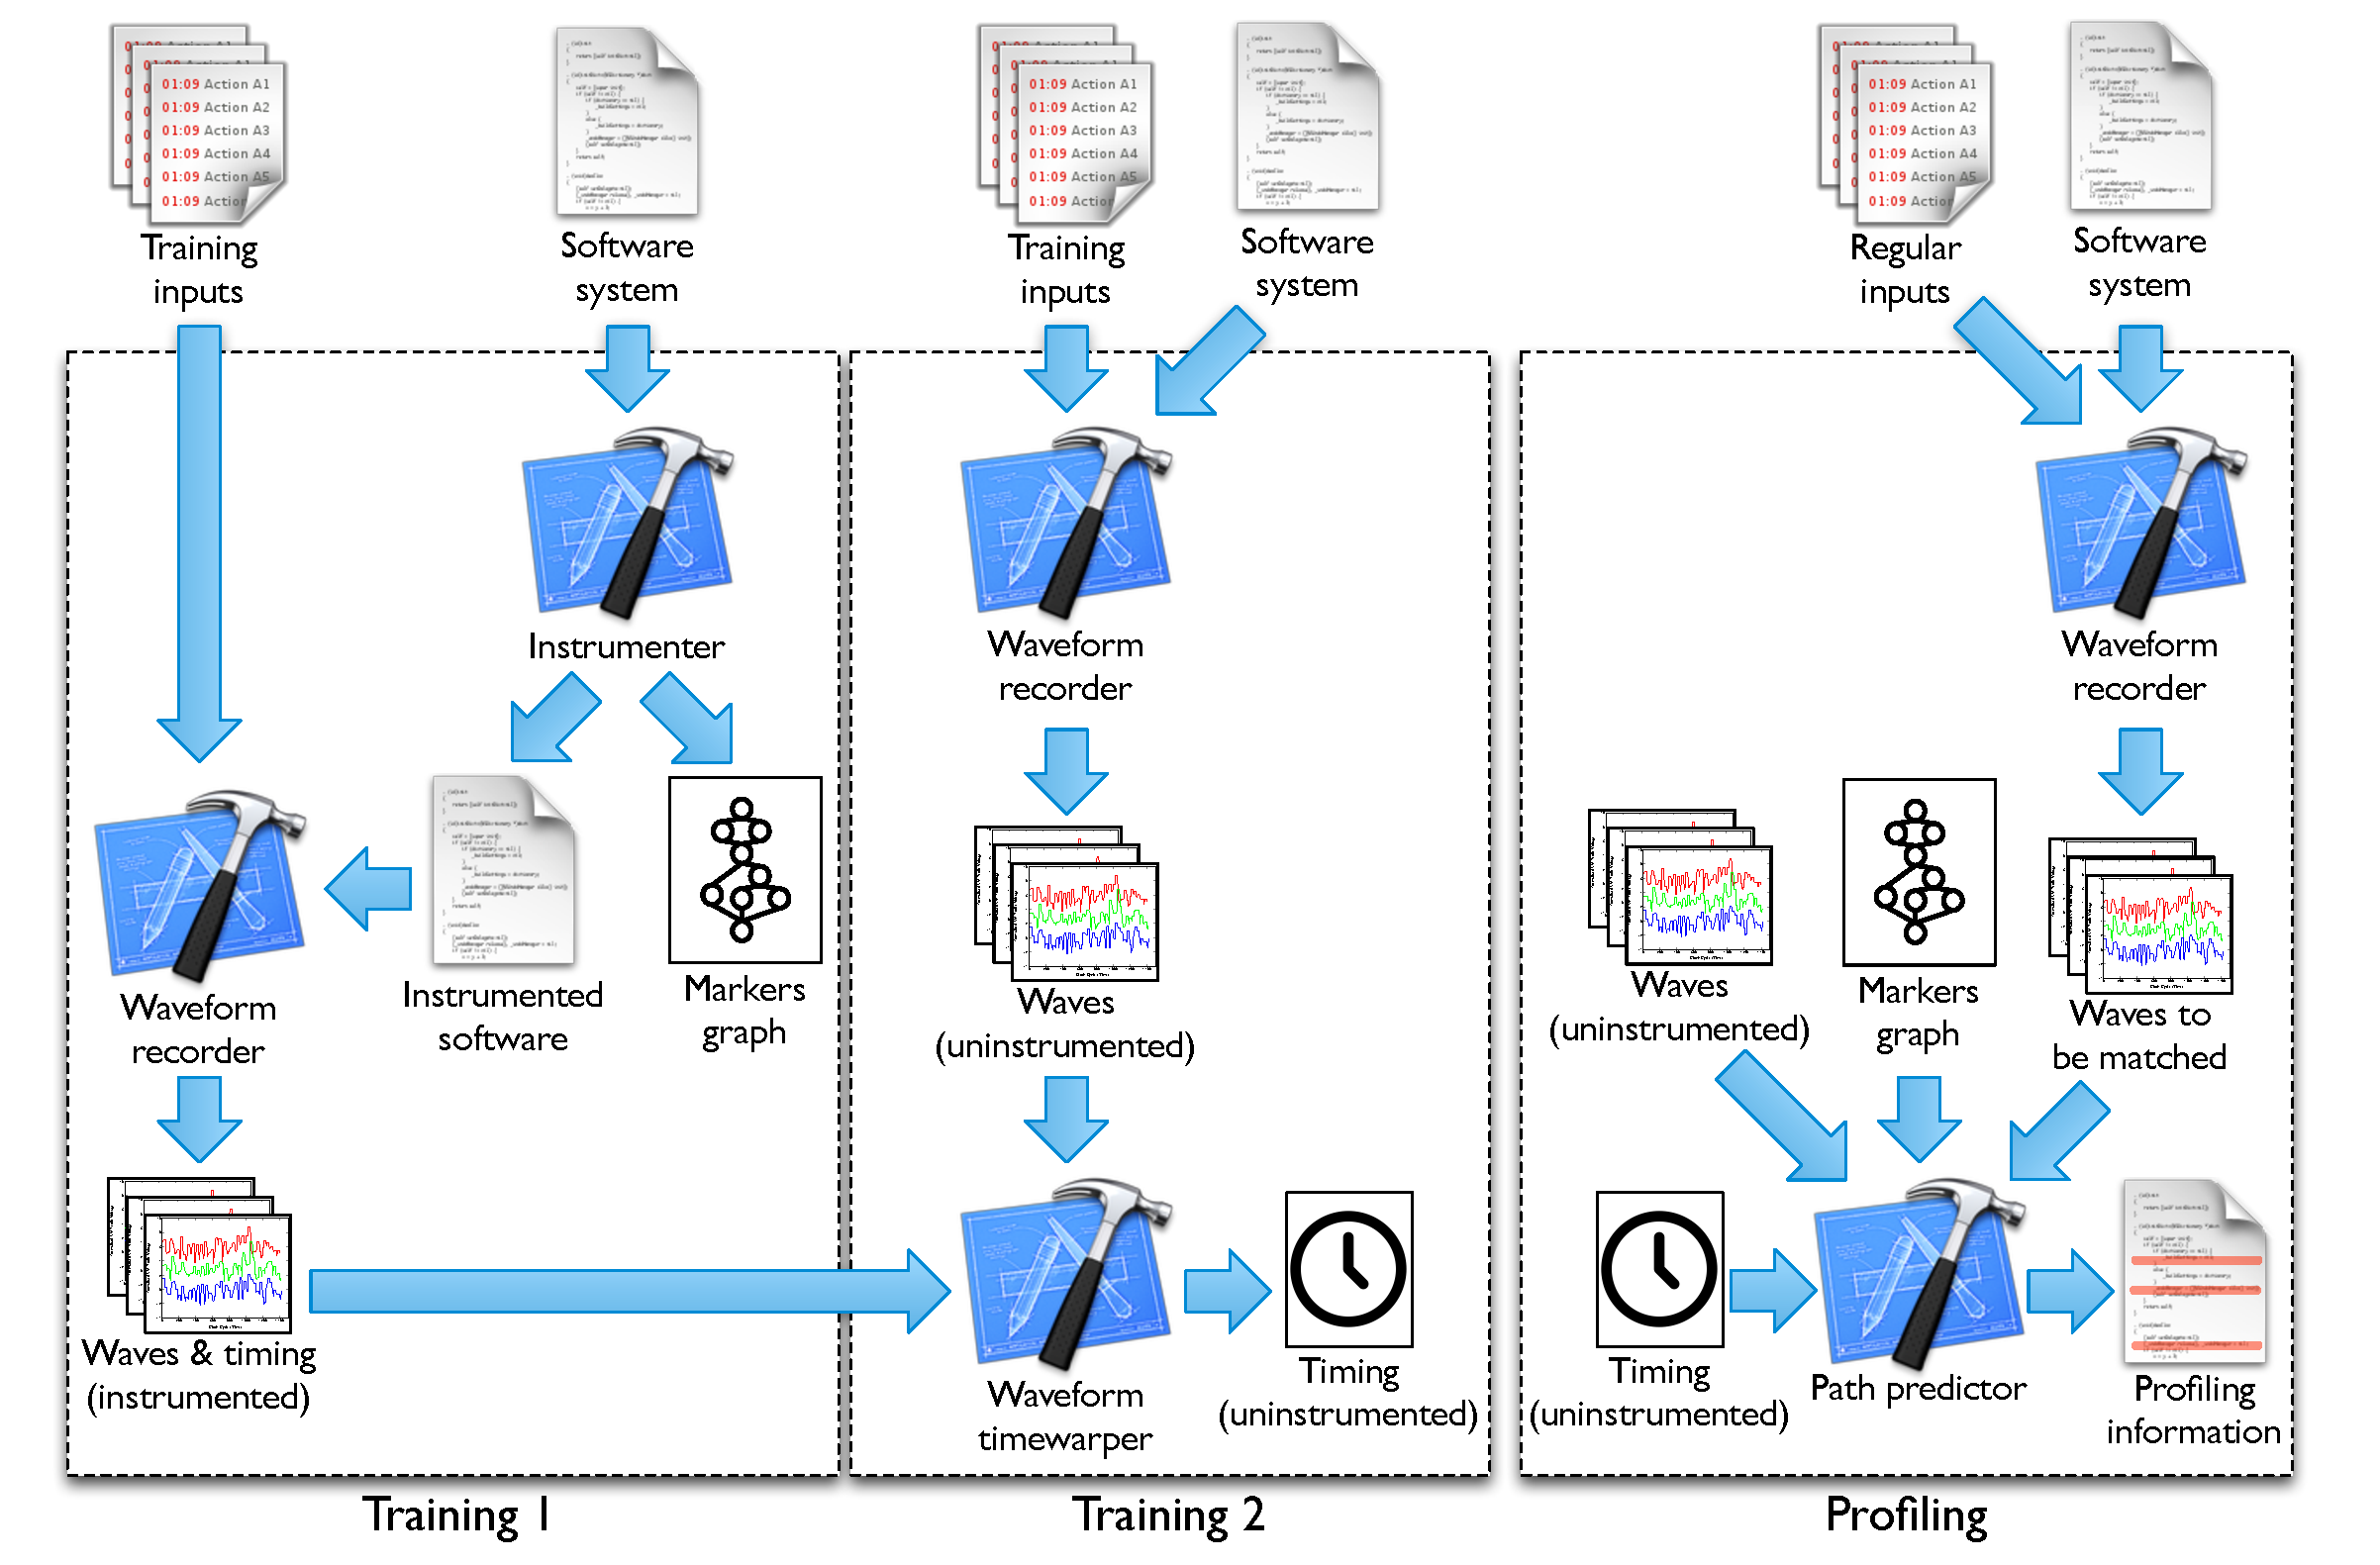
\includegraphics[width=\textwidth]{../issta_profile/profiling/figures/workflowzosp}
\caption{Workflow of \zop. (Note that we repeat some elements to reduce clutter, improve clarity, and better separate the different  steps of the approach; that is, multiple elements with the same namerepresent the same entity.)}
\label{fig:system_diagram}
\end{figure*}

% SPACE \subsubsection{Operating at the Right Level of Granularity}
%9)Reviewer1:In 3.3.1, ``statements'' should be ``instructions''/''basic blocks''.
In general, matching the EM emanations waveform from an unknown execution path to example waveforms for known execution paths is not a simple task. Matching complete program executions is clearly not an option, as it would require observing all possible executions to build a model. An ideal model would, in fact, be one that learns the waveform for each processor instruction independently, as this would make path recognition easiest. Some recent research matches waveforms on an instruction by instruction basis~\cite{scandalee,msgna2014} for non-profiling applications, but this technique has only been applied to the simplest of processors and has not yet been successfully applied to path profiling.

Based on our experience and preliminary investigation, we contend that longer subpaths must be considered for this matching to be successful in more complex processors, where superscalar out-of-order microarchitecture and variable latency memory interfaces make instruction by instruction recognition impractical. Therefore, in our approach, we consider acyclic paths, as defined by Ball and Larus~\cite{Ball:1996:EPP:243846.243857}, as the basic profiling unit. (Intuitively, acyclic paths are subpaths within a procedure such that every complete path in the procedure can be expressed as a sequence of acyclic paths.)  In other words, \zop\ learns the waveforms generated by the execution of acyclic paths exercised by the training inputs and then tries to recognize these paths based on their waveforms during profiling. The acyclic paths provide a level of the granularity that simultaneously (1) keeps the marker to marker paths short enough that a reasonable number of training examples can represent all the possible marker to marker waveform behaviors and (2) keeps the training instrumentation overhead low enough that the instrumentation itself does not drastically affect the execution waveforms.

% SPACE \subsubsection{Instrumenter}
The \textbf{\textit{Instrumenter}} module starts by computing the acyclic paths in the code~\cite{Ball:1996:EPP:243846.243857}.  For every identified path in the source code, it adds markers in the source code to identify such paths. (Typically, the markers are placed at the beginning and end of each path.) The instrumentation locations are similar in spirit to those of lightweight program tracing approaches, such as~\cite{ohmann2013}.

The example code shown in Figure~\ref{fig:example_code} consists of a C function called \texttt{putsub}, which is a slightly simplified version of a function present in one of the programs we used in our evaluation (see Section~\ref{sec:evaluation}).  Marker positions for this example function are shown in Figure~\ref{fig:segment_match_code}.  Each time a \texttt{marker()} is encountered, the marker ID (\eg A,B,C, etc.)  and the time elapsed since the start of the program are recorded in an array.  To illustrate with an example, consider an execution of \texttt{putsub()} that takes the path ABDEF. The recorded values would show the time when A was encountered, followed by the time when B was encountered, and so on. For each training input, \zop\ runs the instrumented code and records the EM waveform. It then ``marks'' the EM waveform with the current program location each time a marker is encountered. With this information \zop\ could find, for instance, all the start and end times for the instances of the AB subpath in the training executions and extract the portions of the EM waveforms for these times. It is important to stress that instrumentation is only used during the Training~1 phase, and the program profiled during the Profiling phase is unmodified and uninstrumented. It is also worth noting that, while the location of the instrumentation points for \texttt{putsub()} results in a unique basic block subpath between each pair of instrumentation points, this is not a requirement for our approach.

\begin{figure}[tbh]
\begin{small}
\lstset{language=C++,basicstyle=\ttfamily\small,numbers=left}\lstset{escapeinside={/*@}{@*/}}
\begin{lstlisting}[frame=none,xleftmargin=30pt]
void putsub(char* lin, int s1, int s2, char* sub) {
  int i = 0;
  while (sub[i] != ENDSTR) {
   if (sub[i] == DITTO) {
     int j = s1;
     while (j < s2)
       fputc(lin[j++], stdout);
   } else	
     fputc(sub[i], stdout);
   i++;
  }
}
\end{lstlisting}
\caption{Uninstrumented \texttt{putsub()} function.}
\label{fig:example_code}
\end{small}
\end{figure}



\begin{figure}[t]
\begin{small}
\lstset{language=C++,basicstyle=\ttfamily\small,numbers=left}\lstset{escapeinside={/*@}{@*/}}
\begin{lstlisting}[frame=none,xleftmargin=30pt]
void putsub(char* lin, int s1, int s2, char* sub) {
  int i = 0;
  marker(A);
  while (sub[i] != ENDSTR) {
   marker(B);
   if (sub[i] == DITTO) {
     int j = s1;
     while (j < s2) {
       marker(C);
       fputc(lin[j++], stdout);
     }
   } else	{
     marker(D);
     fputc(sub[i], stdout);
   }
   i++;
   marker(E);
  }
  marker(F);
}
\end{lstlisting}
\caption{Instrumented \texttt{putsub()} function.}
\label{fig:segment_match_code}
\end{small}
\end{figure}

% SPACE \subsubsection{Markers Graph}
The \textbf{\textit{Markers Graph}} models the possible paths between marker code locations. As an example, Figure~\ref{fig:mark_graph} shows a graph derived from the \texttt{putsub()} function in Figure~\ref{fig:segment_match_code}. The graph's nodes are the markers for \texttt{putsub()}, and a directed edge occurs from marker X to marker Y if the program can reach Y from X without reaching another marker in between. While this graph shows a single edge between X and Y, there may be thousands of training examples for each such two marker subpath. Therefore, to predict the whole execution path, we need to not only predict the next marker but also the time the execution took to get from X to Y.
%Furthermore, there may be multiple basic block sequences that lead from X to Y.

\begin{figure}[tbh]
\centering
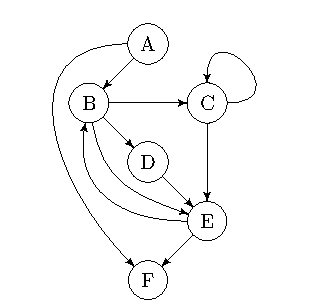
\includegraphics[width=4in]{../issta_profile/profiling/figures/mark_graph}
\caption{Marker graph for the \texttt{putsub()} example.}
\label{fig:mark_graph}
\end{figure}

%SPACE \subsubsection{Waveforms and Timing}
%\label{sec:record_waves}

The \textbf{\textit{Waveforms and Timing}} block of Training~1 contains the recorded waveform examples for subpaths in the program for which the correspondence between an execution's waveform and the code path taken is known. These waveforms, however, are affected by the computations done by the instrumentation, so they will not directly match uninstrumented code during profiling. \zop's next step is thus to collect waveforms for the same training inputs, this time without instrumentation, and identify the times in these instrumentation-free waveforms that correspond to marker positions in the code (even though the uninstrumented code has no markers at these positions).

\subsection{Training 2}
\label{sec:train2}

The middle part of Figure~\ref{fig:system_diagram} shows the Training 2 phase of the \zop\ approach.  In this phase we run an uninstrumented version of the code with the same set of inputs used in Training~1, collect the waveforms for these executions, and perform matching to determine the points in these new waveforms that correspond to marker positions in the corresponding waveforms from Training~1. This results in waveforms generated by uninstrumented execution, but in which we do not know which part of the waveform corresponds to which marker-to-marker part of the program code. These waveforms must be compared to those observed during profiling to infer which part of the code is executing at each point in the profiling run. To do this, we must infer the timing of the uninstrumented code, \ie we must determine which part of the instrumentation-free (Training~2) signal corresponds to which part of the instrumentation-marked (Training~1) signal and thus, transitively, to determine which portions of the waveforms collected during profiling correspond to which subpaths in the instrumentation-free program code.

% how different can training 2 and profiling be from training 1?
%9)Reviewer1:Training and profiling require the same compiler,
%optimization, and general processor architecture, but not the exact
%same processor/system.  
%1)Reviewer1:How can you train systems where instrumentation is
%unacceptable? Training1 can take place in a different SW/HW
%environment than Training2 and profiling (e.g., on development HW
%with more resources). This is the key advantage of using two training
%phases (Fig.4).
This two-phase training approach has the key property that, while the device/environment used for Training~2 must be similar to that used for Profiling, the device/environment used for Training~1 can differ from that used for Training~2 and Profiling. For example, \zop\ could perform Training~1 on a development board with more resources and flexibility, to facilitate the required instrumentation, and then perform Training~2 and Profiling on a production system that does not have the resources or flexibility to handle instrumentation (since neither of these phases requires instrumentation). Training~2 could then be done on a production system by software developers, whereas Profiling could be done directly on a deployed system, while real users interact with it. 

\subsubsection{Inferring Timing for the Uninstrumented Code Using Time Warping}

%Recall that the features and time spent in each subpath is a function
%of processor and memory activity and unfortunately the instrumentation
%at the marker points is no exception. 
The key to identifying which uninstrumented (Training~2) waveform corresponds to which part of the code is that, for each training input, we have executed the code twice, once with the instrumented program and once with the uninstrumented program. This means that the path through the code is the same for both executions, and that the EM signals for the two executions will tend to be similar at points that correspond to execution between markers, but one of the signals (the one from Training~1) has additional (marker instrumentation) activity inserted, along with some distortion of the signal at the transitions between instrumentation and ``real'' program activity. An example matching between instrumented and uninstrumented execution waveforms for the same training inputs is shown in Figure~\ref{fig:time_warp}.  The longer red waveform (at the top of the figure) corresponds to an execution of the instrumented code, and the vertical solid black lines show the (known) timing of the markers as recorded by instrumentation. The shorter waveform (at the bottom of the figure) corresponds to an uninstrumented execution, where timing of the markers is not known because the code is not instrumented. Note that the instrumented and uninstrumented waveforms share many of the same features, but there are also significant differences (see, for instance, the DE and BC paths). These differences are often larger than the differences between two unique dynamic instances of the same subpath, so profiling accuracy would be poor if \zop\ simply used (instrumented) waveforms from Training~1 to match to signals collected during (uninstrumented) profiling.

%Furthermore, it is not feasible to calculate the timing for an uninstrumented execution directly from the timing of an instrumented execution of the same inputs. This is primarily because the amount of time spent in the \texttt{marker()} function depends on the context of the code used to create a marker. Small random differences in the timing might be expected to cancel out but some systematic differences do exist. For example a marker in one \texttt{for} loop may take slightly less time on average than a marker in a different \texttt{for} loop. These differences result in a large timing drifts if the \texttt{for} loops have many iterations. Hence, a more reliable method is needed to infer timing in the uninstrumented code. 

To systematically determine which part of the Training~1 signal corresponds to which part of the Training~2 signal for the same input, a technique such as dynamic time warping~\cite{senin2008} can be used. In general, time warping between two signals can cut out parts of the top signal (shifting later samples of this signal to fill the gap made by the cut-out) in such a way that the remaining samples of the top signal are as similar as possible to the bottom signal. After time warping, \zop\ knows which points in the instrumentation-free waveform correspond to the marker points in the instrumented-run waveform, as shown by the dotted lines in Figure~\ref{fig:time_warp}.

\begin{figure}[t]
\centering
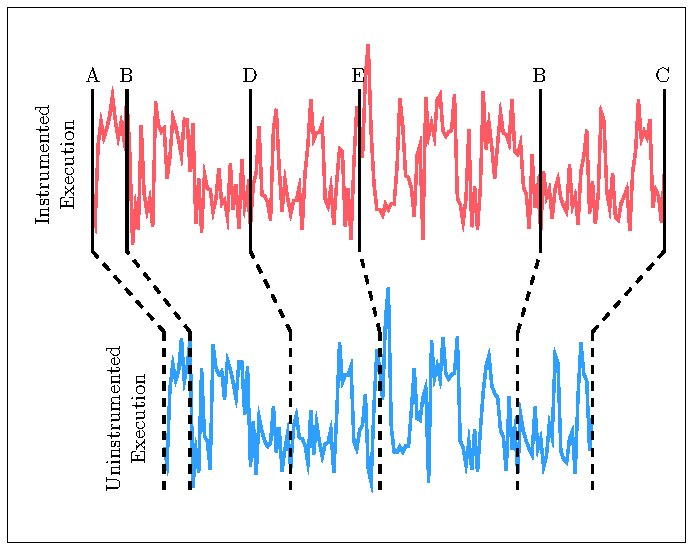
\includegraphics[width=5in]{../issta_profile/profiling/figures/time_warp}
\caption{Estimating path timing in uninstrumented training executions using waveform time warping.}
\label{fig:time_warp}
\end{figure}

\subsection{Profiling}
\label{sec:profiling}

The right column of Figure~\ref{fig:system_diagram} shows the Profiling phase of \zop. In the Profiling phase, we run the uninstrumented program with the to-be-profiled inputs, record the EM waveforms produced, and compare these waveforms to the waveforms collected (and annotated with marker information) in Training~2.

\begin{figure*}[t]
\centering
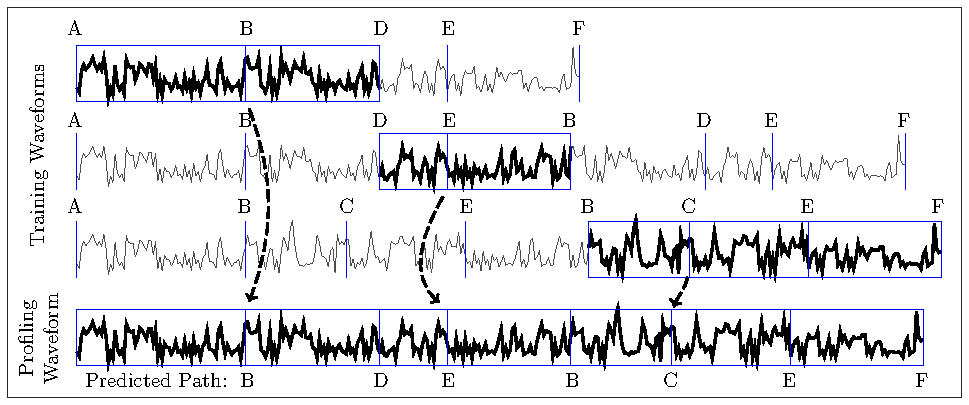
\includegraphics[width=\textwidth]{../issta_profile/profiling/figures/segment_match}
% SPACE \caption{Predicting the execution path of the \texttt{putsub()} example by matching waveform segments of three training executions to a execution waveform.}
\caption{Predicting an execution path through \texttt{putsub()} by matching training waveform segments to an execution waveform.}
\label{fig:segment_match}
\end{figure*}


\subsubsection{Path Predictor}
\label{sec:path_predict_algo}

The Training~1 and 2 phases of \zop\ yield waveforms and marker timing information for the set of training inputs used in the uninstrumented program as well as the markers graph. When a particular short subpath occurs during the profiling program execution, the resulting waveform will be similar to a training waveform of that same short subpath. To predict, for example, the execution path taken by the \texttt{putsub()} function, we run the uninstrumented version of \texttt{putsub()} with a to-be-profiled input and record the waveform shown at the bottom of Figure~\ref{fig:segment_match}.

To illustrate how our \textit{Path Predictor} works, here is one example. For the profiling waveform shown in Figure~\ref{fig:segment_match}, we start with no information about the path taken. According to the markers graph, the profiling execution must start with marker A at the beginning of the waveform. The next marker encountered can be either B or F according to the marker graph. We use the Pearson correlation coefficient~\cite{wherry1984} to compare the profiling waveform with the three training waveforms in Figure~\ref{fig:segment_match}. All three training waveforms start with an AB subpath which very closely matches the start of the profiling waveform. Although it is not shown, assume that we have another training example with the AF path and this AF waveform does not match the profiling waveform. Then we can infer that the profiling execution starts with the AB path and that B occurs at the same time in the execution as it does in the training executions. There are two possible next subpaths from B, either BD or BC. Examining all the training waveform sections for BD and BC, it is clear that the profiling waveform matches the BD section in the top training waveform more closely than it does the BC section in the third training waveform. Therefore we can infer that the profiling execution takes the BD path. From D the only possible next marker is E, so we find the most closely matching DE waveform and update our predicted path to ABDE. From E the code encounters either F or B next. Comparing the EF and EB waveforms, it is clear the profiling execution has taken the EB path next. We repeat this waveform matching and path updating process until we reach the exit marker F. This process predicts the ABDEBCEF path.

Figure~\ref{fig:segment_match} and its description captures the essence of the training and path prediction algorithm but some refinements are needed to achieve adequate performance. Consider what happens when an incorrect prediction is made. For example, assume we incorrectly selected ABCE at the start of the profiling waveform instead of the correct path ABDE. In such a case not only is the subpath through C wrongly predicted but in addition even though we have predicted D correctly as the next marker, the time of the D marker is too early. When we match the training subpaths starting at D assuming this incorrect time for D, the training waveforms may no longer match the profiling waveform well. Blindly selecting the most closely matching next subpath is not guaranteed to result in the most closely matching waveforms for the entire execution. Such errors tend to compound and the predicted execution path may diverge from the actual execution path indefinitely. This issue may be even worse when an incorrect marker is predicted and the predicted path and the actual path diverge for a long time following the incorrect decision. To address these issues we need to model the search for the optimal execution path more precisely.

\subsubsection{Path Prediction as a Tree Search}
When we reach a marker X at a particular time $t$ in the profiling waveform we compare all the training subpath waveforms starting at X against the profiling waveform starting at $t$ and assign a score to each training example. We use the correlation coefficient as the similarity metric between the section of the profiling waveform starting at $t$ and the training subpath waveform. Therefore for each training example we get a correlation value, a next marker, and the time of the next marker (\ie the start time $t$ plus the duration of the training subpath).

We can think of the search for the optimal execution path through the program as a tree search. The root node is the entry marker (marker A in Figure~\ref{fig:segment_match_code}) and each child node has an edge for each training subpath example starting at that node's marker. Each node in this tree has a marker (\eg A, B, C, etc.) and a starting time $t$ in the profiling waveform. Each edge corresponds to a single training subpath example waveform and has three properties: a duration (the duration of the training example), a correlation between the training subpath waveform and the profiling waveform starting at time $t$, and the marker at the end of the subpath in this training example. According to these definitions a search tree for an example execution waveform of \texttt{putsub()} can be made as shown in Figure~\ref{fig:backtracking}. Each edge in the figure denotes a training example subpath and its waveform. The edge weights shown are the correlation values for each edge's training example (only the highest correlated subpath edges are shown).

\begin{figure}[t]
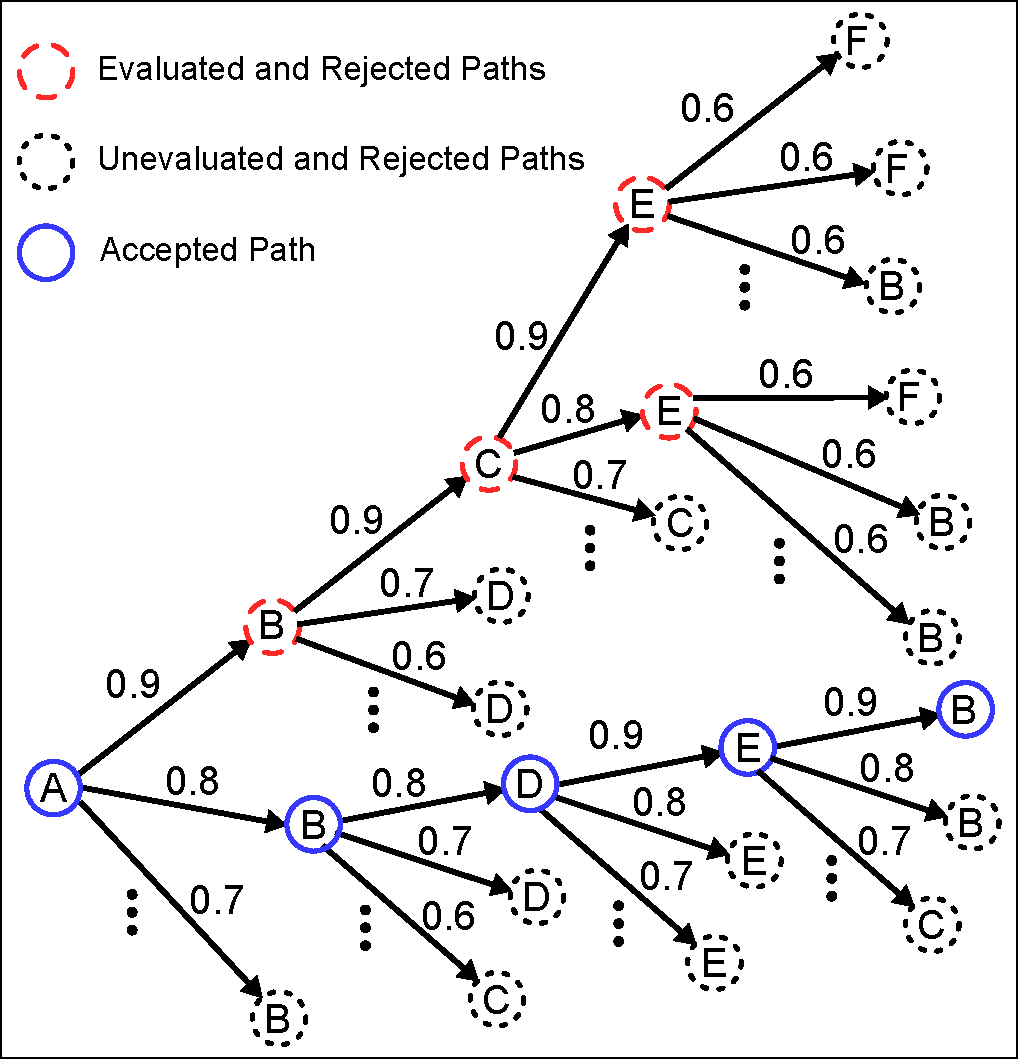
\includegraphics[width=4in]{../issta_profile/profiling/figures/backtracking}
\caption{Example of path prediction through tree search.}
\label{fig:backtracking}
\end{figure}

The branching factor for these trees is large because each node may have thousands of training examples. To simplify the search, we employ the following heuristic. The goal of the heuristic is to find a root-to-leaf path whose edges all have correlation greater than a chosen value $C_{th}$. To evaluate a node, we calculate the correlation of each next edge and sort the nodes in order of decreasing correlation. If the edge with the maximum correlation is greater than $C_{th}$ we continue searching along this edge. Otherwise, we indicate this node as rejected and backtrack along our path so far (\ie toward the root node). As we backtrack we stop at the first node that has an edge to an unevaluated node with correlation greater than $C_{th}$ and search forward along this edge.  In Figure~\ref{fig:backtracking}, $C_{th} = 0.75$, and the search algorithm follows the red dashed nodes from A to B to C to E along the top-most edges. No edge from this E node exceeds $C_{th}$, so the algorithm backtracks to C and then continues forward to the E node with $C_{th} = 0.8$. Again, no edge from here exceeds $C_{th}$, so the algorithm backtracks along C to B to A and moves forward along the accepted blue path.
%4)Reviewer1:What if the path beyond the next marker differs for
%training and profiling signals?  
Because \zop\ identifies paths by matching short subpaths between marker pairs and backtracks when unsuccessful, it can recognize paths that it never observed during training.

This heuristic clearly results in a path where each edge is greater than $C_{th}$, if such a path exists, since \zop\ only follows edges with correlation greater than $C_{th}$. However, it is not guaranteed that all paths that meet our selection criteria correspond to the correct whole program execution path. It is also not guaranteed that a path meeting the selection criteria exists.
%9)Other clarifications for Reviewer1: -We will add references to and
%compare against existing tree-search algorithms. Investigating
%alternative matching algorithms is a possible future research topic.
It is worth noting that many sophisticated heuristic algorithms exist for searching through trees with similar properties~\cite{browne2012,ruml2002,korf1985,biglieri1991}, so we believe that future research in this area can greatly improve the overall path prediction accuracy.
% Our results show this simple algorithm works adequately in practice,
% assuming the refinements mentioned below are implemented.

Two minor refinements are required to make this algorithm practical. First, when correlating the training examples against the profiling waveform it is necessary to correlate the waveforms several times with slight misalignments between the training waveforms and the profiling waveforms and use the best result of all the alignments. This is because the current position in the program is always an estimate, so by trying several different alignments and selecting the best alignment, \zop\ can keep track of the current program location with better accuracy. The second refinement is that the training waveforms for each edge are extended beyond the time position of the next marker so that all the training waveforms starting at a given marker have the same length. This is done by finding the training example for each marker with the longest duration and extending the other training example waveforms for this marker to the same length. This is required to allow fair comparisons between training examples which would otherwise have different lengths (shorter signals are more likely to be more highly correlated due to random chance than longer signals). This approach has the added benefit that (with some preprocessing) all the training waveforms for a given starting marker can be correlated (with several different alignments) against a profiling waveform using a single matrix multiplication which greatly reduces runtime.

%SPACE\subsubsection{Eliminating Redundant or Impossible Search Paths}
\subsubsection{Pruning Search Paths}
Removing nodes before they are evaluated can greatly decrease runtime because the evaluation of each node in this tree is expensive and the tree branches quickly. Some nodes can be rejected quickly without sacrificing much accuracy. For example, suppose two edges W and Z start at a node B and represent BD training waveforms with nearly identical durations. This repetition is common because executions of the same subpath often have roughly the same runtime. Suppose W has higher correlation to the profiling waveform than Z. We can immediately reject Z without evaluating it because the D node following W and the D node following Z occur at the same time in the profiling waveform (since W and Z start at the same time and have the same duration). If W is evaluated and rejected, evaluating Z would just re-evaluate an identical D node with nearly the same start time.

We can eliminate more edges by observing that many marker sequences do not correspond to valid execution paths. To see this, recall that the path prediction execution paths are interprocedural and that we allow an edge from any marker X to a marker Y if an X to Y transition is possible in the profiling program. Then consider a function which contains a single marker F. This function is called from two points A and B in the program, returning at points C and D respectively. Then the only valid marker sequences for this function call would be AFC and BFD. The algorithm described so far would however also evaluate the impossible paths AFD and BFC. Ideally, a fully constrained grammar of all possible paths would be generated to limit the search to possible marker sequences. This grammar could enumerate the set of valid next markers from any node in the search tree. This grammar would be difficult to generate, so instead we keep a function call stack for the currently evaluated execution path and any next marker which would be inconsistent with the call stack is rejected. Note this is a very weak constraint and only eliminates the impossible AFC and BFD sequences when A and B are in different functions.

% there are many more topics that can be described here:
% marker at start and end of function, placement of markers not needed for
%\rob{Rob needs to add description of marker placement, standard library calls, alignment of segments, fixed correlation length, variability of a given path, time between markers varies}

\subsection{Profiling Information}
\label{sec:predict_path}

In the final step of \zop, we construct the paths for the profiling inputs from a set of predicted markers provided by the previous steps. Every consecutive pair of predicted markers represents a set of basic blocks that are executed between two markers by a training input. First, for every training input and every two consecutive pair of markers we extract the basic blocks that are executed between them.  Once \zop\ collects the basic blocks between each pair of markers, it uses this information to generate the predicted whole program basic block path from the sequence of predicted markers. The profiled acyclic paths can be easily identified and counted from this whole program path.

\subsection{Usage Scenarios}

Describing the usage scenarios where \zop\ presents an attractive alternative to existing solutions, we must first be more specific about the requirements for using \zop. First, and most obviously \zop\ requires hardware for demodulation, waveform recording, and signal processing. It is expected these requirements can be met by existing software defined radio receivers. Second, \zop\ also inherits most of the requirements of existing profilers such as instrumentation insertion. Third, \zop\ requires a set of inputs to be used for training. These training inputs must have a coverage of the short subpaths in the program most similar to branch coverage. In most scenarios where an application is to be extensive profiled such a set of inputs exists. The next and final requirement is more subtle. During training the program is instrumented and run to record waveforms and timing information. This raises the question ``If it is possible to run the program with instrumentation, why go through all the trouble of recording and processing waveforms just to count the executed paths?''

There are several reasons for this. First, in many applications it may be feasible to run a program with several short inputs that provide good branch coverage in a testing environment but may not be feasible to instrument the system in a production environment or in the field. This is likely the case for code with realtime requirements or operating system code. In other cases it may be possible to record the profiling information but there may be no easy way to get the profiling information off the device. Second, \zop\ is unique in that it can provide profiling information with no hardware support or direct interaction with the system while it is being profiled. Some computing systems have hardware support for profiling (performance counters, instruction traces, etc.) but these methods require hardware support (both logic on-chip and in some cases large connectors on the PCB) and do affect some system properties such as power consumption. Third, we believe the approach used by \zop\ will find applications beyond profiling such as malware detection and debugging where functioning without instrumentation is desirable for other reasons.


\section{Experimental Results}
\label{sec:evaluation}
To assess the usefulness and effectiveness of our approach, we developed a prototype tool that implements \zop\ and performed an empirical evaluation on several software benchmarks. (For simplicity, in this section we use the name \zop\ to refer to both the approach and its implementation, unless otherwise stated.) In our evaluation, we quantified (1) the accuracy of the profiling information computed by \zop and (2) how the training inputs used affect \zop's accuracy. In the rest of this section, we discuss our implementation of \zop, our evaluation setup, and the results of our evaluation.

% The first research question assesses how the \zop\ profiling results
% compare to profiling results from existing profiling techniques. The
% second research question explores the impact that the number of
% training examples of a path has on the profiling accuracy for that
% path.

\subsection{ZOP Implementation} 
\label{sec:implementation-1}

For our evaluation, we used a NIOS II processor on an Altera Cyclone II FPGA. This processor has many of the features of modern complex computer systems (\eg a 32 bit RISC MIPS-like architecture, a large external DRAM, separate instruction and data caches, dynamic branch prediction) while also providing features that were extremely useful for developing our understanding of how program execution affects the system's EM emanations (\eg programmable digital I/O pins, access to programmable logic, and cycle-accurate program tracing). For the evaluation, we did not use any FPGA-specific features.

We leveraged LLVM~\cite{LLVM} to detect the acyclic paths in the code, identify instrumentation points, and insert instrumentation. We then used LLVM's C backend to generate instrumented C source code. GCC then compiled this source code to a NIOS binary. Both the original and instrumented source code are standard C code and could be compiled and run on any modern architecture.

The software parts of \zop are built using freely available software (\ie compiler, code analysis framework, and FPGA tools). To observe EM emanations, we used a magnetic field probe (a small inductor in series with a tuning capacitor) that was placed directly over the processor's decoupling capacitors. The EM probe was assembled by hand by one of the authors from components that can be bought for less than \$10. Finally, we used a spectrum analyzer (which can be a fairly expensive piece of equipment) to demodulate and record EM emanations so as to have more control and flexibility in our investigation, but numerous software defined radio receivers, which are available for less than \$1,000 have sufficient capability and precision to reproduce our measurements.

\subsection{Evaluation Setup}
\label{sec:evaluation-setup}
\begin{table}[htb]
  \begin{center}
    \caption{Statistics for the SIR benchmark profiled by ZOP.}
    \begin{tabular}{|c|c|c|c|c|}
      \hline
      Benchmark & LOC & Markers
      & Training Set Size
      & Profiling Set Size \\
%      & \multicolumn{1}{m{0.4in}|}{\centering Path \\ Profiling \\ Accuracy}  \\
      \hline
      \hline
      print\_tokens & 571 & 48 & 240 & 400 \\
      \hline
      schedule      & 415 & 36 & 284 & 400 \\
      \hline
      replace       & 563 & 54 & 299 & 400 \\
      \hline
      Total        & 1549 &138 & 823 & 1200 \\
      \hline
    \end{tabular}
    \label{table:benchmarks}
  \end{center}
\end{table}

We selected three programs in the SIR repository~\cite{Software-artifact} to profile: replace, print\_tokens, and schedule. Table~\ref{table:benchmarks} shows, for each benchmark, its name, its size, the number of markers added during training, and the number of inputs we used during the training and profiling phases.

%5)Reviewer1/Reviewer2:How would ZOP scale to more/larger programs?
%We were limited by slow/general-purpose measurement equipment and
%manual effort for porting benchmarks and inputs. 
The decision to use only a few relatively small benchmarks was largely due to limitations of the system we used and of our measurement setup.  The runtime we used in our evaluation, for instance, does not have an operating system. To automate measurements, we thus had to modify the standalone programs we profiled so that their \texttt{main()} function was called repeatedly from a wrapper executable. Because standalone programs tend to depend on data memory being initialized to zero when \texttt{main()} is called and typically do not clean up memory before exiting, this introduced issues that required manual effort for each program. Furthermore, we had to use LLVM's C backend to generate instrumented C code that was recompiled on the target system (in a real application \zop\ would directly instrument binaries), which also created problems and required extensive manual checking. In addition, our general purpose measurement setup resulted in long measurement times, which favored the use of shorter executions of smaller programs. In general, avoiding larger programs allowed us to perform fairly extensive manual checks of our results, which helped us gain confidence in their correctness and, most importantly, let us get a deeper understanding of the issues involved in our approach and how to address them. 

%6)Reviewer2:Is the use of high-coverage inputs for training required?
%Training does not need coverage of all paths, as long as it observed
%the branches on these paths a few times. Production-quality software
%often has coverage-adequate test suites. Most importantly, even
%executions of individual procedures (e.g., through
%much-easier-to-create unit tests) should provide enough information
%for training.  
%9)Reviewer1:We separated training and testing sets to
%make sure our *testing* set had good path coverage (which we believe
%made the evaluation more challenging for ZOP than selecting multiple
%random cross-validation sets).
We selected the inputs for profiling and training as follows. For profiling, we selected inputs that achieved high path coverage, so as to demonstrate that \zop\ can accurately profile a large number of different paths. As for the training set, ideally we would want an input set that exercises all the possible behaviors (in terms of EM emissions) of marker-to-marker subpaths; \zop\ would then be able to identify complete paths by concatenating these short subpaths. As a more realistic proxy for this set, we selected training inputs that achieved branch coverage and then added a random set of extra inputs (see next paragraph). It is worth noting that production-quality software often already provides test suites with high branch coverage.  Most importantly, for the purpose of training, much-easier-to-create unit tests for individual procedures could also be used.

Specifically, we performed our input selection by starting with the existing set of inputs in the SIR repository~\cite{Software-artifact}.  For each benchmark, we randomly split the inputs for that benchmark into two equally-sized disjoint sets: \textit{training superset} and \textit{profiling supersets}. This guarantees that the inputs used for training are completely independent of those used for profiling. From the training superset, we randomly selected a minimal subset of inputs that achieved the same branch coverage as the complete set. We then added 150 extra inputs randomly selected from the superset to increase the chances of having different paths covered by different numbers of inputs, so as to be able to study how the characteristics of the training inputs affect \zop's accuracy and determine how the training inputs affect profiling accuracy. We selected 150 as the number of extra training inputs based on earlier experiments, as that number is not excessively large and yet can provide a higher variety in coverage. We call the resulting set the \textit{training set}. To determine the set of inputs for profiling (\ie the \textit{profiling set}), we randomly selected a subset of the profiling superset that achieved the same acyclic-path coverage as the complete set and then added random inputs to get to 400 inputs, which was the largest number of inputs we could measure in the amount of time we had available.

\begin{figure}[htb]
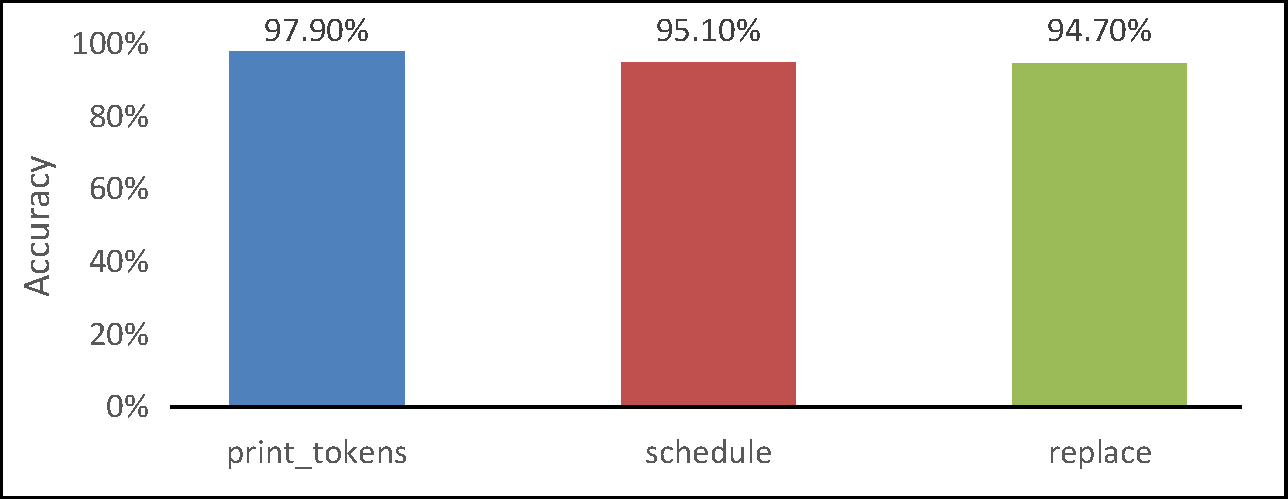
\includegraphics[width=5in]{../issta_profile/profiling/figures/overall-correctness}
\caption{Average accuracy per benchmark.}
\label{fig:overall_correctness}
\end{figure}

\subsection{Results}

To quantify \zop's accuracy, we first determined the path taken for each profiled input (\ie the ground truth) by measuring the correct profiling information for each benchmark and each input in the profiling set. Because \zop\ estimates profiling at the acyclic-path level, we used the approach by Ball and Larus~\cite{Ball:1996:EPP:243846.243857} to compute this information. Next, we performed \zop's Training~1, Training~2, and Profiling phases. For each benchmark and each profiled input, \zop\ predicted the number of times each acyclic path was executed, and we compared this value with the previously computed ground truth. We then calculated the average accuracy for each benchmark using the following formula:

\[\textrm{accuracy} = \frac{\sum_{i=1}^{n}g_{i} a_{i}}{\sum_{i=1}^{n}g_{i}}\]

where 
% SPACE
\begin{align*}
  n = & \textrm{~number of acyclic paths per benchmark.} \\
  g_i = & \textrm{~actual number executions of acyclic path~} i
          \textrm{(ground truth)}. \\
  z_i = & \textrm{~\zop~(predicted) number of executions of acyclic path~} i. \\
  a_{i} = & \textrm{~min} \Big (\frac{g_i}{z_i}, \frac{z_i}{g_i} \Big)
            = \textrm{~accuracy for acyclic path~} i. \\
\end{align*}

Therefore, when \zop\ underestimates the number of executions of a path, the accuracy is computed as $a_i = \frac{z_i}{g_i}$, whereas when \zop\ overestimates the number of executions of a path, the accuracy is computed as $a_i = \frac{g_i}{z_i}$. $a_i = 0$ when $z_i=0$. To give equal weight to each path execution, each $a_i$ is weighted by $g_i$.

Figure~\ref{fig:overall_correctness} shows the path profiling accuracy results. As the table shows, \zop's estimates are fairly accurate.  On average, \zop\ correctly predicts 94.7\% of the paths for replace, 97.9\% for print\_tokens, and 95.1\% for schedule. In other words, the profiling information computed by \zop\ \textit{without any instrumentation} is always over 94\% accurate.

Determine how the coverage of training inputs affects ZOP's accuracy, we computed how the accuracy of \zop's path count estimates is affected by the number of times each path is exercised by the training set. We show these results in Figure~\ref{fig:all_benchmarks}.  Each data point in this figure represents the accuracy of \zop's estimate for a single static acyclic path in the indicated benchmark (\ie a single $a_i$ value). For each benchmark, the figure also shows a fit for a saturating power curve\footnote{The curve is $y=a-bx^c$ where $x$ is the number of dynamic instances, $y$ is accuracy, and $a$, $b$, and $c$ are constants chosen (for each benchmark separately) to produce the best fit.} for each benchmark and the curve's goodness of fit (\ie $R^2$). We chose this type of curve because, among all simple curves we tried, including linear, quadratic, exponential, etc. it produces (by far) the best goodness-of-fit.  A logarithmic scale is used for the x-axis to more directly show the effect of increasing the number of training path instances by an order of magnitude.

\begin{comment}
\begin{figure}[htb]
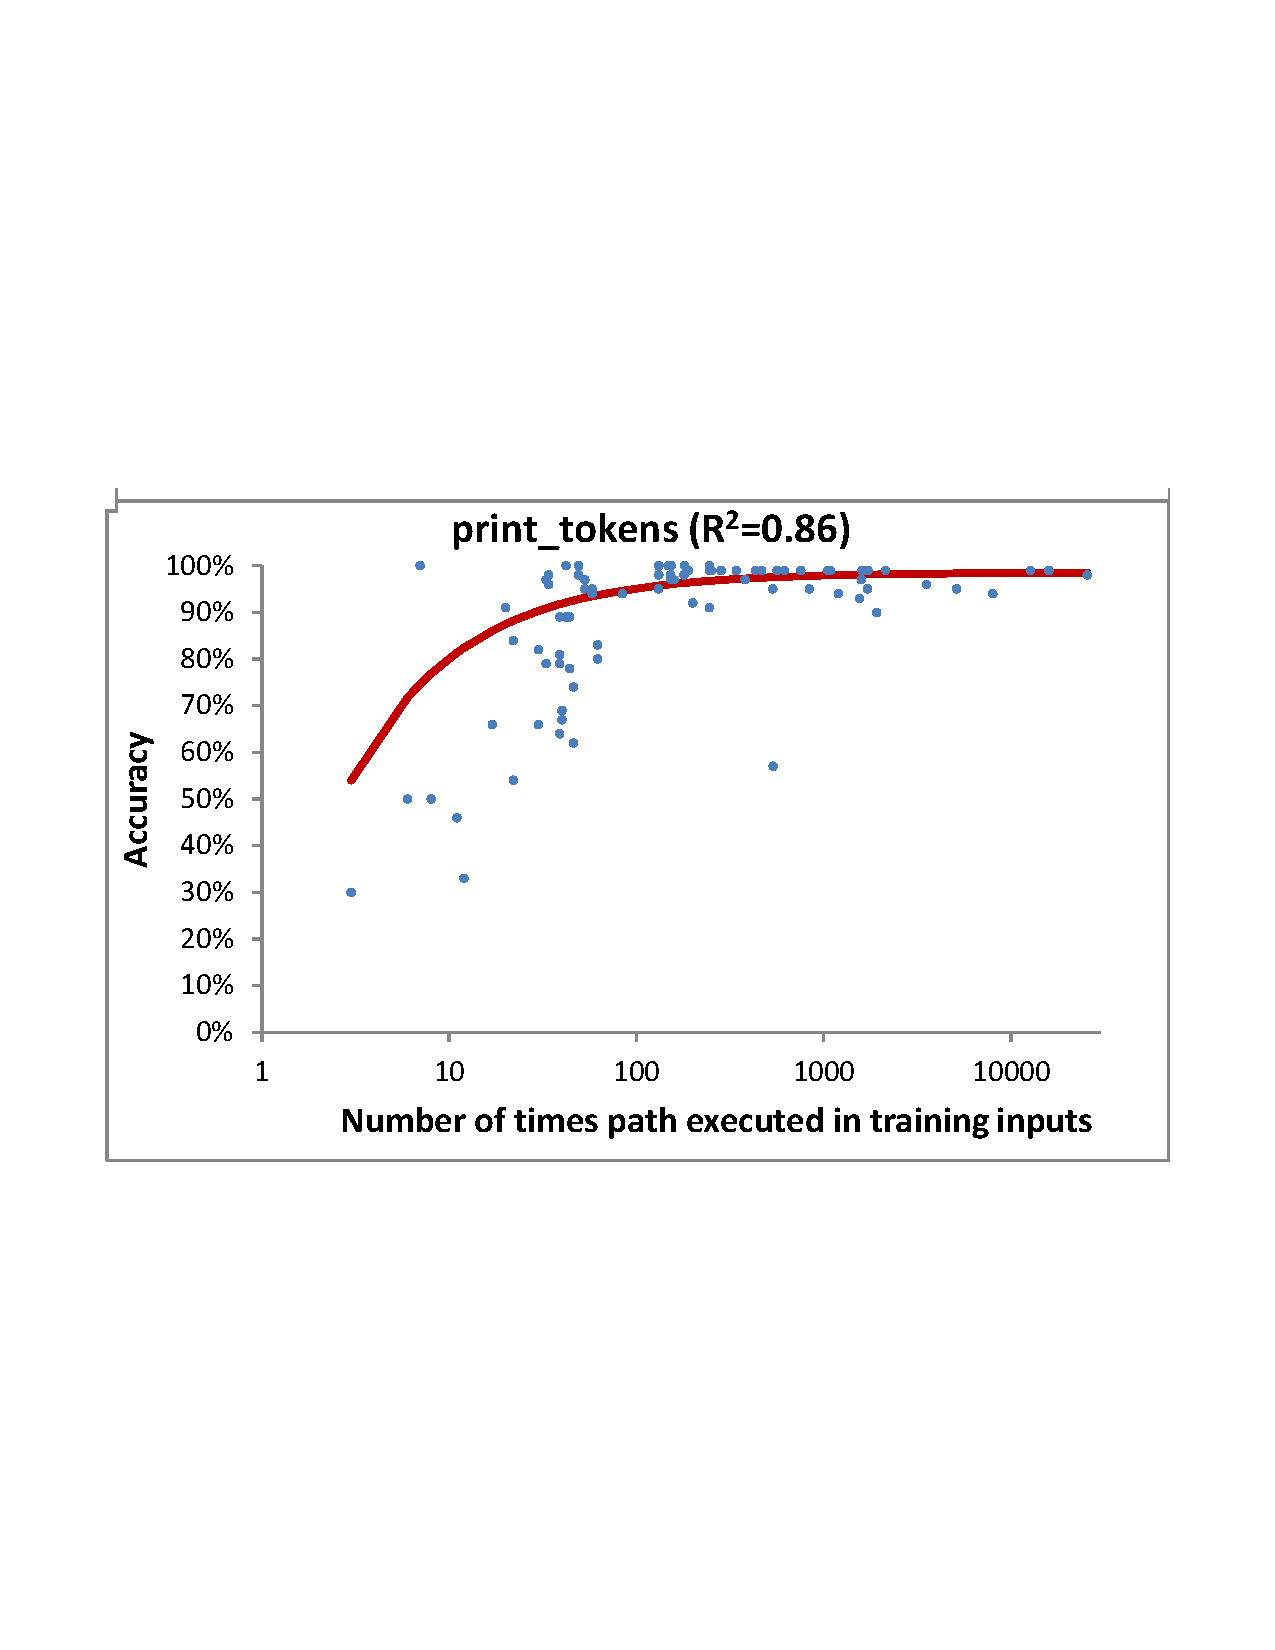
\includegraphics[width=5in]{../issta_profile/profiling/figures/print_tokens}
% SPACE \caption{Effect of the number of training examples on accuracy for print\_tokens.}
\caption{Number of training examples vs accuracy for print\_tokens.}
\label{fig:print_tokens}
\end{figure}

\begin{figure}[hbt]
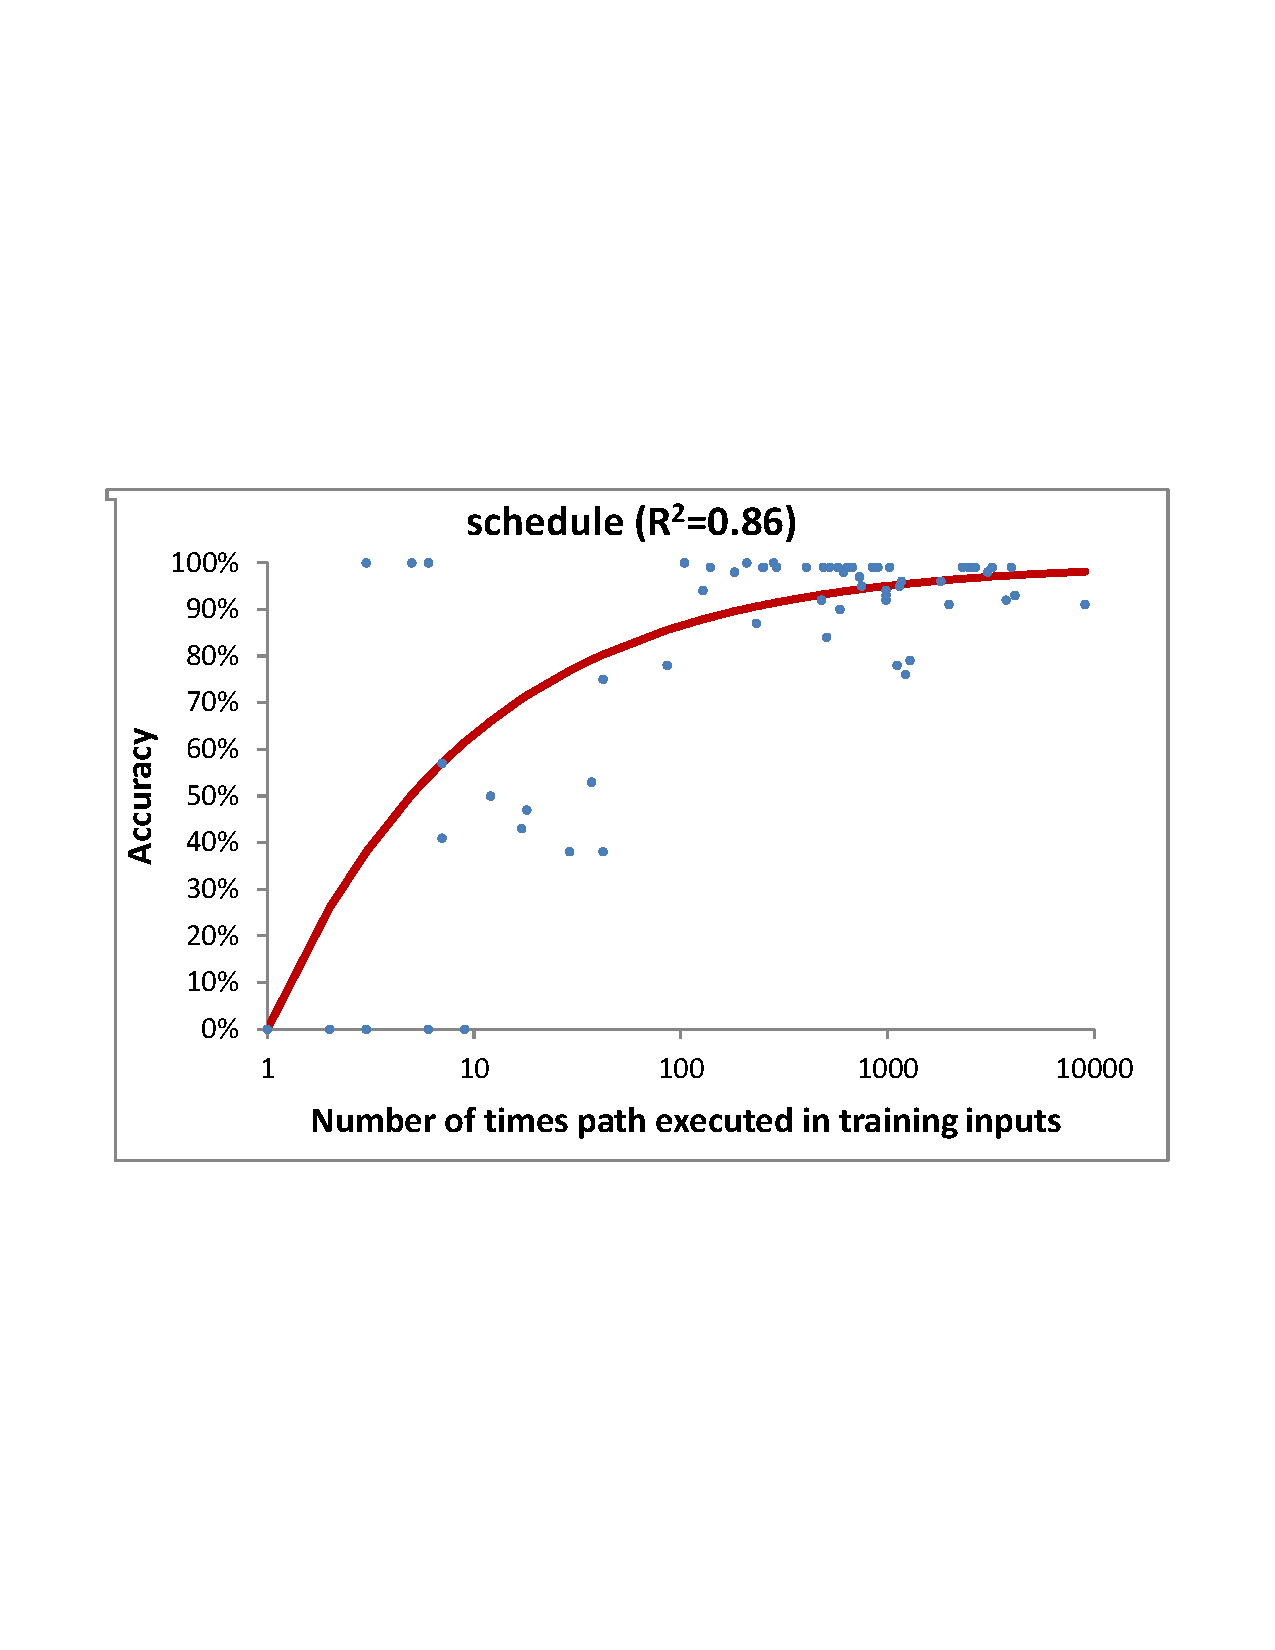
\includegraphics[width=5in]{../issta_profile/profiling/figures/schedule}
%\caption{Effect of the number of training examples on accuracy for schedule.}
\caption{Number of training examples vs accuracy for schedule.}
\label{fig:schedule}

\end{figure}

\begin{figure}[hbt]
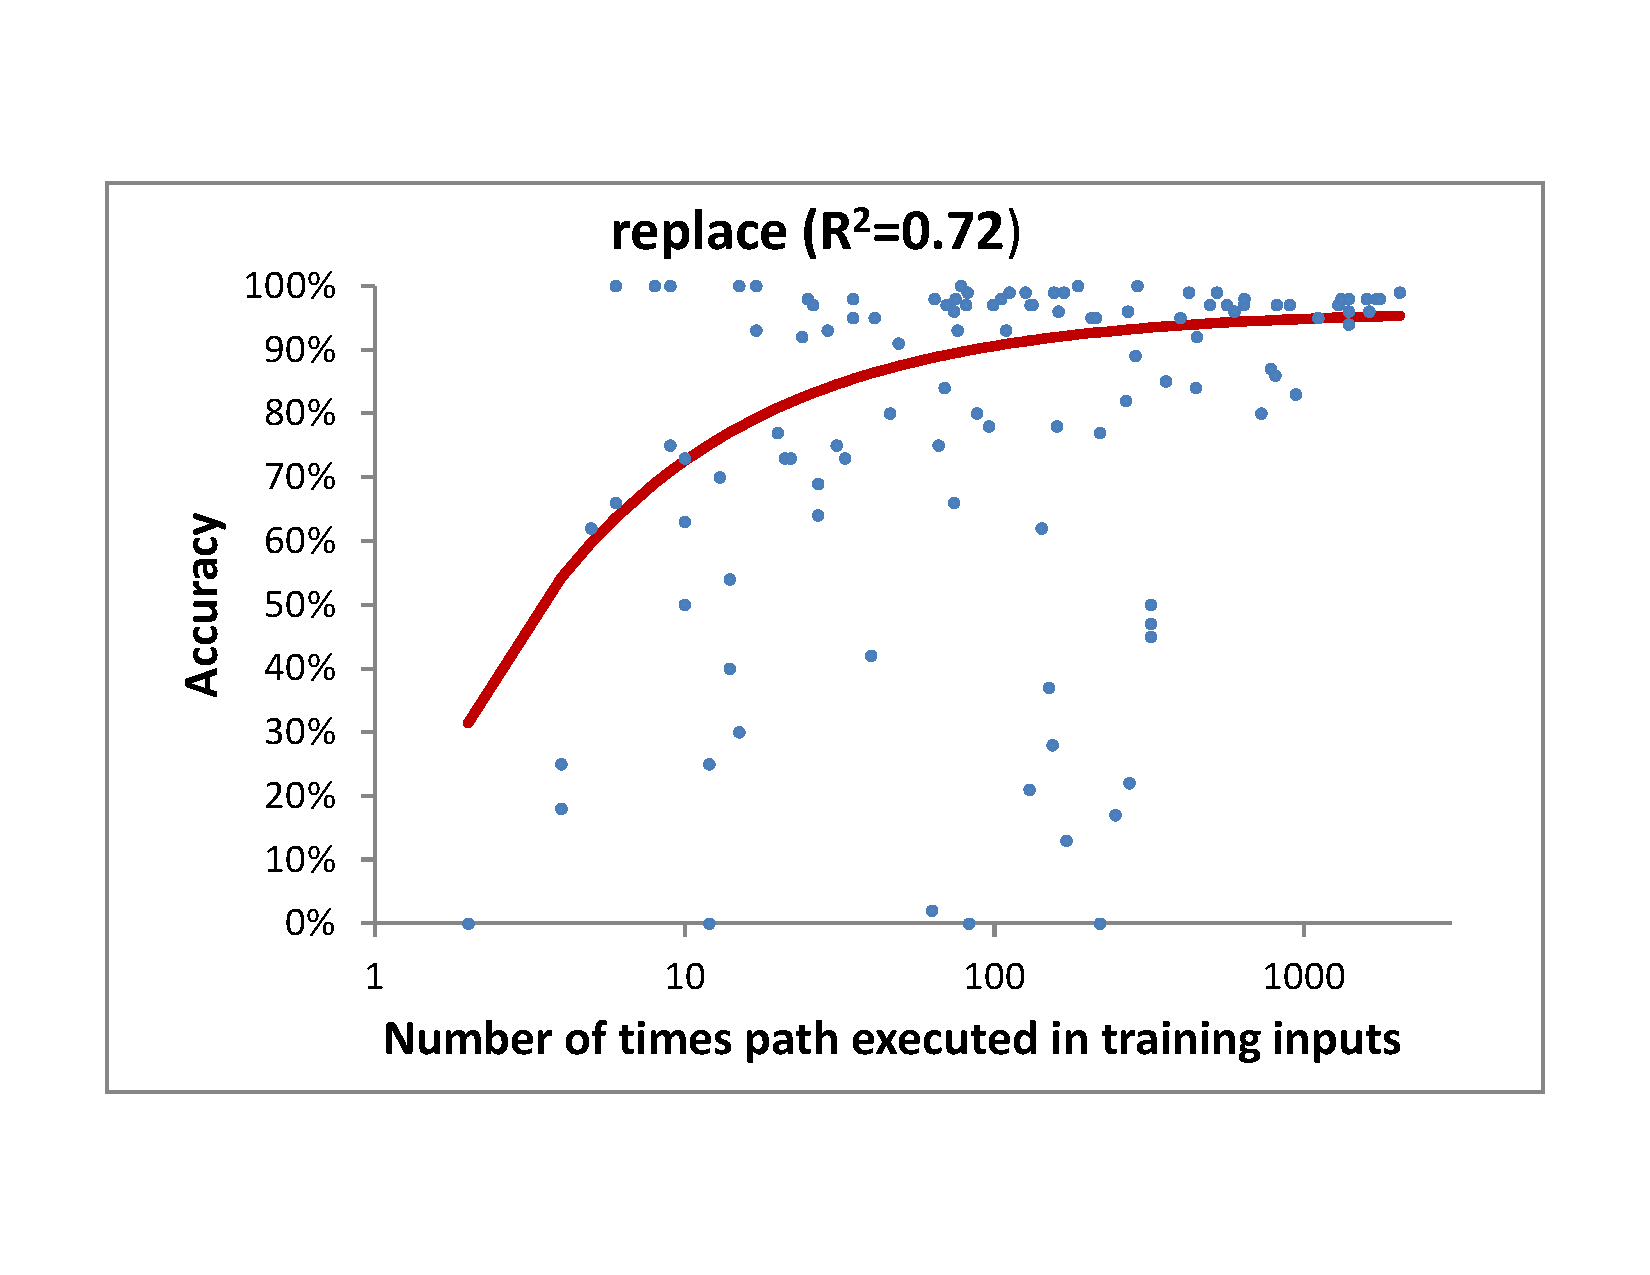
\includegraphics[width=5in]{../issta_profile/profiling/figures/replace}
% SPACE \caption{Effect of the number of training examples on accuracy for replace.}
\caption{Number of training examples vs accuracy for replace.}
\label{fig:replace}
\end{figure}
\end{comment}


\begin{figure*}[bt]

\includegraphics[width=\textwidth]{../issta_profile/profiling/figures/all_benchmarks}
% SPACE \caption{Effect of the number of training examples on accuracy for replace.}
\caption{Number of training examples vs accuracy for print\_tokens, schedule, and replace.}
\label{fig:all_benchmarks}
\end{figure*}

For the print\_tokens and schedule benchmarks in Figure~\ref{fig:all_benchmarks}, the accuracy is poor when the acyclic path is executed less than 100 times, but greatly improves beyond this point.  In fact, the vast majority of paths with more than 100 occurrences during training have nearly perfect accuracy.  This is promising, as it implies that paths can be identified accurately by a relatively small number of inputs that cover them. Moreover, it also implies that accuracy can be improved by adding more training inputs.  Finally, as we said in Section~\ref{sec:evaluation-setup}, even executions of individual procedures by means of unit tests (which are easier to create) should be sufficient for training.

The replace benchmark manifests a slightly different behavior. While the accuracy does increase with the number of times the paths are covered during training, there are several paths with more than 100 training examples that have accuracy below 80\%, and even a few below 50\%. In general the accuracy for replace does not improve as quickly as for the other two benchmarks as a function of the number of executions of a path during training.

We investigated this difference in behavior and found several possible explanations. First, whereas we expect most paths to have only so many variations in terms of the EM emanations that they can generate (see Section~\ref{zop-background}), some paths may vary more widely based on the context in which they are executed. Alternatively, some paths may simply have more possible contexts under which they can be executed (\eg if the structure of the program or some parts thereof contains especially high levels of nesting).
% I removed the discussion about interprocedural because it did not
% convince me and, moreover, contradicted the idea of using unit
% tests, which I believe can be promising...

Second, the path prediction algorithm traverses a program's marker graph as shown in the example in Figure~\ref{fig:backtracking}. This traversal results in the evaluation (and possibly selection) of many impossible paths. The technique that we use to navigate the graph is context sensitive but does not distinguish between different call sites that invoke the same callee from within a procedure. Therefore, the algorithm could reach a callee from a given call site within a procedure and return to a different call site within the same procedure. This is particularly problematic in programs in which this situation occurs frequently and may lead to imprecision and poor predictions.
%(the above issue does clearly impact performance). If further investigation confirms that this issue is indeed present, we will suitably increase the precision of our algorithm.

Finally, for 3 of the 400 inputs in replace's profiling set, the path prediction algorithm got ``lost'' while exploring the marker graph. As we mentioned while describing our approach, if the waveforms collected during training do not closely match the waveform collected during profiling for more than a short time, the predicted and actual control flows can diverge beyond recovery. Once this happens, the remainder of the prediction for that input is completely incorrect. This condition only happened for the replace benchmark and only for three inputs. This is likely an indication that there is something different about replace and that more training inputs were needed for certain parts of this benchmark. Also in this case, we will perform further investigation to better characterize the peculiarities of replace and use our findings to improve \zop.


\section{Summary}
This chapter presented \zop, a system for zero-overhead profiling which is non-intrusive and requires no hardware modifications or support. In exchange for the ability to profile software without any overhead, \zop\ makes a small sacrifice in accuracy ($>$ 94\% accurate compared to a technique based on instrumentation on the benchmarks tested), and requires a training phase.

\zop\ uses unintentional EM emanations generated by the profiled system to track a program's execution and to generate profiling information. In \zop's training phase, the program is instrumented and EM waveforms are recorded while running a set of inputs on both instrumented and uninstrumented code, and the instrumentation records which part of the EM signal corresponds to which part of the code. The profiling phase consists of running the original (uninstrumented and unmodified) program with the inputs to be profiled and recording the system's EM emanations waveforms. The waveforms from training, and their waveform-to-code mapping, are used to predict the execution path taken by the profiled run. Our experimental results show that \zop\ can predict profiling information with greater than 94\% accuracy for the benchmarks considered in our evaluation.



\chapter{Detection of Unknown Code on Internet of Things Devices at a Distance}
\label{sec:malware_detect}

\section{Overview}
\label{malware-dist-overview}
One of the emerging applications that makes use of the information embedded in EM emanations is the verification of control flow through a program, specifically the detection of previously unseen (i.e. zero day) malware. A rapidly growing number of embedded devices with internet connectivity are used in consumer electronics, Internet of Things devices, as well as industrial control and data acquisition applications. Securing these devices presents new and unique challenges due to their very limited software and hardware resources, the difficulty of applying software updates in the field, and the lack of standardization among the many hardware and software platforms used across devices. Techniques that make use of EM emanations to secure these devices may be a good fit for this application because such techniques do not require intrusive access or modification to the devices, and because remotely monitoring the devices in an air-gapped manner makes it impossible for an attacker to hide malicious activity by disabling security measures on the compromised device. Another advantage of using EM emanations to detect malware is that this detection can be done ``wirelessly,'' since it does not require a physical connection between the monitor and the monitored device. A single monitor could potentially observe the EM emanations from all the computing devices in a room and simultaneously secure all of them. Therefore we need to determine how strong the relevant EM emanations from the monitored devices are and how much distance can separate the monitor and the monitored devices while still accurately detecting malware. 

This chapter adapts ZOP for detecting malware, characterizes the effects which degrade ZOP's performance when monitoring devices from a distance, and shows results for detecting malware using ZOP at distance of 3 meters. Section~\ref{adapt_zop} describes how we can apply the algorithms developed for ZOP to detect malware. Section~\ref{malware-dist-static} examines the effect that microarchitectural events have on prediction accuracy by presenting a comparison of ZOP's whole program path prediction accuracy between NIOS and PIC32 processors. Section~\ref{malware-dist-snr} presents measurements that describe the effect on ZOP performance of using EM emanations at different clock harmonics, as well as the impact of using different antennas, signal bandwidths, and measurement distances, and defines a signal quality metric for ZOP. Section~\ref{malware-dist-detect} presents measurement results for detecting unknown code in executions of a known program at a distance of 3 meters, and Section~\ref{malware-dist-summary} summarizes this chapter. 




% edit distance, pic32
\section{Adapting ZOP to Detect Malware}
\label{adapt_zop}

In Chapter~\ref{zop}, ZOP profiled devices using a small EM probe very close to the device being profiled. This chapter builds on ZOP and addresses two new requirements: (1) in addition to predicting the most likely control flow path through a program, predict whether ``unknown'' code (e.g. malware) executed, and (2) do this prediction from a distance of 3 meters. Chapter~\ref{zop} measured the average accuracy of counts of all the dynamic occurrences of acyclic intraprocedural paths in a program across a set of inputs. That metric is only useful for path profiling, but for other applications such as malware detection, we will need a new metric which can be used to measure whole program path prediction accuracy. When determining whole program path prediction accuracy, we have two paths to compare. The first path is the sequence of basic blocks that the program actually executed for a given input (call this sequence $S$), and the second is the sequence of basic blocks that ZOP predicts for that same execution (call this sequence $T$). One efficient method of comparing two sequences of symbols is the string edit distance which we will call $d(S,T)$. The string edit distance is a single number which is the total edits necessary to transform sequence $S$ into sequence $T$. This transformation consists of a sequence of edits where each edit consists of deleting a single symbol from $S$ or adding a single symbol to $S$. The edits are applied iteratively to sequence $S$ until the sequence $T$ is produced, and the edit distance is defined as the minimum number of edits necessary to transform $S$ into $T$. In this formulation, each unique basic block is a symbol. In this chapter we will use the unique markers as symbols for convenience and because we only have the timing of the markers (not the basic blocks) in the observed waveforms. This ``marker edit distance'' can be converted to a fraction by calculating $\frac{d(S,T)}{|S|}$. This fraction indicates the percentage of the program whose path was mispredicted, and the whole program path prediction accuracy will be calculated as $1 - \frac{d(S,T)}{|S|}$. This metric is useful for summarizing whole program path prediction accuracy for a given execution and for isolating the time periods where the predicted path is incorrect in a particular execution. Both of these are important tools for understanding path prediction accuracy.

To understand how ZOP can be adapted to detect malware, consider how ZOP would behave when it attempts to predict the control flow path through a program when unknown code (malware) is present. For our purposes, we will focus on unknown code, i.e. any code which we haven't observed as part of the monitored program during training. This unknown code could be part of any type of malware that results in the execution of code not present in monitored program, such as a buffer overflow attack or a clandestine malicious modification to the program. When we use ZOP to predict the path through a program where unknown code is present, ZOP will accurately predict the path through the program for the portions of the execution where the known code is active. For the portions of the program where unknown code is active, ZOP attempts to match the EM emanations waveforms generated by the unknown code to the training waveforms for the known program. If the unknown code is active for a long enough period of time, the execution of this unknown code is virtually guaranteed to generate EM emanations waveforms which match the training waveforms quantifiably worse than any valid execution of known code in the monitored program. In other words, when malware is present the received signal will not match any training examples resulting in low confidence in the path prediction results since the malware will not correspond to any valid program path. Therefore high accuracy malware detection requires ZOP to not only predict the execution path correctly, but also requires that the training and execution waveforms match (e.g. correlate) with high confidence when known code executes.

\section{ZOP Whole Program Path Prediction Accuracy on NIOS and PIC32 Processors}
\label{malware-dist-static}
In this section, we will use ZOP to predict the whole program path on the NIOS processor (used in Chapter~\ref{zop}) and also on a simpler PIC32 processor. The NIOS processor uses an external memory and has on-chip data and instruction caches which introduce microarchitectural event differences (such as cache hit/misses) among dynamic instances of a given static path. The Microchip PIC32MX795F512L is a 32 bit, 80 MHz processor with similar architecture to NIOS, with the main difference being that it uses neither external memory nor on-chip instruction and data caches. This difference is important, as the lack of a cache and external memory greatly minimizes the effect of processor microarchitectural event differences when executing a given static path. On the PIC32 processor, repeated executions of a given static path will execute in nearly the same number of clock cycles and the EM emanations waveform for each dynamic instance of a single static path are highly correlated to one another. To remove any effects caused by differences in processor/memory clock rates between the processors, for all the measurements in this chapter we set the NIOS processor and memory clock rate to 83.333 MHz (this is the closest FPGA PLL frequency available near the PIC32's 80 MHz clock rate). Any difference in ZOP's performance between these two processors is likely due to microarchitectural event variations present only in the NIOS processor, since this is the key difference between the two processors. Other signal effects (noise, signal propagation, etc.) will be minimal and equivalent between the two processors because they will be measured under the same conditions. 
%Therefore, differences in performance between measurements on the PIC32 and NIOS processors are likely ca.

\begin{table}[hbt]

\includegraphics[width=5in]{pic32_performance}
\caption{A comparison of ZOP's whole program path prediction performance on the PIC32 and NIOS processors for the replace benchmark measured using the marker edit distance ratio.}
\label{pic32_performance}
\end{table}

To evaluate the difference in ZOP's whole program path prediction performance on the NIOS and PIC32 processors, the replace benchmark was run using the same sets of training and evaluation inputs and same measurement setup (i.e. a small tuned LC probe very close to the monitored processor) as described in Chapter~\ref{zop}. Table~\ref{pic32_performance} shows a performance comparison using the marker edit distance ratio metric described in Section~\ref{adapt_zop}. The whole program path was predicted exactly or almost completely correctly for vast majority of the inputs (those with marker edit distance ratio less than 0.01). For 6 evaluation inputs on the PIC32 and for 18 evaluation inputs on NIOS, the marker edit distance was very large ($>$ 0.25). The performance on these inputs was investigated, and it was found that for almost all such inputs the execution was very short ($>$ 10 markers long), so that missing only a few markers resulted in a large marker edit distance ratio. For 3 of the executions with a large marker edit distance ratio the executions were, however, sufficiently long that we can conclusively say that ZOP completely failed and lost track of the actual execution path. After investigation, it was determined that these inputs all got lost in the function shown in Figure~\ref{replace_omatch}.

\begin{figure}[h]
  \centering
\lstset{language=C++,basicstyle=\ttfamily\scriptsize,numbers=left}\lstset{escapeinside={/*@}{@*/}}
\begin{lstlisting}[frame=none,xleftmargin=30pt]
int omatch(char *lin, int *i, char *pat, int j) {
  char advance = -1;
  bool result;
  mark(A);
  if (lin[*i] == ENDSTR) result = false;
  else if (!in_pat_set(pat[j])) {
    return false;
  } else {
    switch (pat[j]) {
    case LITCHAR:
      if (lin[*i] == pat[j + 1]) advance = 1;
      break;
    case BOL:
      if (*i == 0) advance = 0;
      break;
    case ANY:
      if (lin[*i] != NEWLINE) advance = 1;
      break;
    case EOL:
      if (lin[*i] == NEWLINE) advance = 0;
      break;
    case CCL:
      if (locate(lin[*i], pat, j + 1)) advance = 1;
      break;
    case NCCL:
      if ((lin[*i] != NEWLINE) && (!locate(lin[*i], pat, j + 1))) {
        advance = 1;
      }
      break;
    default:
      Caseerror(pat[j]);
    }
  }
  if ((advance >= 0)) {
    *i = *i + advance;
    result = true;
  } else {
    result = false;
  }
  mark(B);
  return result;
}
\end{lstlisting}
\caption{A function which had poor static path coverage in the replace benchmark.}\label{replace_omatch}
\end{figure}

The function in Figure~\ref{replace_omatch} only has two markers, one at the start and one at the end of the function. Without the basic block sequence information for each dynamic path, it is impossible to determine the path coverage of the training set. However, the number of possible paths through this function is large, and given the criteria used to select the training inputs in Chapter~\ref{zop}, it is expected that many of the marker-to-marker paths through this function are not present in the training set. Based on this comparison, we propose that this training set has mostly adequate coverage of the marker-to-marker static paths with a few such exceptions. Furthermore, it was observed that repeated executions of replace with the same inputs and initial cache state showed very little variability in the EM emanations waveform (see Section~\ref{malware-dist-snr} for more information), so the effects of signal propagation, noise, and other distortions was negligible for this measurement setup. We conclude therefore that the decreased performance on NIOS (compared to PIC32) is due to microarchitectural variation (e.g. variation introduced by the external DRAM and on-chip caches), since all other effects should be the same between the NIOS and PIC32 measurements.





\section{Quantifying Signal Quality as a Function of Antenna, Frequency, and Distance}
\label{malware-dist-snr}
In Chapter~\ref{zop} we used a tuned LC circuit placed directly above the processor's bypass capacitors as a probe to receive the modulated processor clock signal at $f_c = 50$ MHz. In this chapter we use a processor clock frequency of $f_c = 83.333$ MHz. The signal received with this setup is very strong and essentially free from noise and interferences. However, at this frequency and distance, the probe is in the near field and so the received signal decays quickly as the distance is increased, so that at a distance of a few centimeters the signal amplitude is too low to be used. At the processor frequency (83.333 MHz), our target distance (3 meters) is still not in the far field and so a sophisticated (and likely very large) near field probe would be needed to provide a strong enough signal. The processor and memory clocks are roughly square waves, and so EM emanations are generated at the harmonics (multiples) of the processor clock frequency. As the frequency increases the minimum far field distance decreases and compact high gain antennas can be used, so we will attempt to demodulate and characterize these clock harmonics. 

Before using ZOP at a distance, we characterized the signals ZOP uses, focusing on the signal effects which change as a function of the distance, antenna, and the harmonic used. First, we characterized the strength of the carriers and modulated signals generated at the harmonics of the processor clock. To do this, we first need a modulation signal (i.e. system activity) which is easy to control and measure. The LDM/LDL1 (Load from Memory vs Load from L1 Cache) SAVAT benchmark generates a narrow peak in the sideband of all the carriers modulated by this activity. In this experiment, modulated carriers exist at all the harmonics of the processor clock (e.g. the first harmonic at 83.333 MHz, the second harmonic at 166.666 MHz, etc.). For each of these carriers, we made 6 measurements. First we measured the power of the signal generated at the carrier, where the carrier occurs at frequency $f_h = h f_1$ where $f_1 = 83.333$ MHz. Then we measured the power of the SAVAT modulation signal occurring in the right and left sidebands at $f_h \pm f_{alt}$ where $f_{alt} = 100$ kHz (the SAVAT alternation frequency). The power is integrated across a 10 kHz band centered at the frequency of interest to allow for any spread or variation in the frequency of the generated sidebands. First we do each of these measurements with the FPGA powered on and SAVAT running. Next, we power off the FPGA and remeasure the signal power at $f_h, f_h - f_{alt}, f_h + f_{alt}$ again to get an indication of the ambient noise at these frequencies. We performed each of these measurements at the harmonics from $h = 1$ (83.333 MHz) to $h = 43$ (3.5833 GHz). We use a Com-Power AH-118 broadband double ridge horn antenna, which has a relatively flat frequency response from 700 MHz to 18 GHz and 10 dBi gain over this frequency range. The signal was recorded using the same N9020A MXA spectrum analyzer as in previous experiments. The distance between the FPGA board and the antenna was 60 cm.

In Figure~\ref{savat_harm_mag}, each line shows the power measured at the carrier and sideband frequencies with SAVAT active minus the power at these same frequencies with the FPGA powered off. Note that we can only measure these quantities at the frequencies that are harmonics of the clock, so for each trace, there are 43 evenly spaced data points (for harmonics $h = 1$ to $h = 43$). A line is drawn connecting these points to indicate the general trend in power as a function frequency. As shown in the figure, the left and right sidebands have comparable powers. This is expected because the distance between the right and left alternation frequency is only $2 f_{alt} = 200$ kHz and the frequency response of the channel is expected to be flat over such a narrow span. The power of the SAVAT signals is approximately 20 dB above the noise floor for most frequencies, indicating a strong (usable) signal exists at many harmonics. Most interestingly, the power of the carriers and sidebands does not decay significantly as frequency increases. While the higher order harmonics of an ideal square wave decay quickly as a function of frequency, the signal received in this setup is affected by several additional factors. First, the currents and voltages generated within the FPGA, DRAM, and PCB at the carrier and modulation frequencies will vary greatly as a function of frequency. Also, for a current of a given magnitude flowing through a wire on a PCB, a stronger EM field will be generated as the frequency of the current increases. 

\begin{figure}[hbt]
\includegraphics[width=5in]{savat_harm_mag}
\caption{Magnitude of processor clock harmonics 1 through 43 as carriers and as modulated by 100 KHz SAVAT LDM/LDL1 activity.}
\label{savat_harm_mag}
\end{figure}

To reliably receive the signals ZOP uses, we need to pick a frequency range where antennas with high gain can be found. We chose the 2.3 GHz - 2.7 GHz frequency range because it is widely used for wifi and other wireless protocols, and so many high gain commercial antennas are available. For several antenna types and carriers (harmonics) in this range we measured the EM emanations while executing the replace benchmark repeatedly with the same inputs. In Chapter~\ref{zop} we found that simple AM demodulation (i.e. simply taking the magnitude of of the IQ signal for the 8.333 MHz band around the carrier) resulted in a very strong signal with very little noise when using the tuned LC inductor probe at 83.333 MHz. Repeated executions of the benchmark for this setup resulted in demodulated waveforms with almost no noise, so that there was very little signal variation between repeated executions of a program with the same inputs. However, when we demodulated the harmonics similarly with several different types of antennas and frequencies in the 2.3 GHz - 2.7 GHz band, we found that there was little relation between the SAVAT power in Figure~\ref{savat_harm_mag} and the signal strength in demodulated waveforms for a given frequency and antenna. 

This variation in the signal strength relative to SAVAT power was determined to be caused by the nature of the unintentional modulation of signals within computer systems. In modern communications systems, the transmitter minimizes the power wasted on the continuous wave carrier to order to maximize the power available to modulate the carrier and transmit information. Furthermore, the phase and magnitude of the transmitted signals are carefully controlled to maximize data transfer rates. Unintentionally modulated computing signals (such as processor clocks) are not designed as carriers, and so do not have either of these two properties. First, a large portion of the transmitted power is not modulated. For example, the power consumed by a processor as it executes a program may vary during different portions of a program, but there is a non-zero minimum amount of power consumed by the circuitry on the processor clock, and this minimum can be on the order of the variations in power usage over the execution of a program. Second, different circuitry driven by the same clock may not all share a common phase (for example there may be a phase difference between the processor and memory activities even when they share the same clock), and similarly it is plausible that delays through the power distribution network could result in phase variation in the current drawn (and therefore cause phase variations in the EM emanations). 

%could potentially have additional sources (maybe show example)

Previously we used asynchronous AM demodulation, but to understand these modulation effects we first applied carrier recovery to compensate for the small frequency offset between the receiver (the spectrum analyzer) and transmitter (the computing device under test). After this, the unexplained variation in the signal strength was obvious and can be explained by Figure~\ref{multiple_clock_components}. We hypothesize that the EM emanations from a computing device can be modeled as $s(t) = C e^{jwt} + M(t) e^{j\cdot(wt+\phi)}$ where the first component $C e^{jwt}$ is a sinusoid at the carrier frequency $w$ with real magnitude $C$ and the second component $M(t) e^{j\cdot(wt+\phi)}$ is at the same carrier frequency $w$ but has modulated magnitude $M(t)$ and a phase offset $\phi$ relative to the first component. Based on these assumptions, after carrier recovery (e.g. in the simplest form, multiplying $s(t)$ by $e^{-jwt}$) we would expect the AM modulated component to be offset from the origin by $C$ and rotated by $\phi$ in an IQ plot. Figure~\ref{all_iq_h31} shows IQ plots for demodulated signals after carrier recovery for the 31st harmonic at 2.58 GHz with several antennas and antenna orientations. The upper left plot shows the demodulated data for a H field probe placed directly on top of the FPGA. The remaining plots were measured at a distance of 60 cm. The bottom left plot shows results for a helical antenna. The other plots show results for the same 10 dBi horn antenna used before, and an L-com HG2418P 2.4 GHz 18 dBi directional panel antenna, with two plots each showing two orthogonal orientations. For each of these measurements, a low noise amplifier with a 1 dB noise figure and 20 dB of gain was placed between the antenna and spectrum analyzer. Each dot in a plot represents an IQ sample in the demodulated waveform recorded during execution of the replace benchmark with the same inputs after carrier recovery. The large red X marks the origin (i.e. $I=0, Q=0$). The mean IQ value across all the samples for a given plot is different in each plot, and the dominant variation axis is rotated by varying angles between the plots. These results agree with the hypothesis that the EM emanations at the processor/memory clock frequency consists of two components: one unmodulated, and one modulated and rotated by angle $\phi$.

\begin{figure}[hbt]
\includegraphics[width=5in]{multiple_clock_components}
\caption{A diagram illustrating an IQ plot for an unintentionally modulated signal with two synchronous components (one modulated, one not modulated) with the same frequency but different phases.}
\label{multiple_clock_components}
\end{figure}

\begin{figure*}
\includegraphics[width=\textwidth]{all_iq_h31}
\caption{IQ plots for the modulated 31st clock harmonic with several antennas and orientations.}
\label{all_iq_h31}
\end{figure*}

Based on these measurements and analysis it is clear why the demodulated signal strength is not directly related to the measured SAVAT power. Depending on the phase offset $\phi$, more or less of the signal is captured by AM demodulation. For example, as shown in Figure~\ref{all_iq_h31}, if we demodulate by simply taking the magnitude of each IQ sample we will capture a small fraction of the signal when using the H field probe signal but will capture a much larger (though still not optimal) fraction of the signal for the helical antenna. It is important to note that some portion of the signal is present in the variation orthogonal to the main axis of modulation. In other words the signal is phase modulated in addition to being AM modulated. Regardless of the choice of offset and axis for AM demodulation, repeatable patterns are present in the phase of the IQ samples as a function of time across repeated executions of the same program and inputs. Therefore AM demodulating the signal throws away some usable signal. This repeatable phase variation might be explained by the fact that there are many small circuits drawing current with slightly different phases when they are active resulting not only a continuous range of amplitudes but also a continuous range of possible phases. It is also likely that the channel's frequency response is not completely flat. This can contribute to repeatable phase variation even for purely AM modulated signals. %For example, we might expect no signal or pattern in the phase as a function of time after doing simple AM demodulation of the signal show in the IQ plot for the horn antenna in the horizontal orientation. However, Figure~\ref{

\begin{figure*}
\includegraphics[width=\textwidth]{panel_iq_hx}
\caption{IQ plots for several harmonics using the 18 dBi panel antenna with horizontal orientation.}
\label{panel_iq_hx}
\end{figure*}

It is also interesting to compare IQ plots for multiple harmonics of the same processor clock signal. Figure~\ref{panel_iq_hx} shows IQ plots for several such harmonics using the same panel antenna at a distance of 60 cm. In terms of the demodulated waveform shape in the time domain, from theory we would expect the demodulated signals from different harmonics of the same clock to have the same shape. Figure~\ref{panel_abs_hx} shows that this is largely true. This is significant because it suggests signals from multiple harmonics can be combined together to increase the signal strength and to overcome interferences in individual harmonics. 

\begin{figure*}
\includegraphics[width=\textwidth]{panel_abs_hx}
\caption{Demodulated and normalized time domain signals for several harmonics using the 18 dBi panel antenna with horizontal orientation.}
\label{panel_abs_hx}
\end{figure*}

Finally, we are interested in how the signal decays with distance. Figure~\ref{panel_abs_h31_cm} overlays the demodulated time domain signal for 10 repeated executions of the same benchmark with the same inputs for the 31st harmonic, comparing the waveform shape at 60 cm and 300 cm. While the signal magnitude is slightly lower at 300 cm, the overall waveform shape is similar for these two distances. 

\begin{figure*}
\includegraphics[width=\textwidth]{panel_abs_h31_cm}
\caption{IQ plots for 10 repeated runs of the same benchmark and inputs for the 31st harmonic at 60 cm (top) and 300 cm (bottom)  using the 18 dBi panel antenna with horizontal orientation.}
\label{panel_abs_h31_cm}
\end{figure*}

%carrier tracking
%removing complex offset

In order to begin to understand how signal quality for a given environment (i.e. antenna, amplifier, distance, etc.) can affect ZOP's performance, we first need a metric to quantify the ``usable'' signal strength. Some methods for quantifying average signal strength require significant control over the signals generated by the transmitter, or theoretical assumptions about the transmitter. It is not obvious how to apply these methods to our scenario, as the only control we have is the ability to generate the same pattern repeatedly by executing the same benchmark with the same inputs and observing variation in this signal. Any feature of the received signal which is common between all the repeated executions (i.e. present in the mean across all the executions at a given time point) will be referred to as ``positively correlated'' since these features contribute to higher correlation between any two waveforms measured during repeated execution of the same code (assuming the waveforms are normalized). Any feature in the signal which is present in a single execution but not present in the mean across all repeated executions will be considered ``negatively correlated'' since such features tend to contribute to lower correlation between two waveforms measured during repeated execution of the same code.

We next define a single value that represents the average strength (magnitude) for a newly defined signal consisting of the sum of all the positively correlated features in a given set of waveforms measured during repeated executions of the same code (call this value $P$), and similarly define a single value for the average magnitude of the signal consisting of the sum of the negatively correlated features (call this value $N$). If $x[r,t]$ is the (demodulated) signal value at time $t$ of the $r$th repeated execution, then we can estimate $P$ by first taking the mean among all the repeated waveforms $x[r,t]$ at each time instant $t$ to create an average signal $p[t]$ and then taking the standard deviation of $p[t]$ across all time $t$:
\begin{equation}
\begin{aligned}
p[t] &= \textrm{mean}_r \> x[r,t] \\
P &= \textrm{std} \> p[t].
\end{aligned}
\end{equation}
$P$ is then a single value that estimates of the magnitude of the signal that is common between executions. Similarly, we can estimate $N$ as
\begin{equation}
% 2/15/2017: changed t -> r. take std() of each waveform, then mean of these stds(). same as in slides and matlab code
\begin{aligned}
n[r] &= \textrm{std}_t \> (x[r,t] - p[t]) \\
N &= \textrm{mean} \> n[r].
\end{aligned}
\end{equation}
Then a given program execution $r$ has a waveform $x[r,t]$ which can be decomposed into two signals: $p[t]$ (the signal consisting of the positively correlated features which are common between all executions) and $x[r,t] - p[t]$ (the signal consisting of the negatively correlated features present in $x[r,t]$ but in present among all the other executions). 

\begin{figure}[hbt]
\includegraphics[width=5in]{snr_distance}
\caption{A plot of the magnitudes of the positively and negatively correlated signal features as a function of distance using 18 dBi panel antenna with horizontal orientation.}
\label{snr_distance}
\end{figure}

\begin{figure}[hbt]
\includegraphics[width=5in]{snr_bandwidth}
\caption{A plot of the magnitudes of the positively and negatively correlated signal features as a function of demodulation bandwidth using 18 dBi panel antenna with horizontal orientation.}
\label{snr_bandwidth}
\end{figure}


One usage of the $P$ and $N$ values is to estimate the decay of the signal as a function of distance. This is shown in Figure~\ref{snr_distance}. In the figure, the magnitude of the negatively correlated features, $N$, is constant for a given harmonic, as would be expected for a fixed level of ambient noise. This figure also confirms that simple AM demodulation captures only a varying portion of the total signal depending on the complex offset $C$ introduced by the non-modulated component in the IQ plot together with the phase rotation $\phi$. For example, in Figure~\ref{panel_iq_hx}, the 28th harmonic has a complex offset $C$ and phase $\phi$ that results in the least fraction of the total signal being captured by simple AM demodulation, and also has the lowest signal level in Figure~\ref{snr_distance}. Similarly, the 31th harmonic's complex offset $C$ is the smallest, resulting the strongest signal level in Figure~\ref{snr_distance}. In the IQ plots in Figure~\ref{panel_iq_hx}, the area with the highest concentration of samples corresponds to the point where the modulation signal $M(t)$ is at its minimum. For these signals subtracting this offset before AM demodulating would yield the strongest signal, i.e. the signal with the largest $P/N$ value.

Figure~\ref{snr_bandwidth} shows the magnitudes of the positively and negatively correlated signal features as a function of the demodulation bandwidth (i.e. the width of the frequency band around the carrier that is demodulated) for the same demodulated harmonics and measurement setup used for Figures~\ref{panel_iq_hx} and~\ref{snr_distance}. This figure shows that the ratio $P/N$ is in fact lower at higher baseband frequencies, meaning that as we increase the demodulation bandwidth, we would expect the correlation between the training waveforms and the to-be-predicted waveforms to decrease. We confirmed this by using ZOP with different demodulation bandwidths and observing that if the bandwidth was too high, the performance suffered. The fact that $P/N$ decreases as frequency increases suggests that there is increasing time and/or amplitude variation in the waveform features generated for very rapid changes in processor activity. One explanation for this phenomenon is that for repeated executions of the same program with the same inputs, the variation in microarchitectural activity occurs on small timescales, generating high frequency features in the signal, but that it is much more difficult for microarchitectural activity to cause low frequency features. This makes intuitive sense because it is extremely unlikely that microarchitectural variation alone could cause a program to take 1 second for one execution and 2 seconds for another run of the same program, but it is plausible that microarchitectural activity could cause a section of code to take 100 clock cycles in one execution vs 200 clock cycles in another execution. 








\section{Detecting Unknown Code at a Distance}
\label{malware-dist-detect}
%picture of panel antenna setup, including amplifier
This section applies the knowledge gained in the previous section to detect the presence of unknown code at a distance of 3 meters. We used the antenna with the highest gain (the 18 dBi panel antenna) and the same replace benchmark with the same training and evaluation inputs as used in Chapter~\ref{zop}. As we determined in Section~\ref{malware-dist-static}, this training set has poor coverage of some portions of this benchmark. While it is expected that better input generation will improve ZOP's performance, but generating inputs with thorough coverage of large programs is challenging. Therefore we will continue to use this training input set because ZOP needs to be robust against training inputs that do not provide perfect coverage. 

In this measurement we will evaluate whether ZOP can predict when unknown code is present in a given program execution. For this purpose, we will not use any of the training waveforms which describe a particular function (the \texttt{putsub} function) in the replace benchmark. Therefore, when ZOP encounters calls to this function, it will attempt to match the unknown waveform to only to training waveforms for the valid known code paths, but not to the \texttt{putsub} function. These waveforms will not match well against the unknown waveform because the unknown waveforms were recorded during different program activity (i.e. the \texttt{putsub} function). In other words, the waveform matching is expected to be good when ZOP encounters known code (i.e. code for which it has training examples), and poor when ZOP encounters unknown code (i.e. code with no training examples). Therefore, if we look at the matching between to-be-predicted waveform and the training example waveforms ZOP picks as the best matches to the to-be-predicted waveform during a period of time where code is executing for which we have no training examples, we would expect that the matching will be very poor (i.e. have a low correlation). 

We can use the fact that the best matching training examples will have low correlation to unknown code to determine whether a given execution contains unknown code. To do this, for a given execution, for each predicted marker in the predicted marker sequence, we look at the correlation between the highest correlated training example waveform (which was used to selected this marker in the final prediction) and the to-be-predicted waveform. This gives us a list of correlations between the highest correlated training waveform and the to-be-predicted waveform for short sections of the waveform recorded for the entire duration of the program's execution. Then, for each executed input, we find the minimum correlation in this list, and assign that value to that executed input. This gives us a score that is likely to be lower when unknown code is present for a particular executed input.

We ran ZOP for the same set of 400 evaluation inputs described in Chapter~\ref{zop} with the same training input set, removing only the training examples which correspond to the unknown code. Out of 400 evaluation inputs, 69 inputs contained at least one call to the \texttt{putsub} function. Figure~\ref{malware_detect} shows histograms of the results. The x-axis shows the minimum correlation of each input as described above and the y-axis shows the number of evaluation inputs which had that minimum correlation. The red distribution shows the inputs that executed some unknown code and the blue distribution shows the inputs that contained no unknown code. 

\begin{figure}[hbt]
\includegraphics[width=5in]{malware_detect}
\caption{Histograms of the number of executions with a given minimum correlation for the executions with unknown code (red) and containing only known code (blue).}
\label{malware_detect}
\end{figure}

In order to determine a final performance metric (e.g. the number of false positives and negatives) a decision threshold must be chosen. To predict whether unknown code was executed for a given input we look at the minimum correlation over that input. If this correlation is below the decision threshold, we predict unknown code is present and if the correlation is above the threshold, we predict unknown code is not present. While there is some overlap between the distributions, they are separated enough that a decision threshold can be chosen to accurately determine whether a given input contains unknown code. For example, if we pick a decision threshold of 0.5 (as shown by the dotted black line in Figure~\ref{malware_detect}), we will correctly classify 92\% of the executed inputs with 6\% false positives (inputs that don't actually execute unknown code but are predicted to execute unknown code) and 2\% false negatives (inputs with unknown code predicted to not contain unknown code). This prediction threshold gives the optimal accuracy for this particular measurement but a user may wish to set a different decision threshold (e.g. to reduce the number of false positives). Furthermore, the optimal decision threshold will depend on the signal quality for a particular measurement setup, since lower signal quality will result in lower correlation overall.




\section{Summary}
\label{malware-dist-summary}
This chapter demonstrated that ZOP can be adapted to detect unknown code on an IoT device at a distance of 3 meters. Chapter~\ref{zop} presented ZOP, which counts the number of short acyclic intraprocedural paths executed during a computer program. For more general control flow verification, we needed a metric which gives a single value for each execution input indicating how much the predicted execution path differs from the actual execution path. For this purpose we adapted the string edit distance, using markers as string symbols. 

To adapt ZOP for detecting unknown code, we needed to identify the effects which can degrade accuracy, such as waveform variations in dynamic instances of a given static path (due to micro-architectural events) and signal effects such as demodulation, bandwidth, path loss, and antennas. To examine the effect of micro-architectural events, we implemented ZOP on a simpler PIC32 processor which did not have significant variations in dynamic behavior along a given static path. We compared ZOP results on NIOS vs PIC32 and found some sections of the tested benchmarks which have poor static path coverage, resulting in poor accuracy when these sections are encountered (on both PIC32 and NIOS). In addition, we found that the accuracy was measurably worse overall on NIOS, indicating that coverage of variations in dynamic behavior of a given static path (e.g. the effects of cache misses on NIOS) do significantly affect accuracy.

We next characterized the properties of the demodulated time domain signals used in ZOP, especially those properties which affect signal quality. We described how the demodulated signal varies with the antenna and harmonic used, and discovered that the presence of multiple synchronous clock components (modulated and unmodulated) can result in reduced signal levels when simple AM demodulation is used. We also described a metric for measuring the signal quality for demodulated signals generated by program execution. We used this metric to summarize the decay of signal strength as a function of the distance between the monitored device and the monitor, and presented measurements showing that for the execution of a given execution path, higher frequency components of the demodulated signal have greater variation, resulting in a reduced signal quality as more baseband bandwidth is used. Finally, we presented a measurement showing that ZOP can detect the presence of unknown code in a program execution with 92\% accuracy at a distance of 3 meters.





\chapter{Research Contributions and Future Work}
\label{conclusions}
\section{Research Contributions}
This research developed methods for identifying, quantifying, and using the unintentional EM emanations from computing devices. These unintentional EM emanations were previously studied for security purposes, for example to study how EM emanations can potentially be used to extract secret keys in cryptography. We have demonstrated that it is viable to automatically identify and quantify EM emanations, and to use EM emanations to profile programs and detect unknown code. These techniques may present a good solution for embedded processors such those used in IoT devices. The research contributions of this work are:
\begin{enumerate}
\item SAVAT, a new metric that quantifies the side channel signal caused by differences in code execution at the instruction level~\cite{CALLAN2014,Callan2015EMC,Callan2015}. SAVAT can be used by computer programmers to quantify the effect of single instruction differences in programs, and can be used by hardware designers to pinpoint leaking circuits. We presented a practical methodology for measuring \SAVAT on real machines that uses specially designed benchmarks to generate a signal at a known alternation frequency where it can be isolated from the rest of the EM emanations from the device under test and can be measured reliably with inexpensive equipment. We also proved that the methodology does measure \SAVAT given a simplified yet realistic processor and emanations model. Finally, we measured SAVAT for the EM emanations side channel for a small set of instructions for laptops, desktops, and an FPGA-based processor demonstrating SAVAT's utility, reliability, and repeatability.
\item FASE, a method for finding amplitude modulated side channel signals in computing devices. FASE uses the SAVAT microbenchmarks to generate detectable spectral patterns in the sidebands of all the carrier signals that are AM-modulated by specific system activities~\cite{FASE_2015}. We also presented an algorithm to automatically process FASE spectra and calculate the frequencies of modulated carriers~\cite{wang2016}. To demonstrate FASE's effectiveness, we applied it to several computer systems and found activity-modulated signals generated by voltage regulators, memory refresh activity, and DRAM clocks. We confirmed that FASE correctly separates emanated signals that are affected by specific processor and/or memory activity from those that are not. FASE can be used to find which parts of a system leak information about some aspect of program activity. Once the source of the leak is found, the strength of modulated signals can be reduced and the modulation can be weakened, i.e. we can disrupt the connection between program behavior and the variations in activity that modulate such signals. Furthermore, other uses of EM emanations (such as profiling and malware detection) also require automatically finding and characterizing carriers modulated by system activities. 
\item ZOP, a system for zero-overhead profiling which is non-intrusive and requires no hardware modifications or support~\cite{zop}. In exchange for the ability to profile software without any overhead, ZOP makes a small sacrifice in accuracy ($>$ 94\% accurate compared to a technique based on instrumentation on the benchmarks tested), and requires a training phase. ZOP generates profiling information based on unintentional emanations alone. ZOP runs the to-be-profiled program with instrumentation over a set of training inputs while simultaneously recording the EM emanations. This allows us to match the execution of code fragments to the EM emanations they generate. To profile a program with zero software and hardware overhead, ZOP uses the waveforms from training, and their waveform-to-code mapping, to predict the execution path taken by the profiled run. Our experimental results show that ZOP can predict profiling information with greater than 94\% accuracy for the benchmarks considered in our evaluation.
\item A demonstration extending ZOP to detect unknown code at a distance of 3 meters. In order to detect unknown code at a distance, we first created a metric to summarize the accuracy of whole program path prediction by adapting the string edit distance metric to compare the actual and ZOP-predicted sequences of markers. Then we implemented ZOP on a PIC32 processor to determine how microarchitectural events affect ZOP's accuracy. Next we characterized the demodulated signals used by ZOP. We observed that the choice of antenna can greatly affect the demodulated signal. We showed that simple AM demodulation only captures a portion of the available information in the signal, particularly when the unintentionally modulated signals generated by computing devices contain multiple synchronous components with different phases (some modulated and some unmodulated). We also described a signal quality metric, and used this metric to quantify the effects distance and demodulation bandwidth have on signal quality. Finally, we demonstrated that ZOP can be adapted to detect the execution of unknown code in a known program with 92\% accuracy.
\end{enumerate}

\section{Future Research Directions}
The largest opportunity for future work is the improvement and extension of the ZOP approach to predicting the path through programs. This approach can be adapted to several applications, such as profiling, performance optimization, debugging, detecting malware, and the extraction of secret information from programs. With the ZOP approach, all of these applications can be implemented with zero hardware support, and with zero software and hardware direct hardware interaction while being used. There are several research directions to pursue to make ZOP feasible under more conditions. First, ZOP must be scaled to larger programs and different devices. The largest challenge with scaling ZOP to larger programs is input generation. ZOP's accuracy is strongly affected by how well the training input set covers the profiled program. For larger programs, it can be intractable to generate inputs automatically that cover the entire program and some method is needed to decompose the program into smaller pieces (via unit testing for example) which are small enough for automatic input generation. Furthermore, to enable this automatic input generation, we need a coverage metric which captures ZOP's marker-centric coverage requirements.

In addition to the future research possibilities for ZOP in the field of software engineering, there are many opportunities in signal processing. For example, better algorithms for time warping, tree search, using program structure/statistics to guide tree search, and waveform matching, as well better probing and noise cancellation will all improve ZOP's performance. Furthermore, running ZOP on more complex systems and on devices with operating systems presents other opportunites for further research. When a program is run on a device with an operating system, the program will be periodically interrupted and occasionally the processor will switch contexts and run a completely unrelated program. This switching needs to be tracked and dealt with by ZOP and this will require further research. In addition, more complex processors present additional signal processing challenges as it is likely that more bandwidth will be needed (resulting in the need for interference cancellation). High frequency processors also generally employ spread spectrum clocking to spread the processor and memory EM emanations over a wide range of frequencies. Demodulating these signals will require further processing to ``de-spread'' the processor EM emanations. 




\appendix
\label{appendix}
\chapter{The Relationship between Side Channel Energy and Microbenchmark Spectral Power}

As discussed in Section~\ref{savat-metric}, we need to quantify the difference in energy available to an attacker between two signals $s_a(t)$ and $s_b(t)$ defined as
\begin{equation}
  \textrm{SAVAT}(s_a,s_b) \equiv \int_{0}^{T_s} (s_a(t) - s_b(t))^2 dt/R
\end{equation}
and relate this SAVAT to the spectral power, $P(f_{alt})$, observed while running each A/B alternation benchmark.

To simplify our analysis, we use the following model:
\begin{enumerate}
\item All processor instructions have execution time $T_I$.
\item $s_a(t)$ and $s_b(t)$ are voltages sampled at frequency $1/T_I$ to create the sequences $s_a[n]$ and $s_b[n]$ of length \hbox{$N_s = \frac{T_s}{T_I}$}.
\item The frequency content of $s_a(t)$ and $s_b(t)$ above $\frac{1}{2T_I}$ is negligible (i.e. $s_a(t)$ and $s_b(t)$ have bandwidth $\frac{1}{2T_I}$).
\item $s_a(t)$ and $s_b(t)$ are voltages measured across a resistance $R$.
\item The discrete time $\textrm{SAVAT}(s_a,s_b)$ is then
  \begin{equation}
    \textrm{SAVAT}(s_a,s_b) \equiv T_I \sum_{n=0}^{N_s-1} \frac{(s_a[n]-s_b[n])^2}{R}.
  \end{equation}
\item If the only difference between $s_a$ and $s_b$ is that instruction B is executed instead of instruction A at a single time sample $n_e$, then we define
  \begin{equation}
    \label{eqn:discrete_ese}
    \textrm{SAVAT}(A,B) \equiv \textrm{SAVAT}(s_a,s_b) = \frac{T_I}{R} (a_v - b_v)^2
  \end{equation}
  where $a_v = s_a[n_e]$ and $b_v = s_b[n_e]$.
\item For two $s_a(t)$ and $s_b(t)$ that differ by many instructions at many different time points, $\textrm{SAVAT}(s_a,s_b)$ can be calculated by adding all the $\textrm{SAVAT}(A,B)$ values for each instruction difference. In other words, a single $\textrm{SAVAT}(A,B)$ for each type of A and B instruction is sufficient to model $\textrm{SAVAT}(s_a,s_b)$ regardless of instruction ordering and the number of instructions changed between $s_a$ and $s_b$ (i.e. differences are additive and time invariant). 
\end{enumerate}

%As described previously, there are many challenges for measuring instruction SAVAT ($\textrm{SAVAT}(A,B)$) for complex processors with GHz clock frequencies.
The micro-benchmarks described in Section~\ref{savat-metric} create an alternation signal at frequency $f_{alt}$ by repeatedly executing instruction A $n_{inst}$ times, followed by $n_{inst}$ executions of instruction B. We then measure $P(f_{alt})$, the spectral power at frequency $f_{alt}$. To relate our measurements to the discrete time $\textrm{SAVAT}(A,B)$ defined above, we will show that 
\begin{equation}
  \label{eqn:meas_ese}
  \textrm{SAVAT}(A,B) \approx \Big(\frac{\pi}{2}\Big)^2 \frac{P(f_{alt}) \cdot N}{f_{alt} \cdot n_{inst}}.
\end{equation}

The signals generated by the SAVAT benchmarks can be represented as a specific mixture of two \textit{periodic} signals with period $N$. For $n=0,...,N-1$, the first signal is $a[n] = [o_0, o_1, ..., o_{N-2}, a_v]$. $a[n+N] = a[n]$ since $a[n]$ is periodic. The second signal is $b[n] = [o_0, o_1, ..., o_{N-2}, b_v]$. $a_v$ is the single sampled voltage at the time point where instruction A is active, $b_v$ is the sampled voltage at the time point where instruction B is active, and $o_n$ represent the other instructions in the benchmark necessary to make the benchmark practical (e.g. to create a loop around instruction A or instruction B).

\begin{comment}
  For the $n=0,...,N-1$ portion of $a[n]$ and $b[n]$, we see that 
  \begin{equation}
    \begin{aligned}
      \textrm{SAVAT}(a[n],b[n]) & = \frac{T_I}{R} \sum_{n=0}^{N} (a[n]-b[n])^2 \\
      & = \frac{T_I}{R} (a[N-1] - b[N-1])^2 \\
      & = \frac{T_I}{R} (a_v - b_v)^2 \\
      & = \textrm{SAVAT}(A,B).
    \end{aligned}
  \end{equation}
\end{comment}

To relate $a[n]$ and $b[n]$ to our benchmarks, we define a square wave $w[n]$ with a 50\% duty cycle such that
\begin{equation} \begin{aligned}
    & w[0  \leq n < N n_{inst}] = 1 \\
    & w[N n_{inst} \leq  n < 2N n_{inst}] = 0.
\end{aligned} \end{equation}

$w[n]$, $a[n]$, and $b[n]$ are then all periodic with period $2N n_{inst}$, and so we can take the discrete Fourier series of these signals over $2N n_{inst}$ samples. Call $A[k]$, $B[k]$, and $W[k]$ the discrete Fourier series (DFS) of $a[n]$, $b[n]$ and $w[n]$ respectively, defined for $0 \leq k < 2N n_{inst}$. Below we use several discrete Fourier series results presented in Appendix~\ref{DFS}.

We next define
\begin{equation}
  v[n]  = w[n] a[n] + (1-w[n]) b[n]
\end{equation}
which represents the signal created by the sequence of instructions executed by the microbenchmarks.

Observe that $V[k]$ (the DFS of $v[n]$) is
\begin{equation}
  \begin{aligned}
    V[k] & = W[k] \ast A[k] + (1-W[k]) \ast B[k] \\
         & = B[k] + W[k]\ast(A[k] - B[k])
  \end{aligned}
\end{equation}
where $\ast$ denotes periodic convolution, defined in Appendix~\ref{DFS}.

Now we consider $V[1]$, the $2^{\rm nd}$ Fourier coefficient (first harmonic) of the $v[n]$ sequence:
{
\small
\begin{equation}
  \label{eqn:V1}
  \begin{aligned}
      V[1] & = B[1] + \frac{1}{2N n_{inst}} \sum_{m=0}^{2N n_{inst}-1} W[1-m] (A[m] - B[m]) \\
      & = \frac{1}{2N n_{inst}} \sum_{l=0}^{N-1} W[1-2n_{inst}l] (A[2n_{inst}l] - B[2n_{inst}l])
  \end{aligned}
\end{equation}
}
The second equation follows since $A[k]$ and $B[k]$ are non-zero only for $k = 2n_{inst} l$ for \hbox{$l=0,1,...,N-1$} by Equation~\ref{eqn:periodic_dfs}.

\vskip 0.1in
$V[1]$ expands to
\begin{equation}
  \label{eqn:v_eq_rab}
  \begin{aligned}
    V[1] & = \frac{1}{2N n_{inst}} W[1] (A[0] - B[0]) \\
    & + \frac{1}{2N n_{inst}} W[1-2n_{inst}] (A[2n_{inst}] - B[2n_{inst}])  \\
    & + \ldots
  \end{aligned}
\end{equation}


The next few higher order odd harmonics are similar ($W[k] = 0$ for even $k$). For example, $V[3]$ expands to
\begin{equation}
  \begin{aligned}
    V[3] & = \frac{1}{2N n_{inst}} W[3] (A[0] - B[0]) \\
    & + \frac{1}{2N n_{inst}} W[3-2n_{inst}] (A[2n_{inst}] - B[2n_{inst}])  \\
    & + \ldots
  \end{aligned}
\end{equation}

To approximate $|V[1]|$, we assume $n_{inst}$ is large (e.g. $n_{inst} > 100$) which is true in practice. $W[k]$ is the $k^{\rm th}$ coefficient of the discrete Fourier series for a square wave with period $2Nn_{inst}$ where (by \cite{DTSP}, Example 8.3)
\begin{equation}
  \begin{aligned}
    \label{eqn:w1_approx}
    |W[k]| & = \frac{sin(\pi k/2)}{sin(\frac{\pi k}{2Nn_{inst}})} \\ 
    \frac{|W[k]|}{2Nn_{inst}} & = \frac{sin(\pi k/2)}{2Nn_{inst} \cdot sin(\frac{\pi k}{2Nn_{inst}})} \\
    \frac{|W[k]|}{2Nn_{inst}} & \approx \frac{sin(\pi k/2)}{\pi k} \\
    \frac{|W[1]|}{2Nn_{inst}} & \approx \frac{1}{\pi}.
  \end{aligned}
\end{equation}
The last two steps follow by recognizing that
\begin{equation}
  \begin{aligned}
    2Nn_{inst} \cdot sin \Big(\frac{\pi k}{2Nn_{inst}}\Big) = \pi k \cdot sinc\Big(\frac{\pi k}{2Nn_{inst}}\Big)
    \end{aligned}
\end{equation}
and noting that $sinc(x) \rightarrow 1$ as $x \rightarrow 0$ (i.e. large $n_{inst}$).

\vskip 0.1in
For $n_{inst} > 100$, $|W[1]| > 100 |W[1-n_{inst}]|$, so the higher order terms in Equation~\ref{eqn:v_eq_rab} can be ignored, giving
\begin{equation}
  \begin{aligned}
    \label{eqn:v1_ab_approx}
    |V[1]| & \approx \frac{|W[1]|}{2N n_{inst}}  \cdot |A[0] - B[0]| \\
    \pi |V[1]| & \approx |A[0] - B[0]|.
  \end{aligned}
\end{equation}
%Also note that the frequency content of A and B are very similar, especially for the first few n since a and b differ only by one sample. Also, recall that many A[k] and B[k] are zero.

\vskip 0.1in
We will next show that $A[0] - B[0] = 2 n_{inst} (a_v - b_v)$. 
To see this, we decompose $a[n] = o[n] + a_d[n]$ where the first $N$ samples of $o[n] = [o_0, o_1, ..., o_{N-2}, 0]$ and the first $N$ samples of $a_d[n] = [0, ..., 0, a_v]$. We can decompose $b[n]$ similarly.  By the linearity of the Fourier transform
\begin{equation}
   \begin{aligned}
     A[k] - B[k] & = A_d[k] + O[k] - ( B_d[k] + O[k] ) \\
      & = A_d[k] - B_d[k].
   \end{aligned}
\end{equation}
The DFS coefficient $A_d[0]$ is
\begin{equation}
  \begin{aligned}
  A_d[0] & = \sum_{n=0}^{2Nn_{inst}-1} a_d[n]
         & = 2n_{inst} a_v.
  \end{aligned}
\end{equation}
Similarly $B_d[0] = 2n_{inst} b_v$. Therefore
\begin{equation}
  \label{eqn:avbv}
  A[0] - B[0] = A_d[0] - B_d[0] =  2n_{inst} (a_v - b_v).
\end{equation}

Combining Equations~\ref{eqn:v1_ab_approx} and \ref{eqn:avbv},
\begin{equation}
  \label{eqn:avbv_V1}
  \begin{aligned}
    2n_{inst} |a_v - b_v| & \approx \pi |V[1]| \\
    |a_v - b_v| & \approx  \frac{\pi |V[1]|}{2n_{inst}}.
  \end{aligned}
\end{equation}

Also note that
\begin{equation}
  \label{eqn:inst_per_sec}
  \begin{aligned}
    n_{inst} f_{alt}  & = \frac{1}{2NT_I}\\
    T_I & = \frac{1}{2Nn_{inst} f_{alt}} 
  \end{aligned}
\end{equation}
since both sides of the first equation equal the number of A or B instructions executed per second. 

The power observed with the spectrum analyzer is described by (\cite{Heinzel2002,NumericalC})
\begin{equation}
  \label{eqn:P_f_alt}
  \begin{aligned}
    P(f_{alt}) & = \frac{2}{R} \Big(\frac{ |V[1]|}{2Nn_{inst}}\Big)^2 \\
    R \cdot 2N^2(n_{inst})^2 \cdot P(f_{alt}) & = |V[1]|^2.
  \end{aligned}
\end{equation}

\vskip 0.1in
Using Equations \ref{eqn:discrete_ese}, \ref{eqn:avbv_V1}, \ref{eqn:inst_per_sec}, and \ref{eqn:P_f_alt}:
\begin{equation}
  \label{eqn:ese_pwr}
  \begin{aligned}
    \textrm{SAVAT}(A,B) & = \frac{T_I}{R} (a_v-b_v)^2
    \hfill & \text{(Eq. \ref{eqn:discrete_ese})}\\
    & \approx \frac{T_I}{R} \pi^2 \frac{|V[1]|^2}{(2n_{inst})^2}
    %
    \hfill & \text{(by Eq. \ref{eqn:avbv_V1})}\\
    & \approx \Big(\frac{\pi}{2}\Big)^2 \frac{T_I}{R}  \frac{|V[1]|^2}{(n_{inst})^2} \\
    & \approx \Big(\frac{\pi}{2}\Big)^2 \frac{1}{R\cdot 2Nn_{inst} \cdot f_{alt}} \frac{|V[1]|^2}{(n_{inst})^2}
    \hfill & \text{(by Eq. \ref{eqn:inst_per_sec})}\\
    %
    & \approx \Big(\frac{\pi}{2}\Big)^2 \frac{R\cdot 2N^2(n_{inst})^2 \cdot P(f_{alt})}{R\cdot 2Nn_{inst} \cdot f_{alt}} \frac{1}{(n_{inst})^2}
    \hfill & \text{(by Eq. \ref{eqn:P_f_alt})} \\
    %
    & \approx \Big(\frac{\pi}{2}\Big)^2 \frac{P(f_{alt}) \cdot N}{f_{alt} \cdot n_{inst}}
    \hfill & \text{(Eq. \ref{eqn:meas_ese})} \\
  \end{aligned}
\end{equation}
This shows that our model \hbox{$\textrm{SAVAT}(A,B) = \frac{T_I}{R} (a_v-b_v)^2$} is closely approximated by our measured SAVAT. In other words our hardware measurements record $P(f_{alt})$,
% $= \frac{|V[1]|^2}{R\cdot 2Nn_{inst}}$
the power at $f_{alt}$ (the fundamental frequency of $v[n]$), and we convert to $\textrm{SAVAT}(A,B)$ using the above equation.

\chapter{Discrete Fourier Series}
\label{DFS}
The discrete Fourier series as defined in \cite{DTSP},~Equations~8.11 and 8.12, for a periodic signal $x[n]$ with period $M$ is
\begin{equation}
  \begin{aligned}
    x[n]  & \xrightarrow{\rm DFS} X[k] \\
    X[k]  & = \sum_{n=0}^{M-1} x[n] e^{-j(2\pi/M)kn} \\
    x[n]  & = \frac{1}{M} \sum_{n=0}^{M-1} X[k] e^{-j(2\pi/M)kn}.
  \end{aligned}
\end{equation}

Multiplying two sequences $x_1[n]$ and $x_2[n]$ is equivalent to periodic convolution in the frequency domain %\hbox{($X_1[k] \ast X_2[k]$)}
as described in \cite{DTSP},~Section~8.2.5: 
\begin{equation}
  \begin{aligned}
    x_1[n] x_2[n] & \xrightarrow{\rm DFS} X_1[k] \ast X_2[k] \\
    X_1[k] \ast X_2[k] & = \frac{1}{M} \sum_{l=0}^{M-1} X_1[l]X_2[k-l]
  \end{aligned}
\end{equation}


One other discrete Fourier series result is needed. Consider a signal $x[n]$ which is periodic with period $L$, so that $x[n+L] = x[n]$ for all $n$. The discrete Fourier series of $x[n]$ taken \textit{over a period of $ML$ samples} is
\begin{equation}
  \label{eqn:periodic_dfs}
  \begin{aligned}
    X[k] &= \sum_{n=0}^{ML-1} x[n] e^{-j \frac{2\pi}{ML} kn} \\
    &= \sum_{l=0}^{L-1} \Big(x[l] \sum_{m=0}^{M-1} e^{-j \frac{2\pi}{ML} k (l + Lm)}\Big) \\
    &= \sum_{l=0}^{L-1} \Big(x[l] e^{-j \frac{2\pi}{ML}{kl}} \sum_{m=0}^{M-1} e^{-j 2\pi k \frac{m}{M}}\Big) \\
    &= \sum_{l=0}^{L-1} \Big(x[l] e^{-j \frac{2\pi}{ML}{kl}} \sum_{m=-\infty}^{\infty} \delta[k-Mm]\Big) \\
    &= \left\{
    \def\arraystretch{1.2}%
    \begin{array}{@{}c@{\quad}l@{}}
      \sum_{l=0}^{L-1} x[l] e^{-j \frac{2\pi}{ML}{kl}} & \text{for $k = Mm$}\\
      0 & \text{for $k \neq Mm$}\\
    \end{array}\right.
  \end{aligned}
\end{equation}

The fourth step follows from the equivalence of two forms of the discrete time periodic impulse train with period $M$ (\cite{DTSP},~Example~8.1):
\begin{equation}
  \label{eqn:impulse_train}
  \sum_{m=-\infty}^{\infty} \delta[k-Mm] = \frac{1}{M} \sum_{m=0}^{M-1} e^{-j 2\pi k \frac{m}{M}}. 
\end{equation}


%\chapter{Some Ancillary Stuff}

\begin{postliminary}
  \references
  \begin{comment}
    \postfacesection{Index}{%
      %%             ... generate an index here
      %%         look into gatech-thesis-index.sty
    }
  \end{comment}
  \begin{vita}
    Robert Callan grew up in New Jersey, received a B.Sc. in Electrical Engineering from University of Pennsylvania in 2007, and a M.Sc. in Electrical Engineering from University of Southern California in 2008. From 2008 to 2012 he characterized high speed serdes at IBM in East Fishkill, New York and in San Jose, California. From 2012 to 2013 he characterized serdes at Altera in San Jose, California.
    
    Since 2013, he has pursued a Ph.D. degree Electrical Engineering in the School of Electrical and Computer Engineering at the Georgia Institute of Technology and has worked as a Graduate Research Assistant in the Electromagnetics and Computing and Computing lab. His work has focused on analyzing software using unintentional emanations from computing devices. 
  \end{vita}
\end{postliminary}


\begin{comment}
    This is the abstract that must be turned in as hard copy to the
    thesis office to meet the UMI requirements. It should \emph{not} be
    included when submitting your ETD. Comment out the abstract
    environment before submitting. It is recommended that you simply
    copy and paste the text you put in the summary environment into this
    environment. The title, your name, the page count, and your
    advisor's name will all be generated automatically.

\begin{abstract}
This thesis develops methods to identify, quantify, and use information leaked in Electromagnetic (EM) emanations from a broad range of computing devices in a general (\ie not application specific) way by synthesizing techniques from the fields of electromagnetics, computer architecture, and software engineering. Computers emit EM radiation (emanations) as a side effect of the voltage and current variations required to perform computation. Electromagnetic Compatibility (EMC) research does systematically characterize and analyze such EM emanations, but EMC testing only identifies and quantifies EM emanations for the purpose of designing and testing computing systems to ensure emissions don't interfere with communications signals or other devices. Therefore EMC ignores any information embedded in the emissions and treats all emanations as unwanted ``noise'' whose level must be minimized. Until recently, the study of information embedded (\ie leaked) in this EM noise was limited to the leakage of sensitive information for security applications such as cryptoanalysis. Cryptography researchers have developed techniques that analyze EM emanations to extract secret cryptographic keys from computing devices as the devices perform encryption operations. These techniques generally are ad-hoc and application specific, as the goal is to demonstrate and fix weaknesses in existing cryptographic hardware and software implementations. These weaknesses can often be found without thoroughly understanding their electromagnetic and computer architectural causes. 

Aside from cryptoanalysis, EM emanations provide information about a system's operation that may be useful in other applications. A number of emerging applications make use of EM emanations to extract new types of information from computing devices. For example, EM emanations can be used to determine or verify the execution path through a program for program profiling, debugging, and malware detection. These new applications require a more general approach that can be rapidly and automatically applied to numerous and diverse types of programs and computing devices. This approach requires automatic and systematic identification, quantification, and analysis of information embedded in EM emanations. Toward this goal, our research has developed (1) a methodology for quantifying the side channel signal created by single instruction differences in a computer programs, (2) a method for identifying existing signals within computing devices which are unintentionally amplitude modulated by program activity, (3) a method for profiling computer programs via EM emanations with zero hardware and software overhead, and (4) a method for detecting the presence of unknown code during executions of a known computer program using EM emanations alone at a distance of 3 meters. 
\end{abstract}
\end{comment}


\end{document}
